% ------------------------------------------------------------------------------
% TYPO3 CMS 6.2 LTS - What's New (Spanish Version)
%
% @author	Sergio Catalá <sergio.catala@e-net.info>
% @author	Michel Mix <mmix@autistici.org>
% @license	Creative Commons BY-NC-SA 3.0
% @link		http://typo3.org/download/release-notes/whats-new/
% @language	Spanish
% ------------------------------------------------------------------------------

% change the default aspect ratio and frame size
% \documentclass[aspectratio=43]{beamer}
%
% specify vertical top alignment globally by the [t] class option:
% \documentclass[t]{beamer}
%
% for single frames, use the same option locally:
% \begin{frame}[t] ... \end{frame}

\documentclass[t]{beamer}

% suppress navigation bar
\beamertemplatenavigationsymbolsempty

\mode<presentation>
{
	\usetheme{typo3slides}
}

% global variables
\title{TYPO3 CMS 6.2 LTS - Qué hay Nuevo}
\subtitle{Resumen de las nuevas características, cambios y mejoras}
\author{
	\centerline{Creado por:}
	\centerline{Patrick Lobacher y Michael Schams}
	\vspace{0.4cm}
	\centerline{Traducción en Español por:}
	\centerline{Sergio Catalá y Michel Mix}
}
\date{\today}

\begin{document}

% select TYPO3 Share font
\sharefont

% ------------------------------------------------------------------------------
% Title Page
% ------------------------------------------------------------------------------

\begingroup
	\setbeamercolor{normal text}{fg=white,bg=typo3orange}
	\setbeamercolor{title}{fg=white}
	\setbeamercolor{author}{fg=white}
	\setbeamertemplate{footline}[default]
	\begin{frame}
		\titlepage
	\end{frame}
\endgroup

% ------------------------------------------------------------------------------
% Table of Contents
% ------------------------------------------------------------------------------

% between two frames: use \newpage (not \clearpage!) to force a column break:
% \addtocontents{toc}{\newpage}

\section*{TYPO3 CMS 6.2 LTS - Qué hay Nuevo}
\begin{frame}[fragile]
	\frametitle{Resumen de Capítulos}
	\framesubtitle{Resumen de Capítulos}

	\begin{multicols}{2}
		\tableofcontents
	\end{multicols}

\end{frame}

% ------------------------------------------------------------------------------
% Chapter: Introduction
% ------------------------------------------------------------------------------

% ------------------------------------------------------------------------------
% TYPO3 CMS 6.2 LTS - What's New - Chapter "Introduction" (Serbian Version)
%
% @author	Michael Schams <schams.net>
% @license	Creative Commons BY-NC-SA 3.0
% @link		http://typo3.org/download/release-notes/whats-new/
% @language	Serbian
% ------------------------------------------------------------------------------
% Chapter: Introduction
% ------------------------------------------------------------------------------

\section{Uvod}
\begin{frame}[fragile]
	\frametitle{Uvod}

	\begin{center}\huge{Uvod}\end{center}
	\begin{center}\huge{\color{typo3darkgrey}\textbf{(Cinjenice)}}\end{center}

\end{frame}

% ------------------------------------------------------------------------------
% TYPO3 CMS 6.2 LTS: The Facts (1)
% ------------------------------------------------------------------------------

\begin{frame}[fragile]
	\frametitle{Uvod}
	\framesubtitle{TYPO3 CMS 6.2 LTS: Cinjenice}

	\begin{itemize}
		\item U fokusu su:

			\begin{itemize}
				\item Laka migracija
				\item Robustna i sigurna osnova
				\item Srecni korisnici
				\item Moderne tehnologije/sposobnost zajednickog rada
			\end{itemize}

	\end{itemize}

	\begin{columns}[T]

		\begin{column}{.5\textwidth}
			\begin{itemize}
				\item Release Manager:
				\begin{itemize}
					\item Ernesto Baschny\newline
						ernesto.baschny (at) typo3.org\newline
						Twitter: @baschny
				\end{itemize}
			\end{itemize}
		\end{column}

		\begin{column}{.5\textwidth}
			\begin{figure}
				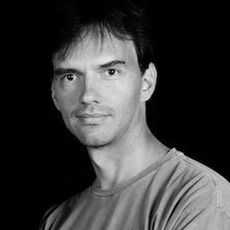
\includegraphics[width=2.6cm,height=2.6cm]{Images/Introduction/ErnestoBaschny.jpg}
			\end{figure}
		\end{column}

	\end{columns}

\end{frame}

% ------------------------------------------------------------------------------
% Standard Slide
% ------------------------------------------------------------------------------

\begin{frame}[fragile]
	% \TabPositions{1.2cm}

	\frametitle{Uvod}
	\framesubtitle{TYPO3 CMS 6.2 LTS: Cinjenice}

	\begin{itemize}
		\item Datum izlaska: 25. Mart 2014.
		\item Vreme razvoja i izlaska:
	\end{itemize}

	\begin{figure}
		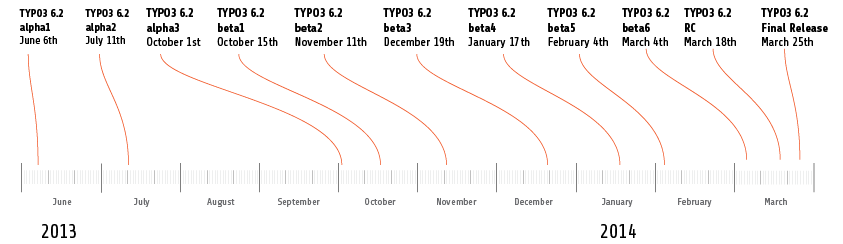
\includegraphics[width=0.99\linewidth]{Images/Introduction/ReleaseTimeline.png}
	\end{figure}

\end{frame}

% ------------------------------------------------------------------------------
% Standard Slide
% ------------------------------------------------------------------------------

\begin{frame}[fragile]
	\frametitle{Uvod}
	\framesubtitle{TYPO3 CMS 6.2 LTS: Cinjenice}

	\begin{itemize}
		\item Sistemski zahtevi
		\begin{itemize}
			\item PHP	\tabto{1.2cm} v5.3.7 - v5.5.x
			\item MySQL	\tabto{1.2cm} v5.1.x - v5.6.x
		\end{itemize}
	\end{itemize}

	\begin{itemize}
		\item Prestanak odrzavanja: 30 Decembar 2016
		\item TYPO3 CMS 6.2 je verzija sa \textbf{dugorocnom podrskom} (LTS) (podrska od 3 godine!)
	\end{itemize}

\end{frame}

% ------------------------------------------------------------------------------
% Standard Slide
% ------------------------------------------------------------------------------

\begin{frame}[fragile]
	\frametitle{Uvod}
	\framesubtitle{TYPO3 CMS 6.2 LTS: Cinjenice}

	\begin{itemize}
		\item Agenda izlaska:
	\end{itemize}

	\begin{figure}
		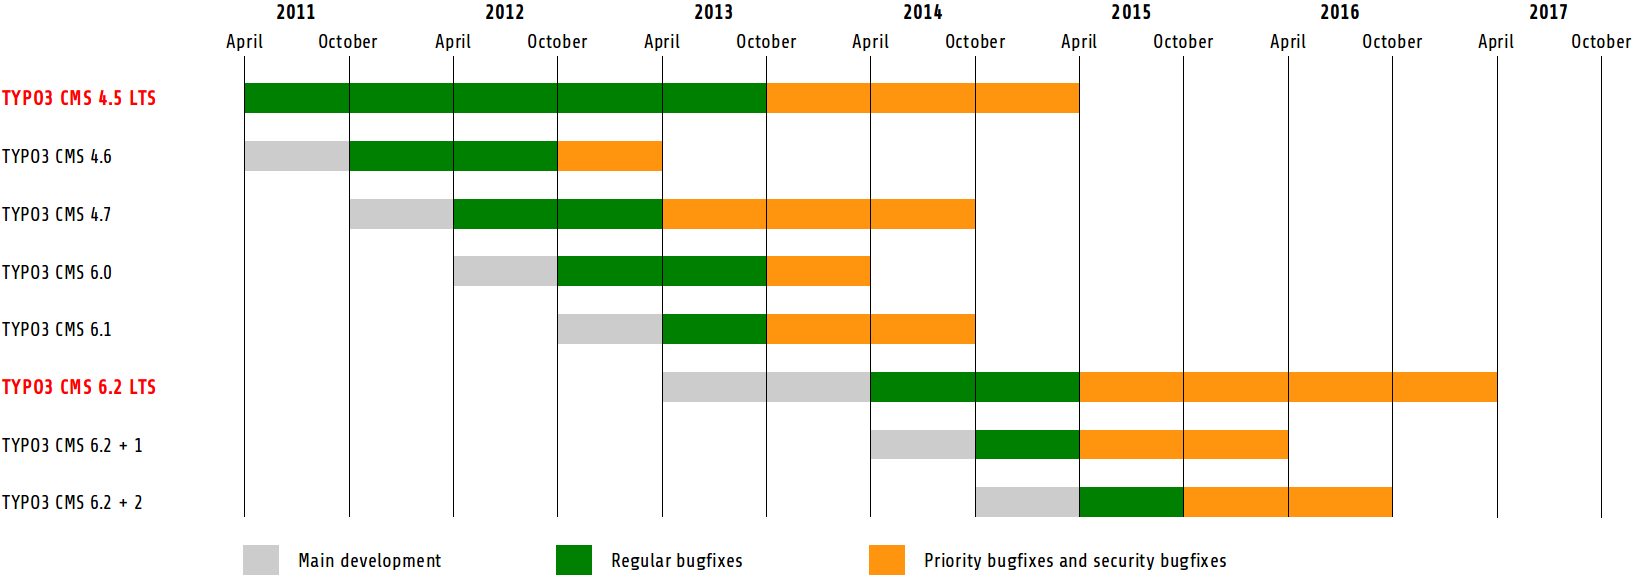
\includegraphics[width=0.99\linewidth]{Images/Introduction/ReleaseAgenda.png}
	\end{figure}

\end{frame}

% ------------------------------------------------------------------------------



% ------------------------------------------------------------------------------
% Chapter 1: Install Tool
% ------------------------------------------------------------------------------

% ------------------------------------------------------------------------------
% TYPO3 CMS 6.2 LTS - What's New - Chapter "Install Tool" (Spanish Version)
%
% @author	Sergio Catalá <sergio.catala@e-net.info>
% @author	Michel Mix <mmix@autistici.org>
% @license	Creative Commons BY-NC-SA 3.0
% @link		http://typo3.org/download/release-notes/whats-new/
% @language	Spanish
% ------------------------------------------------------------------------------
% Chapter: Install Tool
% ------------------------------------------------------------------------------

\section{Herramienta de Instalación}
\begin{frame}[fragile]
	\frametitle{Herramienta de Instalación}

	\begin{center}\huge{Capítulo 1:}\end{center}
	\begin{center}\huge{\color{typo3darkgrey}\textbf{La Herramienta de Instalación}}\end{center}

\end{frame}

% ------------------------------------------------------------------------------
% Installation
% ------------------------------------------------------------------------------

\begin{frame}[fragile]
	\frametitle{Herramienta de Instalación}
	\framesubtitle{Instalación (1)}

	\begin{itemize}
		\item Sólo se requiere \underline{un} paquete para una instalación:\newline
				\texttt{typo3\_src-6.2.x.tar.gz} (tamaño del fichero: aprox. 20MB)
		\item Los paquetes "Dummy" y "Blank" quedaron obsoletos
		\item Instalación:
			\begin{itemize}
				\item El paquete fuente se extrae en el directorio web raíz
				\item Se crean los enlaces simbólicos requeridos
				\item Apunte el navegador web a su directorio raíz
				\item El Instalador de TYPO3 empieza el asistente de 1-2-3-4-pasos
			\end{itemize}

	\end{itemize}

\end{frame}

% ------------------------------------------------------------------------------
% Installation
% ------------------------------------------------------------------------------

\begin{frame}[fragile]
	% \TabPositions{2cm}

	\frametitle{Herramienta de Instalación}
	\framesubtitle{Instalación (2)}

	\begin{itemize}
		\item El instalador se asegura de que todos los ficheros y directorios necesarios estén en su sitio
		\item Se crearán automáticamente los ficheros necesarios para una configuración personalizada
		\item Los siguientes enlaces simbólicos \underline{deben} existir:

		\begin{itemize}
			\item \texttt{typo3\_src}	\tabto{2cm} (apunta al directorio raíz de TYPO3)
			\item \texttt{typo3}		\tabto{2cm} (apunta al directorio: \texttt{typo3\_src/typo3})
			\item \texttt{index.php}	\tabto{2cm} (apunta al fichero: \texttt{typo3\_src/index.php})
		\end{itemize}

		\item ¡No se requieren más ficheros/directorios para instalar TYPO3!
		\item Directorio \texttt{t3lib} eliminado
		\item Más detalles: Guía de Instalación y Actualización de TYPO3\newline
			\url{http://docs.typo3.org/typo3cms/InstallationGuide}

	\end{itemize}

\end{frame}

% ------------------------------------------------------------------------------
% Re-Development
% ------------------------------------------------------------------------------

\begin{frame}[fragile]
	\frametitle{Herramienta de Instalación}
	\framesubtitle{Redesarrollo (1)}

	\begin{columns}[T]

		\begin{column}{.5\textwidth}
			\begin{itemize}
				\item Redesarrollado desde cero usando Fluid
				\item El \underline{primer} paso chequea el entorno del sistema y reporta asuntos
				\item Los asuntos reportados pueden arreglarse\newline (y re-testearse) o ignorarse
			\end{itemize}
		\end{column}

		\begin{column}{.5\textwidth}
			\begin{figure}\vspace*{-0.4cm}
				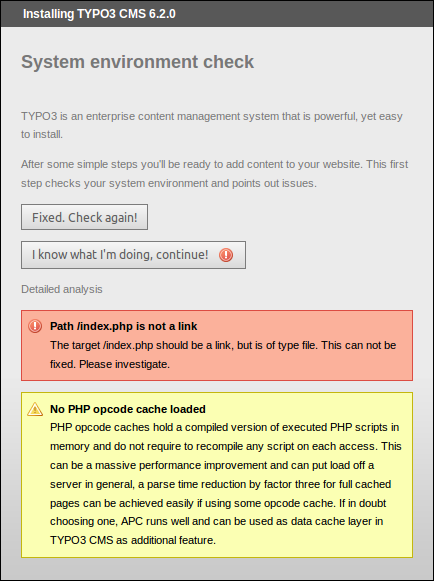
\includegraphics[width=0.8\linewidth]{Images/InstallTool/SystemEnvironmentCheck.png}
			\end{figure}
		\end{column}

	\end{columns}

\end{frame}

% ------------------------------------------------------------------------------
% Re-Development
% ------------------------------------------------------------------------------

\begin{frame}[fragile]
	\frametitle{Herramienta de Instalación}
	\framesubtitle{Redesarrollo (2)}

	\begin{columns}[T]

		\begin{column}{.5\textwidth}
			\begin{itemize}
				\item La configuración inválida del núcleo (p.ej. no enlaces simbólicos como se recomienda) se reporta como un asunto, también
			\end{itemize}
		\end{column}

		\begin{column}{.5\textwidth}
			\begin{figure}\vspace*{-0.4cm}
				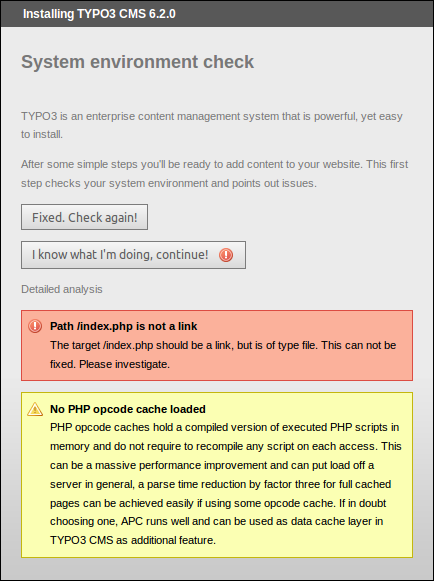
\includegraphics[width=0.8\linewidth]{Images/InstallTool/SystemEnvironmentCheck.png}
			\end{figure}
		\end{column}

	\end{columns}

\end{frame}

% ------------------------------------------------------------------------------
% Re-Development
% ------------------------------------------------------------------------------

\begin{frame}[fragile]
	\frametitle{Herramienta de Instalación}
	\framesubtitle{Redesarrollo (3)}

	\begin{columns}[T]

		\begin{column}{.5\textwidth}
			\begin{itemize}
				\item El \underline{segundo} paso permite a los usuarios introducir los detalles de acceso a la base de datos
				\item Se pueden seleccionar tipos de conexión
					\begin{itemize}
						\item Conexión basada en TCP/IP
						\item Conexión basada en Socket
					\end{itemize}
				\item Son también posibles alternativas a MySQL
			\end{itemize}
		\end{column}

		\begin{column}{.5\textwidth}
			\begin{figure}\vspace*{-0.4cm}
				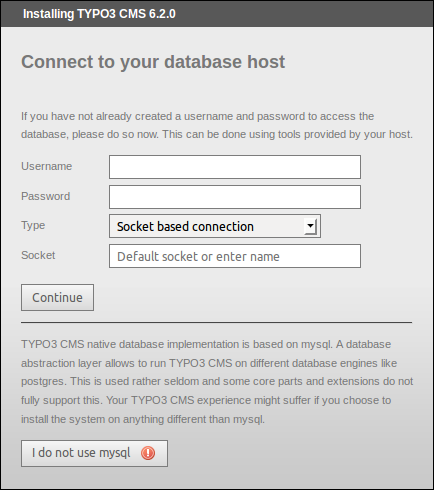
\includegraphics[width=0.8\linewidth]{Images/InstallTool/DatabaseConnectionDetails.png}
			\end{figure}
		\end{column}

	\end{columns}

\end{frame}

% ------------------------------------------------------------------------------
% Re-Development
% ------------------------------------------------------------------------------

\begin{frame}[fragile]
	\frametitle{Herramienta de Instalación}
	\framesubtitle{Redesarrollo (4)}

	\begin{columns}[T]

		\begin{column}{.5\textwidth}
			\begin{itemize}
				\item El \underline{tercer} paso permite a los usuarios seleccionar/crear la base de datos\newline
					(como en TYPO3 < 6.2)
				\item El \underline{cuarto} paso permite a los usuarios fijar una contraseña para el usuario "admin"\newline (que es también la contraseña inicial de la Herramienta de Instalación) y un nombre para el sitio
			\end{itemize}
		\end{column}

		\begin{column}{.5\textwidth}
			\begin{figure}\vspace*{-0.4cm}
				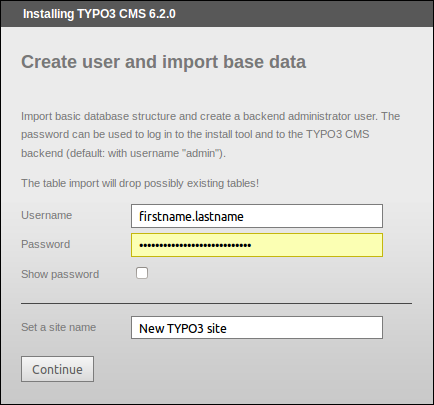
\includegraphics[width=0.8\linewidth]{Images/InstallTool/AdminPasswordAndSiteName.png}
			\end{figure}
		\end{column}

	\end{columns}

\end{frame}

% ------------------------------------------------------------------------------
% Delete All Cache
% ------------------------------------------------------------------------------

\begin{frame}[fragile]
	\frametitle{Herramienta de Instalación}
	\framesubtitle{Borrar Toda la Caché (1)}

	\begin{itemize}
		\item Nueva función bajo "Acciones importantes" permite a los usuarios borrar toda la caché
		\item Esto también funciona, si la caché contiene código PHP inválido\newline
			(lo que posiblemente bloquee TYPO3 CMS)
		\item Se puede evitar una instancia TYPO3 que no funciona accediendo a la Herramienta de Instalación directamente: \texttt{http://example.com/typo3/install}
	\end{itemize}

	\begin{columns}[T]
		\begin{column}{.3\textwidth}
			\begin{figure}\vspace*{-0.4cm}
				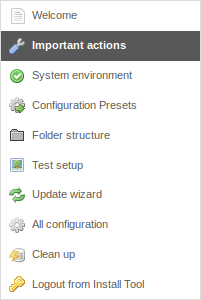
\includegraphics[width=0.7\linewidth,height=3cm]{Images/InstallTool/ImportantActions.png}
			\end{figure}
		\end{column}
		\begin{column}{.7\textwidth}
			\begin{figure}\vspace*{-0.4cm}
				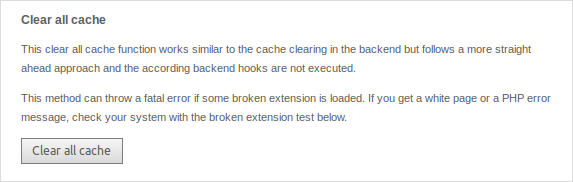
\includegraphics[width=0.9\linewidth]{Images/InstallTool/ClearAllCache.png}
			\end{figure}
		\end{column}
	\end{columns}

\end{frame}

% ------------------------------------------------------------------------------
% Delete All Cache
% ------------------------------------------------------------------------------

\begin{frame}[fragile]
	\frametitle{Herramienta de Instalación}
	\framesubtitle{Borrar Toda la Caché (2)}

	Secuencia de acciones al ejecutar "Borrar toda la caché":

	\begin{enumerate}
		\item Se borra el contenido del directorio \texttt{typo3temp/Cache}
		\item Se vacían las tablas \texttt{cf\_*} de la base de datos
		\item Se cargan los ficheros \texttt{ext\_localconf.php} y \texttt{ext\_tables.php}\newline
			de las extensiones
		\item Se ejecuta \texttt{flushCaches()}
	\end{enumerate}

\end{frame}

% ------------------------------------------------------------------------------
% Check For Broken Extensions
% ------------------------------------------------------------------------------

\begin{frame}[fragile]
	\frametitle{Herramienta de Instalación}
	\framesubtitle{Chequeo de Extensiones Rotas}

	\begin{itemize}
		\item Nueva función bajo "Acciones importantes" deja a los usuarios chequear, si se pueden cargar extensiones sin romper el sistema
		\item Muy útil para una actualización de TYPO3 4.5 a 6.2
	\end{itemize}

	\begin{columns}[T]
		\begin{column}{.3\textwidth}
			\begin{figure}\vspace*{-0.4cm}
				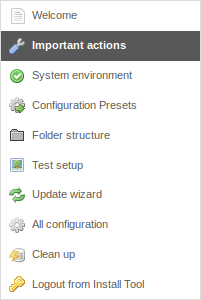
\includegraphics[width=0.7\linewidth]{Images/InstallTool/ImportantActions.png}
			\end{figure}
		\end{column}
		\begin{column}{.7\textwidth}
			\begin{figure}\vspace*{-0.4cm}
				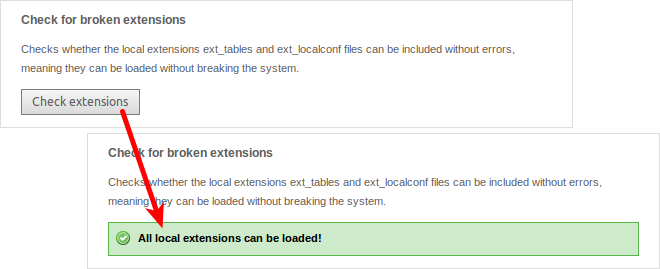
\includegraphics[width=1\linewidth]{Images/InstallTool/CheckForBrokenExtensions.png}
			\end{figure}
		\end{column}
	\end{columns}

\end{frame}

% ------------------------------------------------------------------------------
% Increased Security: Salted Passwords
% ------------------------------------------------------------------------------

\begin{frame}[fragile]
	\frametitle{Herramienta de Instalación}
	\framesubtitle{Contraseñas Salted}

	\begin{itemize}
		\item Al crear el nuevo usuario administrador del backend vía la Herramienta de Instalación, se usa una contraseña \textbf{salted}\newline
			\smaller(requiere que esté instalada, cargada y configurada EXT:saltedpasswords)\normalsize
		\item La contraseña de la Herramienta de Instalación es una contraseña \textbf{salted} también
			\smaller(los MD5 hashes existentes se convierten automáticamente en el primer inicio de sesión)\normalsize
	\end{itemize}

	\begin{columns}[T]
		\begin{column}{.3\textwidth}
			\begin{figure}\vspace*{-0.4cm}
				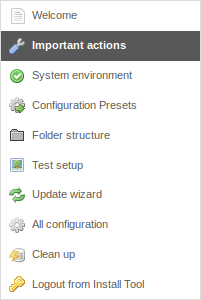
\includegraphics[width=0.7\linewidth]{Images/InstallTool/ImportantActions.png}
			\end{figure}
		\end{column}
		\begin{column}{.7\textwidth}
			\begin{figure}\vspace*{-0.4cm}
				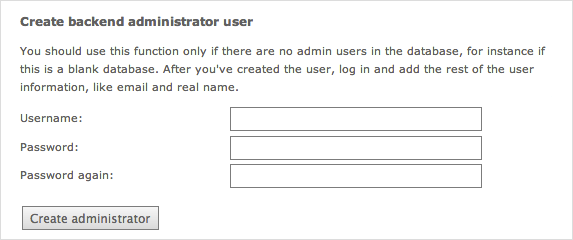
\includegraphics[width=0.9\linewidth]{Images/InstallTool/SaltedPasswords.png}
			\end{figure}
		\end{column}
	\end{columns}

\end{frame}

% ------------------------------------------------------------------------------
% Application Context
% ------------------------------------------------------------------------------

\begin{frame}[fragile]
	\frametitle{Herramienta de Instalación}
	\framesubtitle{Contexto de la Aplicación}

	\begin{itemize}
		\item TYPO3 >= 6.2 tiene en cuenta el \textbf{Contexto de la Aplicación}\newline
			\smaller(conocido en TYPO3 Flow)\normalsize
		\item La variable de entorno \texttt{TYPO3\_CONTEXT} fija el contexto\newline
			\smaller(por defecto: \texttt{Production}, subcontexto tal como \texttt{Production/Staging} posible)\normalsize

			\begin{lstlisting}
				# Fichero: .htaccess
				# Reglas para fijar el Contexto basada en el nombre del host:

				RewriteCond %{HTTP_HOST} ^dev\.example\.com$
				RewriteRule (.*) $1 [E=TYPO3_CONTEXT:Development]

				RewriteCond %{HTTP_HOST} ^www\.example\.com$
				RewriteRule (.*) $1 [E=TYPO3_CONTEXT:Production]

				# Fija una variable de entorno, disponible ahora en TYPO3 CMS:
				SetEnv TYPO3_CONTEXT Production
			\end{lstlisting}

	\end{itemize}

\end{frame}

% ------------------------------------------------------------------------------
% Application Context
% ------------------------------------------------------------------------------

\begin{frame}[fragile]
	\frametitle{Herramienta de Instalación}
	\framesubtitle{Presets de Ajustes en TYPO3\_CONF\_VAR (1)}

	\begin{columns}[T]
		\begin{column}{.5\textwidth}

			\begin{itemize}
				\item Ciertos ajustes \texttt{TYPO3\_CONF\_VAR} pueden configurarse en la Herramienta de Instalación
				\item Ajustes como la salida de depuración, el registro de discontinuación, devIPmask y otros registros del sistema y niveles de registro
			\end{itemize}

		\end{column}
		\begin{column}{.5\textwidth}

			\begin{figure}\vspace*{-0.4cm}
				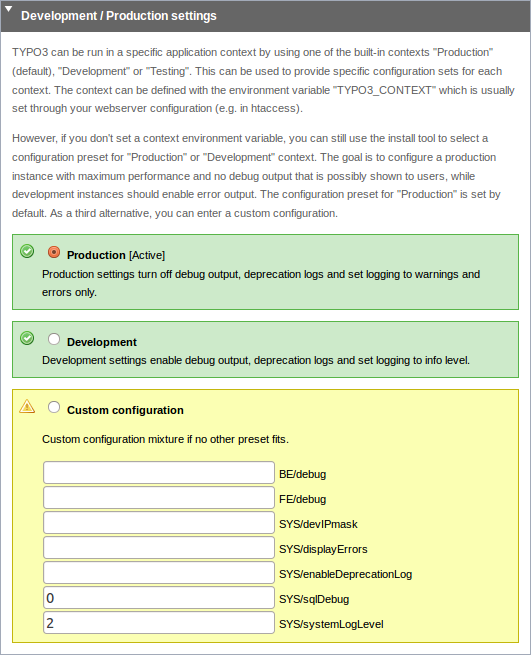
\includegraphics[width=0.8\linewidth]{Images/InstallTool/ApplicationContext.png}
			\end{figure}

		\end{column}
	\end{columns}

\end{frame}

% ------------------------------------------------------------------------------
% Application Context
% ------------------------------------------------------------------------------

\begin{frame}[fragile]
	\frametitle{Herramienta de Instalación}
	\framesubtitle{Presets de Ajustes en TYPO3\_CONF\_VAR (2)}

	\begin{columns}[T]
		\begin{column}{.5\textwidth}

			\begin{itemize}
				\item Contextos incorporados: "Production" y "Development"\newline
					(es posible una configuración personalizada)
			\end{itemize}

		\end{column}
		\begin{column}{.5\textwidth}

			\begin{figure}\vspace*{-0.4cm}
				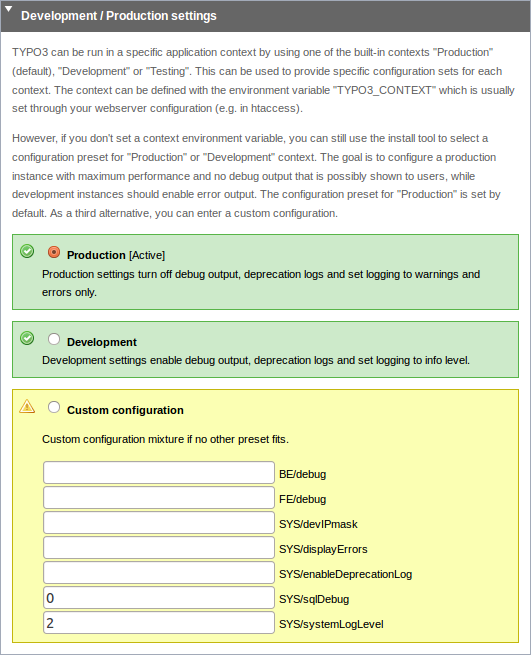
\includegraphics[width=0.8\linewidth]{Images/InstallTool/ApplicationContext.png}
			\end{figure}

		\end{column}
	\end{columns}

\end{frame}

% ------------------------------------------------------------------------------
% Improved Usability
% ------------------------------------------------------------------------------

\begin{frame}[fragile]
	\frametitle{Herramienta de Instalación}
	\framesubtitle{Usabilidad Mejorada}

	\begin{columns}[T]
		\begin{column}{.5\textwidth}

			\begin{itemize}
				\item Posición fija del menú de la izquierda al hacer scroll
					\begingroup\color{typo3red}\textbf{(1)}\endgroup
				\item Posición fija del botón "Escribir configuración" en la parte inferior
					\begingroup\color{typo3red}\textbf{(2)}\endgroup
				\item Se agrupan y ordenan las entradas de "Toda la Configuración" (se despliega una sección haciendo clic en el encabezamiento)
					\begingroup\color{typo3red}\textbf{(3)}\endgroup
			\end{itemize}

		\end{column}
		\begin{column}{.5\textwidth}

			\begin{figure}\vspace*{-0.4cm}
				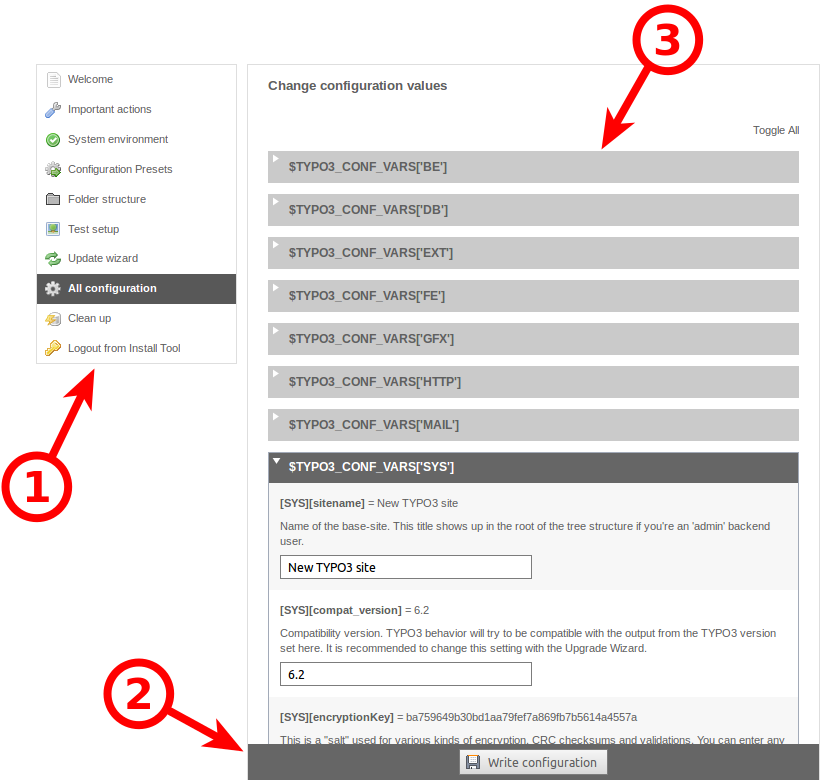
\includegraphics[width=0.8\linewidth]{Images/InstallTool/ImprovedUsability.png}
			\end{figure}

		\end{column}
	\end{columns}

\end{frame}

% ------------------------------------------------------------------------------
% Human-Friendly Error Codes
% ------------------------------------------------------------------------------

\begin{frame}[fragile]
	\frametitle{Herramienta de Instalación}
	\framesubtitle{Códigos de Error Amistosos}

	\begin{itemize}
		\item Pueden usarse palabras clave significativas para las siguientes opciones:\newline
			(TYPO3 < 6.2: sólo valores numéricos)
	\end{itemize}

	\begin{columns}[T]
		\begin{column}{.4\textwidth}
			\advance\leftskip+0.8cm

			\smaller
				\texttt{[SYS][errorHandlerErrors]}\newline
				\texttt{[SYS][exceptionalErrors]}\newline
				\texttt{[SYS][syslogErrorReporting]}\newline
				\texttt{[SYS][belogErrorReporting]}\newline
			\normalsize

		\end{column}
		\begin{column}{.6\textwidth}

			\begin{figure}\vspace*{-0.4cm}
				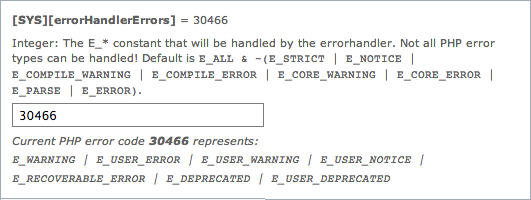
\includegraphics[width=0.9\linewidth]{Images/InstallTool/HumanFriendlyErrorCodes.png}
			\end{figure}

		\end{column}
	\end{columns}

	\vspace{0.2cm}

	\begin{itemize}
		\item Un ViewHelper Extbase \textbf{format.phpErrorCode} se encarga de la conversión a códigos de error en PHP
	\end{itemize}

\end{frame}

% ------------------------------------------------------------------------------
% Errors In Folder Structure
% ------------------------------------------------------------------------------

\begin{frame}[fragile]
	\frametitle{Herramienta de Instalación}
	\framesubtitle{Errores en Estructura de Carpeta}

	\begin{itemize}
		\item Se listan errores bajo "Estructura de Carpeta" con un símbolo (número rodeado por un círculo)
	\end{itemize}

	\begin{figure}
		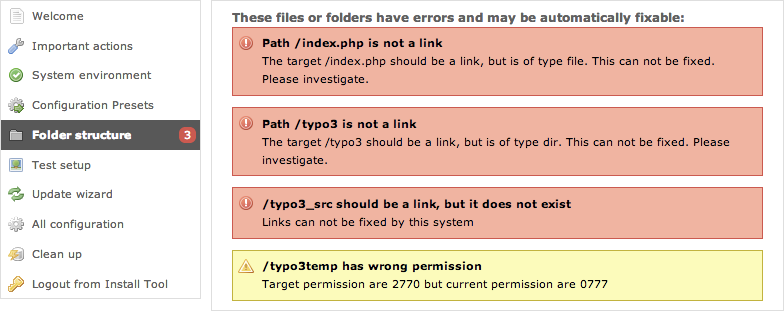
\includegraphics[width=0.95\linewidth]{Images/InstallTool/ErrorsInFolderStructure.png}
	\end{figure}

\end{frame}

% ------------------------------------------------------------------------------
% Core Updates
% ------------------------------------------------------------------------------

\begin{frame}[fragile]
	\frametitle{Herramienta de Instalación}
	\framesubtitle{Actualizaciones del Núcleo}

	\begin{itemize}
		\item El núcleo de TYPO3 se actualiza a su última versión menor con un click de botón
		\item La variable de entorno \texttt{TYPO3\_DISABLE\_CORE\_UPDATER=1} desactiva esta característica
	\end{itemize}

	\begin{figure}
		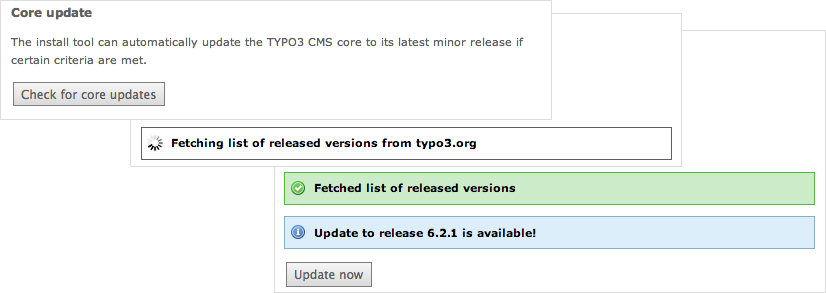
\includegraphics[width=0.95\linewidth]{Images/InstallTool/CoreUpdate.png}
	\end{figure}

\end{frame}

% ------------------------------------------------------------------------------
% Miscellaneous
% ------------------------------------------------------------------------------

\begin{frame}[fragile]
	\frametitle{Herramienta de Instalación}
	\framesubtitle{Varios (1)}

	\begin{itemize}
		\item Todos los formularios están protegidos con CSRF\newline
			  (\textit{cross-site request forgery})
		\item La Herramienta de Instalación usa una\newline
		 	  Vista Fluid Standalone simplificada
		\item Sólo se cargan las funciones TYPO3 esenciales\newline
			(\texttt{ext\_localconf.php} o \texttt{ext\_tables.php} corruptos de extensiones no pueden romper la Herramienta de Instalación nunca más)
		\item Nuevo punto de inicio:\newline
			\texttt{typo3/sysext/install/Start/Install.php}\newline
			Antes:					\tabto{3.2cm} \texttt{typo3/install/index.php}\newline
									\tabto{3.2cm} (existe una redirección desde la vieja URL a la nueva)
	\end{itemize}

\end{frame}

\begin{frame}[fragile]
	\frametitle{Herramienta de Instalación}
	\framesubtitle{Varios (2)}

	\begin{itemize}
		\item La caché desactivada asegura que la Herramienta de Instalación permanece usable, incluso si la caché contiene código PHP inválido
		\item Chequea si la opción de PHP \texttt{xdebug.max\_nesting\_level} muestra un valor de 250 o superior (el valor por defecto "100" probablemente causa problemas)
		\item "Chequeo de permisos relajado":

			\small
				Si la carpeta del directorio raíz no tiene los permisos correctos  (p.ej. "2770"),
				y no puede solucionarse esto, p.ej. porque el directorio no pertenece
				al usuario del sistema que corre la Herramienta de Instalación, el primer paso de la instalación
				se rompe.
				La opción "targetPermissionRelaxed" reduce la severidad si los permisos no son
				ideales y permite continuar con la instalación mientras puedan crearse las subcarpetas necesarias.
			\normalsize
	\end{itemize}

\end{frame}

% ------------------------------------------------------------------------------
% Miscellaneous
% ------------------------------------------------------------------------------

\begin{frame}[fragile]
	\frametitle{Herramienta de Instalación}
	\framesubtitle{Varios (3)}

	\begin{itemize}
		\item Borradas las opciones (claves) de la Herramienta de Instalación\newline
			\small(y por tanto del fichero \texttt{LocalConfiguration.php}, también):\normalsize
	\end{itemize}

	\begin{columns}[T]
		\begin{column}{.5\textwidth}
			\advance\leftskip+0.8cm
			\smaller
				\texttt{BE/loginLabels}\newline
				\texttt{BE/loginNews}\newline
				\texttt{BE/useOnContextMenuHandler}\newline
				\texttt{EXT/em\_mirrorListURL}\newline
				\texttt{EXT/em\_wsdlURL}\newline
				\texttt{EXT/extList}\newline
				\texttt{EXT/extList\_FE}\newline
				\texttt{EXT/noEdit}\newline
			\normalsize
		\end{column}
		\begin{column}{.5\textwidth}
			\smaller
				\texttt{FE/defaultTypoScript\_editorcfg}\newline
				\texttt{FE/simulateStaticDocuments}\newline
				\texttt{GFX/noIconProc}\newline
				\texttt{GFX/TTFLocaleConv}\newline
				\texttt{SYS/additionalAllowedClassPrefixes}\newline
				\texttt{SYS/caching/cacheBackends}\newline
				\texttt{SYS/caching/cacheFrontends}\newline
				\texttt{SYS/extCache}\newline
				\texttt{SYS/T3instID}\newline
			\normalsize
		\end{column}

	\end{columns}

\end{frame}

% ------------------------------------------------------------------------------



% ------------------------------------------------------------------------------
% Chapter 2: TYPO3 CMS Goes Responsive
% ------------------------------------------------------------------------------

% ------------------------------------------------------------------------------
% TYPO3 CMS 6.2 LTS - What's New - Chapter "Responsive Images" (Italian Version)
%
% @author Roberto Torresani <roberto.torresani@typo3.org>
% @license	Creative Commons BY-NC-SA 3.0
% @link		http://typo3.org/download/release-notes/whats-new/
% @language	Italian
% ------------------------------------------------------------------------------
% Chapter: Responsive Images
% ------------------------------------------------------------------------------

\section{Immagini responsive}
\begin{frame}[fragile]
	\frametitle{Immagini responsive}

	\begin{center}\huge{Capitolo 2:}\end{center}
	\begin{center}\huge{\color{typo3darkgrey}\textbf{Immagini responsive}}\end{center}

\end{frame}

% ------------------------------------------------------------------------------
% Select Screen Size In Page Preview
% ------------------------------------------------------------------------------

\begin{frame}[fragile]
	\frametitle{Immagini responsive}
	\framesubtitle{Seleziona le dimensioni dello schermo nell'anteprima di pagina}

	\begin{itemize}
		\item Gli editor possono selezionare le dimensioni dello schermo nel modulo "View" per verificare i siti responsivi
	\end{itemize}

	\begin{figure}
		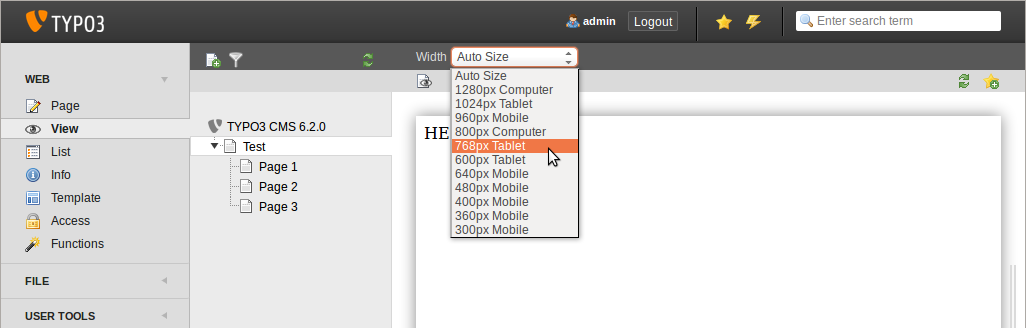
\includegraphics[width=0.95\linewidth]{Images/ResponsiveImages/ScreenSizeInPagePreview.png}
	\end{figure}

\end{frame}

% ------------------------------------------------------------------------------
% Customize Available Screen Sizes
% ------------------------------------------------------------------------------

\begin{frame}[fragile]
	\frametitle{Immagini responsive}
	\framesubtitle{Personalizzazione delle dimensioni di schermo}

	\begin{itemize}
		\item Le dimensioni dello schermo sono configurabili in PageTSconfig:

		\lstset{
			basicstyle=\fontsize{7}{9}\selectfont\ttfamily
		}

		\begin{lstlisting}
			mod.web_view.previewFrameWidths {
			  1780.label = <any LLL or string>
			  1780.height = 145
			}
		\end{lstlisting}

		\item La larghezza è definita dalla chiave (nell'esempio: 1780), l'altezza è un opzione
		\item Le dimensioni predefinite possono essere trovate nel file:\newline
			\small\texttt{typo3/sysext/core/Configuration/DefaultConfiguration.php}\normalsize
		\item Le etichette possono essere definite con PageTSconfig:

		\begin{lstlisting}
			mod.web_view.previewFrameWidths {
			  1280.label = LLL:EXT:viewpage/Resources/Private/Language/locallang.xlf:computer
			  1024.label = LLL:EXT:viewpage/Resources/Private/Language/locallang.xlf:tablet
			}
		\end{lstlisting}

	\end{itemize}

\end{frame}

% ------------------------------------------------------------------------------
% Responsive Image Galleries
% ------------------------------------------------------------------------------

\begin{frame}[fragile]
	\frametitle{Immagini responsive}
	\framesubtitle{Galleria delle immagini responsive}

	\begin{itemize}
		\item Attributi aggiuntivi per utilizzare gallerie di immagini responsive
		\item sono state aggiunte in "CSS styled content"
		\item Esempio: HTML5 (richiede \texttt{config.doctype = html5})\newline

			TYPO3 CMS < 6.2:

			\lstset{
				basicstyle=\fontsize{7}{9}\selectfont\ttfamily
			}

			\begin{lstlisting}
				<div class="csc-textpic-imagewrap">...</div>
			\end{lstlisting}

			TYPO3 CMS >= 6.2:

			\begin{lstlisting}
				<div class="csc-textpic-imagewrap"
				  data-csc-images="{register:imageCount}"
				  data-csc-cols="{field:imagecols}">...</div>
			\end{lstlisting}

	\end{itemize}

\end{frame}

% ------------------------------------------------------------------------------
% Responsive Image Rendering
% ------------------------------------------------------------------------------

\begin{frame}[fragile]
	\frametitle{Immagini responsive}
	\framesubtitle{Visualizzazione di immagine responsiva}

	\begin{itemize}
		\item La visualizzazione del cObject IMAGE usa una "sourceCollection" per supportare le varie dimensioni di schermo
		\item nel visualizzare immagini responsive per i cObjects "testo/immagine" e "immagini" richiedendo due configurazioni nel Constant Editor:

			\texttt{styles.content.imgtext.responsive}\newline
			\texttt{styles.content.imgtext.layoutKey}

		\item Le opzioni valide sono:

			\begin{itemize}
				\item \texttt{default}:	\tabto{2cm} default tag \texttt{<img>}
				\item \texttt{srcset}:	\tabto{2cm} \texttt{<img>}-tag con sorgente alternativa come attributo srcset
				\item \texttt{picture}:	\tabto{2cm} \texttt{<picture>}-tag con tag sorgente figlio
				\item \texttt{data}:	\tabto{2cm} \texttt{<img>}-tag con sorgente alternativa come attributo data
			\end{itemize}

	\end{itemize}

\end{frame}

% ------------------------------------------------------------------------------
% Property: layoutKey
% ------------------------------------------------------------------------------

\begin{frame}[fragile]
	\frametitle{Immagini responsive}
	\framesubtitle{Proprietà: layoutKey}

	\begin{itemize}
		\item \texttt{layoutKey} definisce il layout di visualizzazione\newline
			(è il codice HTML, utilizzato per il tag \texttt{<img>})
		\item Ogni opzione mostra un comportamento univoco per la visualizzazione dell'HTML
		\item L'opzione \texttt{default} visualizza il tag \texttt{<img>} tradizionalmente\newline
			(viene utilizzato se il sito non è responsivo)
		\item L'implementazione di un sito responsivo necessita di immagini con dimensioni differenti nelle varie risoluzioni e grandezza di schermo
		\item Dipende dal framework HTML, browser e libreria JavaScript (per il miglioramento progressivo):

			\begin{itemize}
				\item usa uno dei layout predefiniti o
				\item definisci un tuo layout personalizzato
			\end{itemize}

	\end{itemize}

\end{frame}

% ------------------------------------------------------------------------------
% Property: layout
% ------------------------------------------------------------------------------

\begin{frame}[fragile]
	\frametitle{Immagini responsive}
	\framesubtitle{Proprietà: layout}

			\lstset{
				basicstyle=\tiny\ttfamily
			}

			\begin{lstlisting}
				layoutKey = {$styles.content.imgtext.layoutKey}
				layout {
				  default {
				    element = <img src="###SRC###" width="###WIDTH###" height="###HEIGHT###" ###PARAMS###
				      ###ALTPARAMS### ###BORDER######SELFCLOSINGTAGSLASH###>
				  }
				  srcset {
				    element = <img src="###SRC###" srcset="###SOURCECOLLECTION###" ###PARAMS###
				      ###ALTPARAMS### ###SELFCLOSINGTAGSLASH###>
				    source = |*|###SRC### ###SRCSETCANDIDATE###,|*|###SRC### ###SRCSETCANDIDATE###
				  }
				  picture {
				    element = <picture>###SOURCECOLLECTION###<img src="###SRC###" ###PARAMS###
				      ###ALTPARAMS######SELFCLOSINGTAGSLASH###></picture>
				    source = <source src="###SRC###" media="###MEDIAQUERY###"###SELFCLOSINGTAGSLASH###>
				  }
				  data {
				    element = <img src="###SRC###" ###SOURCECOLLECTION### ###PARAMS###
				      ###ALTPARAMS######SELFCLOSINGTAGSLASH###>
				    source = data-###DATAKEY###="###SRC###"
				  }
				}
			\end{lstlisting}

\end{frame}

% ------------------------------------------------------------------------------
% Property: layout.[layoutKey].element
% ------------------------------------------------------------------------------

\begin{frame}[fragile]
	\frametitle{Immagini responsive}
	\framesubtitle{Proprietà: layout.[layoutKey].element}


	\begin{itemize}
			\item \lstinline!###SRC###!\newline
				URL per l'attributo: \texttt{src}

			\item \lstinline!###WIDTH###!\newline
				Larghezza dell'immagine (in pixel) per l'attributo: \texttt{width}

			\item \lstinline!###HEIGHT###!\newline
				Altezza dell'immagine (in pixel) per l'attributo: \texttt{height}

			\item \lstinline!###PARAMS###!\newline
				Parametri aggiuntivi come definiti nel cObject IMAGE

			\item \lstinline!###ALTPARAMS###!\newline
				Parametri alternativi aggiuntivi come definiti nel cObject IMAGE

	\end{itemize}

\end{frame}

% ------------------------------------------------------------------------------
% Property: layout.[layoutKey].element
% ------------------------------------------------------------------------------

\begin{frame}[fragile]
	\frametitle{Immagini responsive}
	\framesubtitle{Proprietà: layout.[layoutKey].element}

		\begin{itemize}
			\item \lstinline!###BORDER###!\newline
				Bordo (in pixel) per l'attributo: \texttt{border}

			\item \lstinline!###SELFCLOSINGTAGSLASH###!\newline
				Tag di chiusura, es. \texttt{<img ... />} invece di \texttt{<img ... >}\newline
				(dipende da \texttt{config.xhtmlDoctype} o \texttt{config.doctype})

			\item \lstinline!###SOURCECOLLECTION###!\newline
				Sorgente aggiuntiva dell'immagine, dipende dall'uso responsivo nel design.
				L'esatto valore è definito nella chiave: \texttt{layout.[layoutKey].source}

	\end{itemize}

\end{frame}

% ------------------------------------------------------------------------------
% Property: sourceCollection.[dataKey]
% ------------------------------------------------------------------------------

\begin{frame}[fragile]
	\frametitle{Immagini responsive}
	\framesubtitle{Proprietà: sourceCollection.[dataKey]}

	\begin{itemize}
		\item sourceCollection di default di EXT:css\_styled\_content
		\item è fortemente suggerito scrivere la propria sourceCollection

			\lstset{
				basicstyle=\tiny\ttfamily
			}

			\begin{lstlisting}
				sourceCollection {
				  small {
				    width = 200
				    srcsetCandidate = 600w
				    mediaQuery = (max-device-width: 600px)
				    dataKey = small
				  }
				  smallRetina {
				    if.directReturn = 1
				    width = 200
				    pixelDensity = 2
				    srcsetCandidate = 600w 2x
				    mediaQuery = (max-device-width: 600px) AND (min-resolution: 192dpi)
				    dataKey = smallRetina
				  }
				}
			\end{lstlisting}
	\end{itemize}

\end{frame}

% ------------------------------------------------------------------------------
% Further Resources (External Links)
% ------------------------------------------------------------------------------

\begin{frame}[fragile]
	\frametitle{Immagini responsive}
	\framesubtitle{Ulteriori risorse}

	\begin{itemize}
		\item Esempi di codice funzionante:\newline
			\small\url{http://wiki.typo3.org/Responsive_Image_Rendering}\normalsize

		\item Articolo di Sven Wolfermann su typo3.org:\newline
			\small\url{http://typo3.org/news/article/responsive-image-rendering-in-typo3-cms-62/}\normalsize

		\item W3C specification:\newline
			\small\url{http://www.w3.org/html/wg/drafts/srcset/w3c-srcset/}\newline
			\small\url{http://www.w3.org/TR/html-picture-element/}

		\item Lavori e progetti del "Responsive Image Community Group":\newline
			\small\url{http://responsiveimages.org}\normalsize

	\end{itemize}

\end{frame}

% ------------------------------------------------------------------------------



% ------------------------------------------------------------------------------
% Chapter 3: Backend Changes
% ------------------------------------------------------------------------------

% ------------------------------------------------------------------------------
% TYPO3 CMS 6.2 LTS - What's New - Chapter "Backend Changes" (Russian Version)
%
% @author	Andrey Aksenov <aksenovaa@bk.ru>
% @license	Creative Commons BY-NC-SA 3.0
% @link		http://typo3.org/download/release-notes/whats-new/
% @language	Russian
% ------------------------------------------------------------------------------
% Chapter: Backend Changes
% ------------------------------------------------------------------------------

\section{Изменение во внутреннем интерфейсе}
\begin{frame}[fragile]
	\frametitle{Изменение во внутреннем интерфейсе}

	\begin{center}\huge{Глава 3:}\end{center}
	\begin{center}\huge{\color{typo3darkgrey}\textbf{Изменение во внутреннем интерфейсе}}\end{center}

\end{frame}

% ------------------------------------------------------------------------------
% Autofocus
% ------------------------------------------------------------------------------
% http://forge.typo3.org/issues/49228

\begin{frame}[fragile]
	\frametitle{Изменение во внутреннем интерфейсе}
	\framesubtitle{Авторизация}

 	\begin{itemize}
		\item Автоматически в фокусе оказывается поле "имя пользователя" (username)\newline
			(HTML5 атрибут: \texttt{autofocus="autofocus"})
	\end{itemize}

	\begin{figure}
		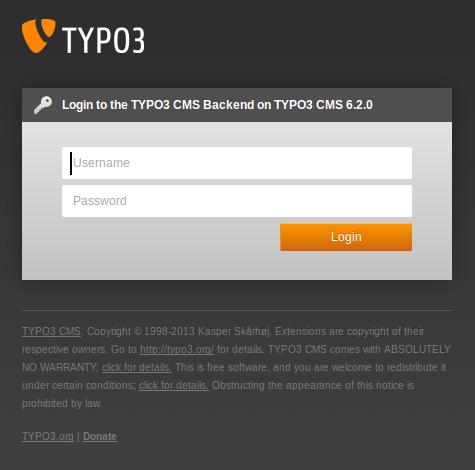
\includegraphics[width=0.4\linewidth]{Images/BackendChanges/BackendLogin.png}
	\end{figure}

\end{frame}

% ------------------------------------------------------------------------------
% Visual Appearance
% ------------------------------------------------------------------------------
% http://forge.typo3.org/issues/48376

\begin{frame}[fragile]
	\frametitle{Изменение во внутреннем интерфейсе}
	\framesubtitle{Внешний вид}

	\begin{columns}[T]

		\begin{column}{.5\textwidth}
			\begin{itemize}
				\item Макет стал удобнее и оживился
				\item Уменьшены отступы между элементами модуля (левый столбец)
				\item В основе лежит 12-колонная сетка, удвоенная
			\end{itemize}

			\advance\leftskip+3.8cm

            \smaller
                Слева: TYPO3 4.5\newline
                Справа: TYPO3 6.2
            \normalsize
		\end{column}

		\begin{column}{.5\textwidth}
			\begin{figure}\vspace*{-0.4cm}
				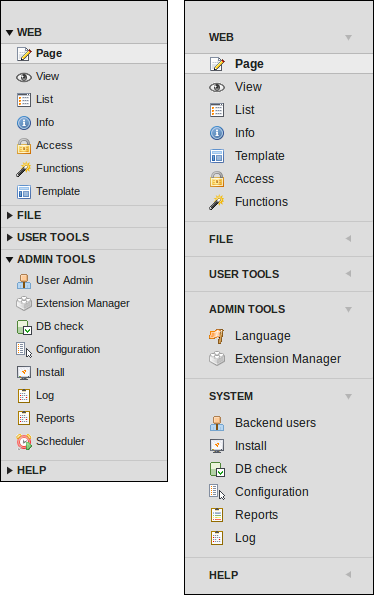
\includegraphics[width=0.6\linewidth]{Images/BackendChanges/VisualAppearance.png}
			\end{figure}
		\end{column}

	\end{columns}

\end{frame}

% ------------------------------------------------------------------------------
% Visual Appearance
% ------------------------------------------------------------------------------

\begin{frame}[fragile]
	\frametitle{Изменение во внутреннем интерфейсе}
	\framesubtitle{Внешний вид}

	\begin{columns}[T]

		\begin{column}{.5\textwidth}

			\begin{itemize}
				\item Изменена структура модулей в левом столбце
				\item Разделен на две части модуль "Инструменты управления" ("Admintools"):

					\begin{itemize}
						\item \textbf{Инструменты управления – Admintools} ("Языки"/"Languages" и "Расширения"/"Extension
						Manager")
						\item \textbf{Система – System} (низкоуровневые инструменты, без столбца дерева страниц)
					\end{itemize}

				\item Удален модуль "Справка TypoScript"/"TypoScript Help" (устарел)
				"TypoScript-Help"

			\end{itemize}

		\end{column}

		\begin{column}{.5\textwidth}
			\begin{figure}\vspace*{-0.4cm}
				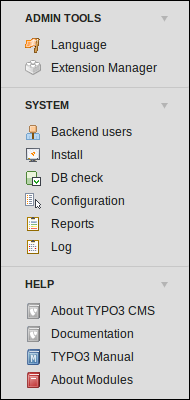
\includegraphics[width=0.35\linewidth]{Images/BackendChanges/AdminTools.png}
			\end{figure}
		\end{column}

	\end{columns}

\end{frame}

% ------------------------------------------------------------------------------
% Visual Appearance
% ------------------------------------------------------------------------------
% http://forge.typo3.org/issues/36017

\begin{frame}[fragile]
	\frametitle{Изменение во внутреннем интерфейсе}
	\framesubtitle{Внешний вид}

	\begin{itemize}
		\item \texttt{<h1>}-заголовки в основной области используют шрифт TYPO3 "Share"
	\end{itemize}

	\begin{figure}
		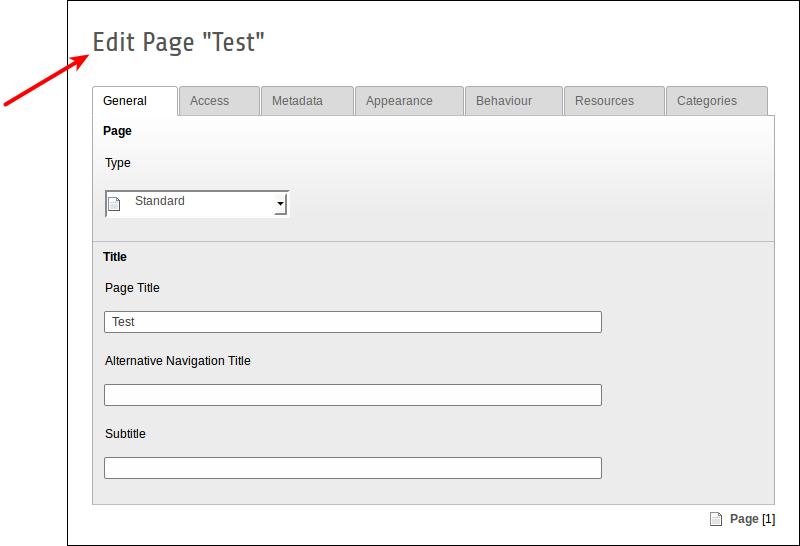
\includegraphics[width=0.6\linewidth]{Images/BackendChanges/ConsistantFont.png}
	\end{figure}

\end{frame}

% ------------------------------------------------------------------------------
% Visual Appearance
% ------------------------------------------------------------------------------
% http://forge.typo3.org/issues/41631

\begin{frame}[fragile]
	\frametitle{Изменение во внутреннем интерфейсе}
	\framesubtitle{Внешний вид}

	\begin{itemize}
		\item Новый значок для модуля "Отчёты"/"Reports"
	\end{itemize}

	\begin{figure}
		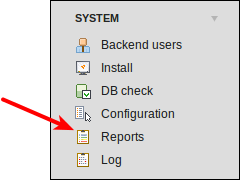
\includegraphics[width=0.35\linewidth]{Images/BackendChanges/ModuleReportsIcon.png}
	\end{figure}

\end{frame}

% ------------------------------------------------------------------------------
% Filelist: Drag&Drop File Upload
% ------------------------------------------------------------------------------
% http://forge.typo3.org/issues/47005

\begin{frame}[fragile]
	\frametitle{Изменение во внутреннем интерфейсе}
	\framesubtitle{Загрузка файлов перетаскиванием (1)}

	\begin{itemize}
		\item В списке файлов применен функционал HTML5 загрузки файлов перетаскиванием

	\end{itemize}

	\begin{figure}
		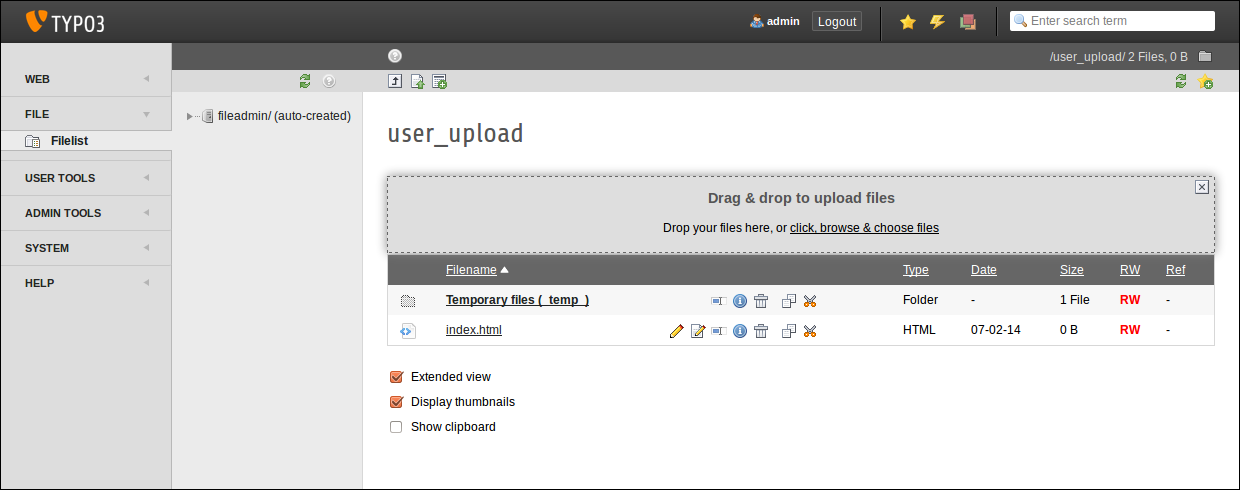
\includegraphics[width=0.95\linewidth]{Images/BackendChanges/DragDropFileUpload.png}
	\end{figure}

\end{frame}

% ------------------------------------------------------------------------------
% Drag&Drop File Upload Via Content Elements
% (slide added in March 2014)
% ------------------------------------------------------------------------------

\begin{frame}[fragile]
	\frametitle{Изменение во внутреннем интерфейсе}
	\framesubtitle{Загрузка файлов перетаскиванием (2)}

	\begin{itemize}
		\item ...и через элементы содержимого (кнопка: "Select \& upload files")

	\end{itemize}

	\begin{figure}
		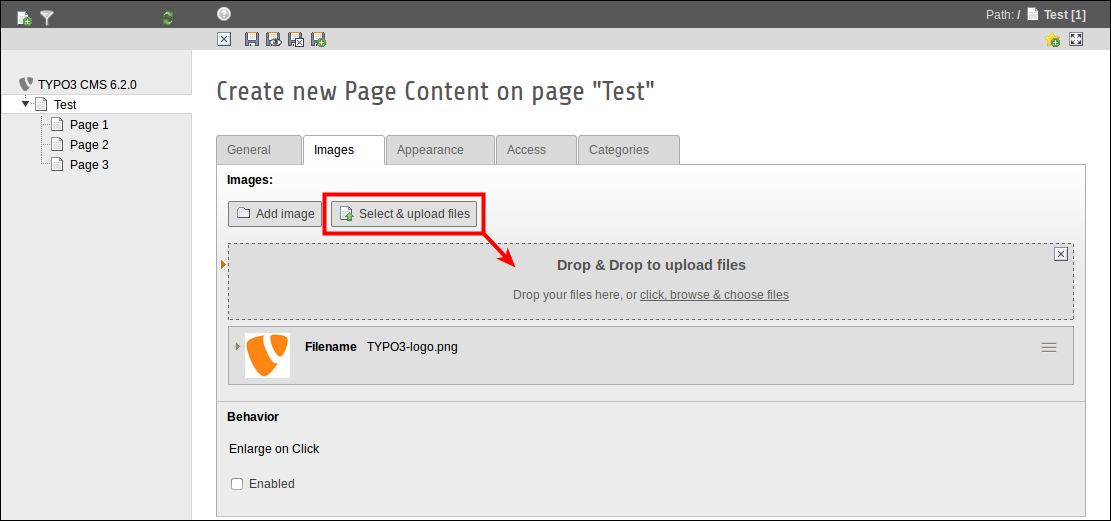
\includegraphics[width=0.95\linewidth]{Images/BackendChanges/SelectAndUploadFiles.png}
	\end{figure}

\end{frame}

% ------------------------------------------------------------------------------
% Backend Users
% ------------------------------------------------------------------------------
% http://forge.typo3.org/issues/43053

\begin{frame}[fragile]
	\frametitle{Изменение во внутреннем интерфейсе}
	\framesubtitle{Удобство: внутренние пользователи}

	\begin{itemize}
		\item Выводится имя пользователя и настоящее имя (первый столбец в режиме списка)
		\item Щёлкните по имени (пользователя) для его редактирования
		\item Удалена кнопка добавления в режиме списка

	\end{itemize}

	\begin{figure}
		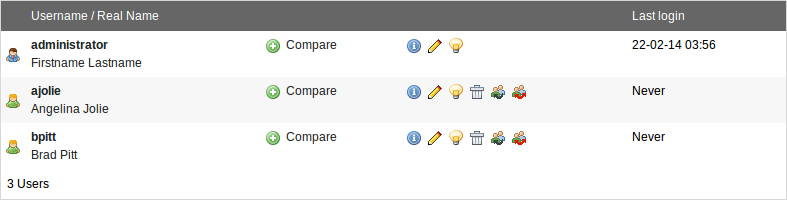
\includegraphics[width=0.95\linewidth]{Images/BackendChanges/BackendUserList.png}
	\end{figure}

\end{frame}

% ------------------------------------------------------------------------------
% Live Search
% ------------------------------------------------------------------------------
% http://forge.typo3.org/issues/35358

\begin{frame}[fragile]
	\frametitle{Изменение во внутреннем интерфейсе}
	\framesubtitle{Живой поиск}

	\begin{itemize}
		\item Подсказка в "живом поиске" показывает как UID, так и PID
		\item Если после поиска снова закрыть форму редактирования, то выводится режим списка для страницы (а не пустая страница)
	\end{itemize}

	\begin{figure}
		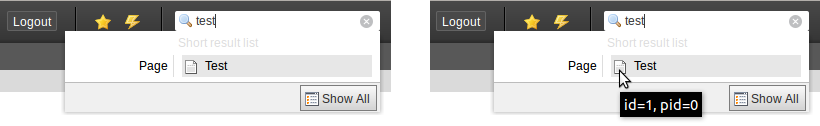
\includegraphics[width=0.8\linewidth]{Images/BackendChanges/LiveSearchTooltip.png}
	\end{figure}

\end{frame}

% ------------------------------------------------------------------------------
% Live Search
% ------------------------------------------------------------------------------

\begin{frame}[fragile]
	\frametitle{Изменение во внутреннем интерфейсе}
	\framesubtitle{Живой поиск}

	\begin{itemize}
		\item В TYPO3 < 6.2, для страниц учитывались лишь поля базы данных \texttt{title} и \texttt{uid}
		\item В TYPO3 >= 6.2, к поиску можно добавить поля \texttt{alias}\newline
			(требуется UserTSconfig: \texttt{options.pageTree.searchInAlias = 1})
	\end{itemize}

	\begin{figure}
		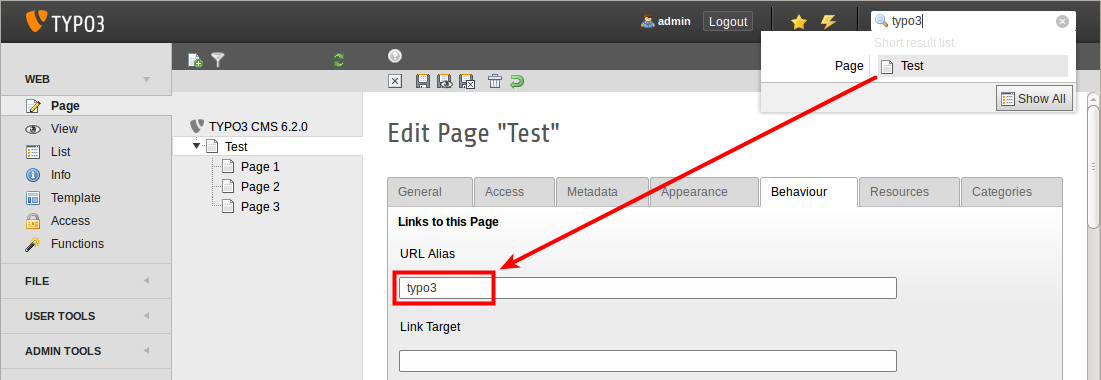
\includegraphics[width=0.95\linewidth]{Images/BackendChanges/LiveSearchInAlias.png}
	\end{figure}

\end{frame}

% ------------------------------------------------------------------------------
% File Abstraction Layer
% ------------------------------------------------------------------------------

\begin{frame}[fragile]
	\frametitle{Изменение во внутреннем интерфейсе}
	\framesubtitle{File Abstraction Layer}

	\begin{itemize}
		\item Название файла и заголовок выводятся в заголовке элемента FAL
	\end{itemize}

	\begin{figure}
		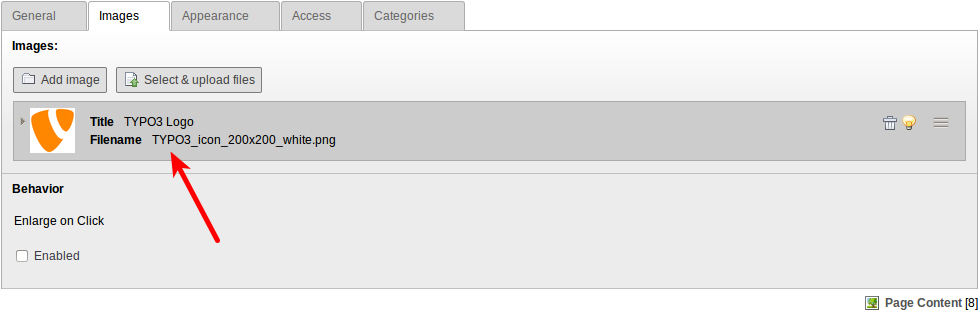
\includegraphics[width=0.95\linewidth]{Images/BackendChanges/FalTitleAndFilename.png}
	\end{figure}

\end{frame}

% ------------------------------------------------------------------------------
% File Abstraction Layer
% ------------------------------------------------------------------------------

\begin{frame}[fragile]
	\frametitle{Изменение во внутреннем интерфейсе}
	\framesubtitle{File Abstraction Layer (EXT:filemetadata)}

	\begin{itemize}
		\item EXT:filemetadata добавляет вкладки для вывода meta информации\newline
			\small(по умолчанию расширение не установлено)\normalsize
	\end{itemize}

	\begin{figure}
		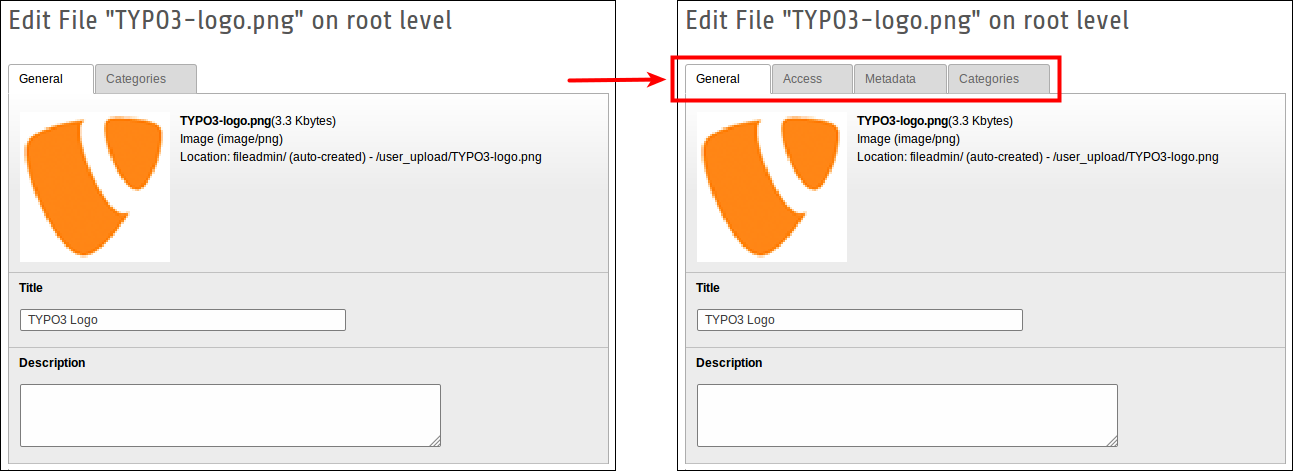
\includegraphics[width=0.95\linewidth]{Images/BackendChanges/FileMetaDataTabs.png}
	\end{figure}

\end{frame}

% ------------------------------------------------------------------------------
% File Abstraction Layer
% ------------------------------------------------------------------------------

\begin{frame}[fragile]
	\frametitle{Изменение во внутреннем интерфейсе}
	\framesubtitle{File Abstraction Layer (EXT:filemetadata)}

	\begin{figure}
		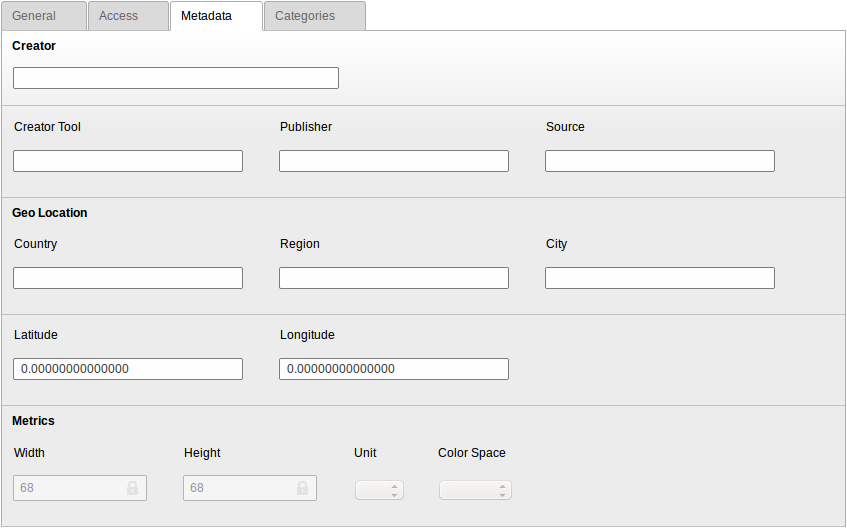
\includegraphics[width=0.8\linewidth]{Images/BackendChanges/FileMetaData.png}
	\end{figure}

\end{frame}


% ------------------------------------------------------------------------------
% File Abstraction Layer
% ------------------------------------------------------------------------------

\begin{frame}[fragile]
	\frametitle{Изменение во внутреннем интерфейсе}
	\framesubtitle{File Abstraction Layer}

	\begin{itemize}
		\item Теперь возможен перевод FAL meta данных на используемые на сайте языки
	\end{itemize}

	\begin{figure}
		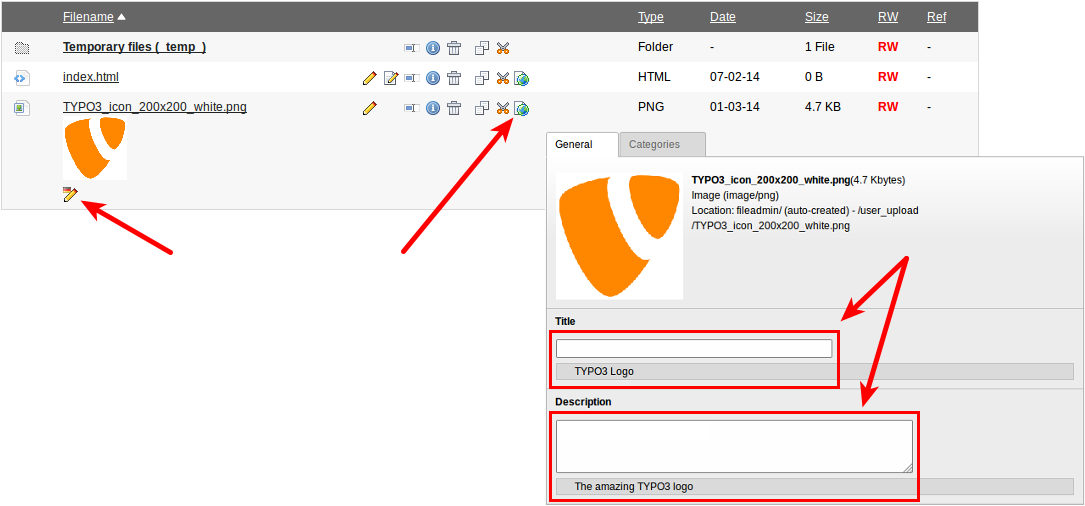
\includegraphics[width=0.95\linewidth]{Images/BackendChanges/FalTranslateMetaData.png}
	\end{figure}

\end{frame}

% ------------------------------------------------------------------------------
% Module: Documentation
% ------------------------------------------------------------------------------

\begin{frame}[fragile]
	\frametitle{Изменение во внутреннем интерфейсе}
	\framesubtitle{Модуль: документация (documentation)}

	\begin{columns}[T]

		\begin{column}{.5\textwidth}
			\begin{itemize}
				\item Модуль "Документация"/"Documentation" позволяет внутренним пользователям загружать и просматривать
				руководства
				\item По умолчанию модуль уже загружен в новых инсталяциях TYPO3
				\item В обновлённых инсталяциях TYPO3 для установки "Документация"/"Documentation" используйте модуль
				управления расширениями
				\item Функция "Управление документацией"/"Manage Documentation" загружает руководства (см. рисунок)
			\end{itemize}
		\end{column}

		\begin{column}{.5\textwidth}
			\begin{figure}\vspace*{-0.4cm}
				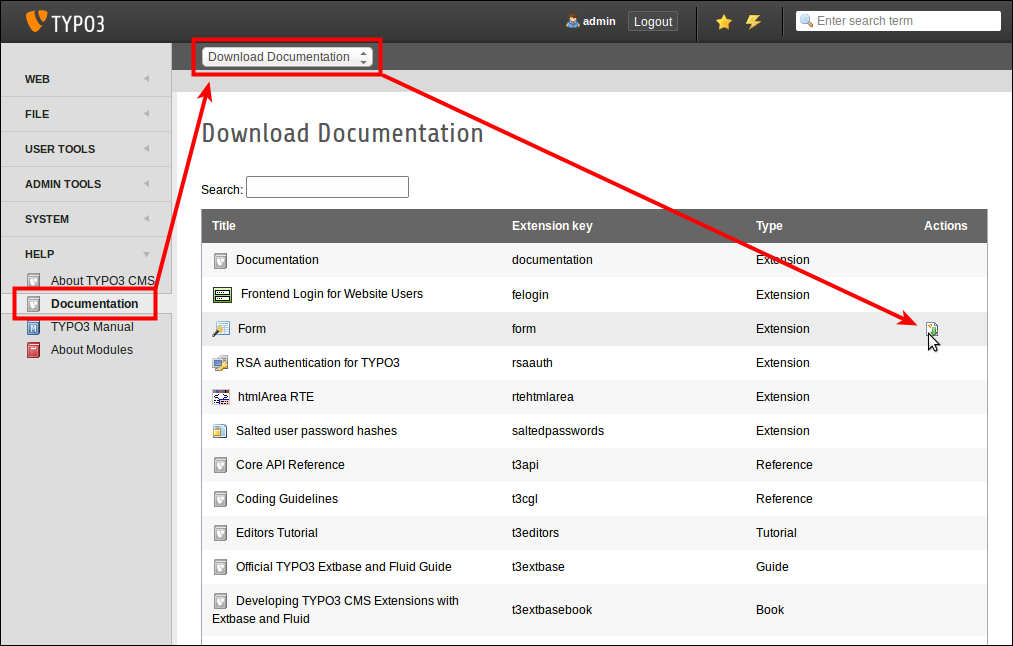
\includegraphics[width=1\linewidth]{Images/BackendChanges/DownloadDocumentation.png}
			\end{figure}
		\end{column}

	\end{columns}

\end{frame}

% ------------------------------------------------------------------------------
% Module: Documentation
% ------------------------------------------------------------------------------

\begin{frame}[fragile]
	\frametitle{Изменение во внутреннем интерфейсе}
	\framesubtitle{Модуль: документация (documentation)}

	\begin{itemize}
		\item Функция "Показать документацию"/"Show Documentation" выводит загруженные документы
	\end{itemize}

	\begin{figure}
		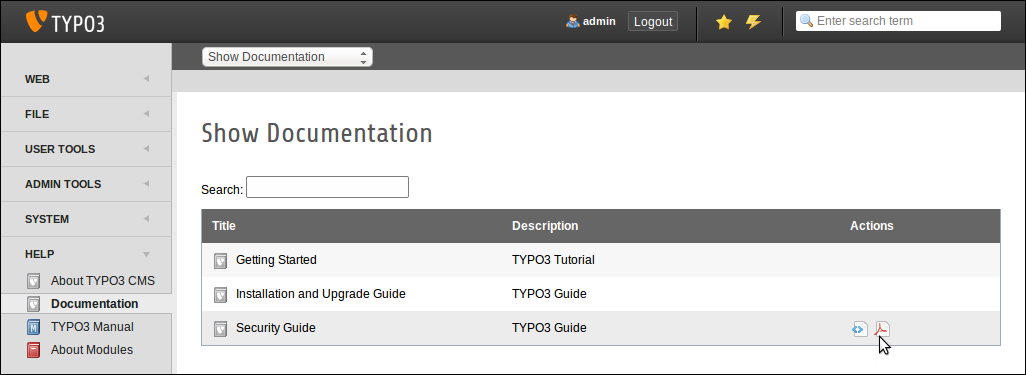
\includegraphics[width=0.95\linewidth]{Images/BackendChanges/ShowDocumentation.png}
	\end{figure}

\end{frame}

% ------------------------------------------------------------------------------
% Removed: TypoScript Help
% ------------------------------------------------------------------------------
% http://forge.typo3.org/issues/47931

\begin{frame}[fragile]
	\frametitle{Изменение во внутреннем интерфейсе}
	\framesubtitle{Удалено: Справка TypoScript/TypoScript Help}

 	\begin{itemize}
		\item EXT:tsconfig\_help ("TSconfig Quick Reference") удален\newline
			\small(устаревшая информация, не обновляемая со времен TYPO3 CMS 4.1)
	\end{itemize}

	\begin{figure}
		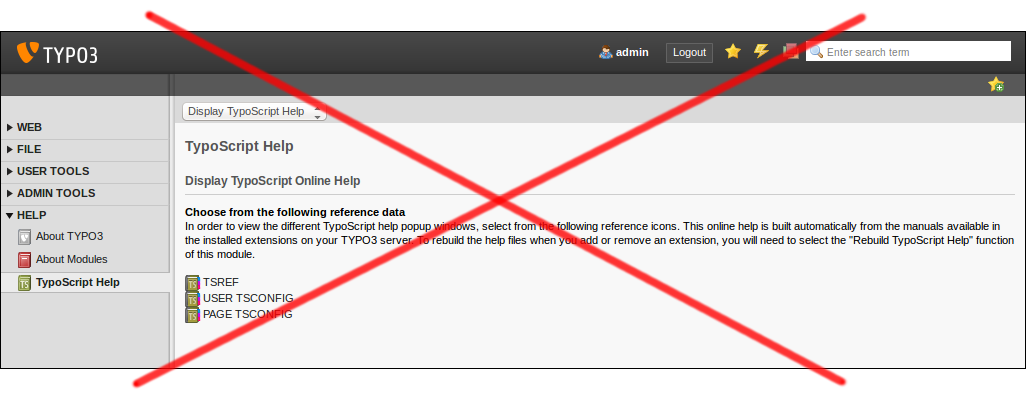
\includegraphics[width=0.95\linewidth]{Images/BackendChanges/TypoScriptHelpRemovedCrossed.png}
	\end{figure}

\end{frame}


% ------------------------------------------------------------------------------
% Scheduler
% ------------------------------------------------------------------------------

\begin{frame}[fragile]
	\frametitle{Изменение во внутреннем интерфейсе}
	\framesubtitle{Планировщик/Scheduler}

	\begin{itemize}
		\item Удаление запланированных задач в режиме правки\newline
			\small(в TYPO3 < 6.2, функция удаления была доступна лишь в режиме списка)\normalsize
	\end{itemize}

	\begin{figure}
		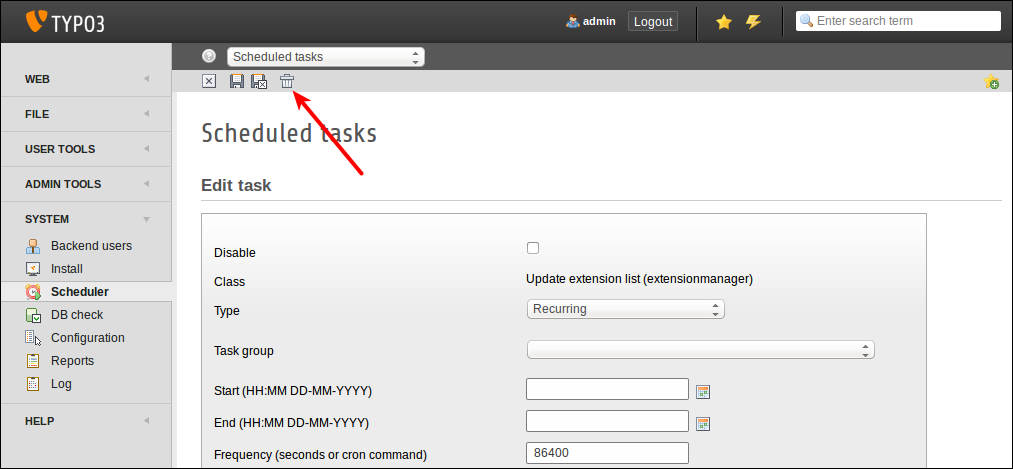
\includegraphics[width=0.95\linewidth]{Images/BackendChanges/DeleteSchedulerTaskInEditView.png}
	\end{figure}

\end{frame}

% ------------------------------------------------------------------------------
% Scheduler
% ------------------------------------------------------------------------------

\begin{frame}[fragile]
	\frametitle{Изменение во внутреннем интерфейсе}
	\framesubtitle{Планировщик/Scheduler}

	\begin{itemize}
		\item К запланированной задаче можно прикрепить описание, которое выводится в виде подзаголовка в режиме списка,
		либо как подсказка (на следующем слайде)
	\end{itemize}

	\begin{figure}
		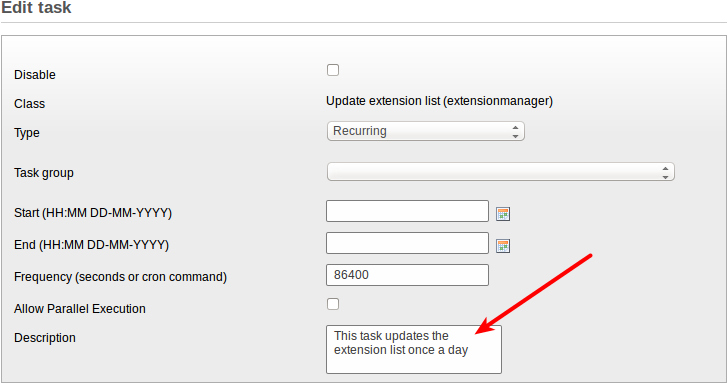
\includegraphics[width=0.7\linewidth]{Images/BackendChanges/SchedulerTaskDescription.png}
	\end{figure}

\end{frame}

% ------------------------------------------------------------------------------
% Scheduler
% ------------------------------------------------------------------------------

\begin{frame}[fragile]
	\frametitle{Изменение во внутреннем интерфейсе}
	\framesubtitle{Планировщик/Scheduler}

	\begin{itemize}
		\item Описание задачи в виде подзаголовка\newline
			\small(необходимо включение в настройке расширения)\normalsize
	\end{itemize}

	\begin{figure}
		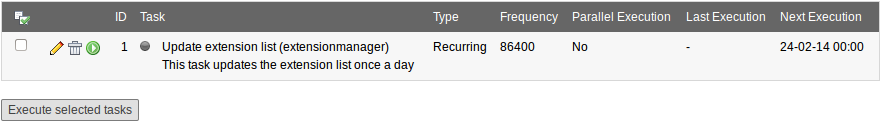
\includegraphics[width=0.95\linewidth]{Images/BackendChanges/SchedulerTaskDescriptionAsSubheader.png}
	\end{figure}


	\begin{itemize}
		\item Описание задачи в виде подсказки ("hover")
	\end{itemize}

	\begin{figure}
		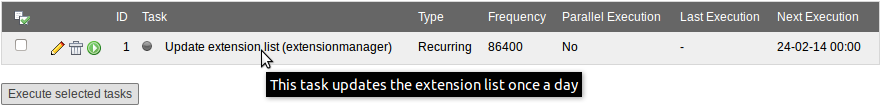
\includegraphics[width=0.95\linewidth]{Images/BackendChanges/SchedulerTaskDescriptionAsTooltip.png}
	\end{figure}

\end{frame}

% ------------------------------------------------------------------------------
% Scheduler
% ------------------------------------------------------------------------------

\begin{frame}[fragile]
	\frametitle{Изменение во внутреннем интерфейсе}
	\framesubtitle{Планировщик/Scheduler}

	\begin{itemize}
		\item Теперь возможна группировка планируемых задач
		\item Добавляйте записи "группа плановых задач"/"scheduler task group" на корневую страницу (UID: 0) и выбирайте группу
		 в задаче
	\end{itemize}

	\begin{figure}
		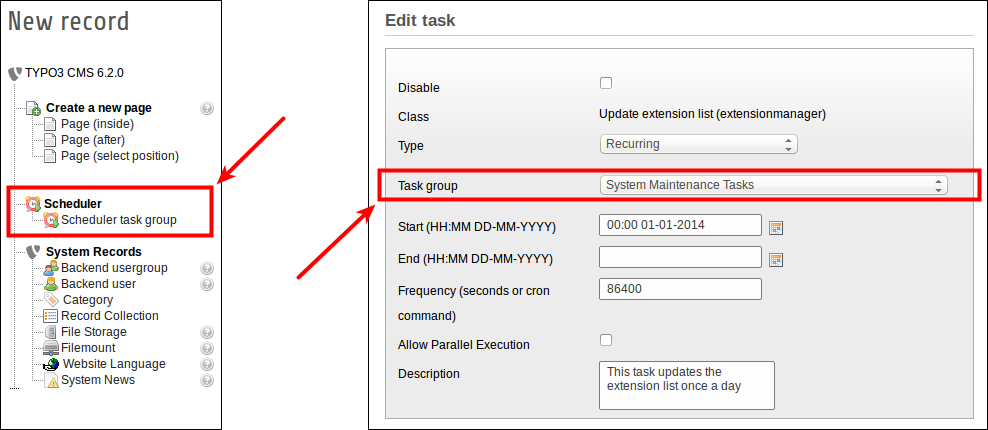
\includegraphics[width=0.85\linewidth]{Images/BackendChanges/SchedulerTaskGroup.png}
	\end{figure}

\end{frame}

% ------------------------------------------------------------------------------
% System Extension: Form
% ------------------------------------------------------------------------------
% http://forge.typo3.org/issues/38094

\begin{frame}[fragile]
	\frametitle{Изменение во внутреннем интерфейсе}
	\framesubtitle{Системное расширение: Формы/Form}

		\begin{columns}[T]

    		\begin{column}{.5\textwidth}
				\begin{itemize}
					\item Новая пост обработка для cObject FORM: \textbf{redirect}\newline
						(перенаправление после подтверждения формы)
					\item Значение анализируется в \texttt{typolink} (функция TypoScript),\newline
						то есть значение может быть и ID страницы, и URL
				\end{itemize}
    		\end{column}

    		\begin{column}{.5\textwidth}
    			\begin{figure}\vspace*{-0.4cm}
    				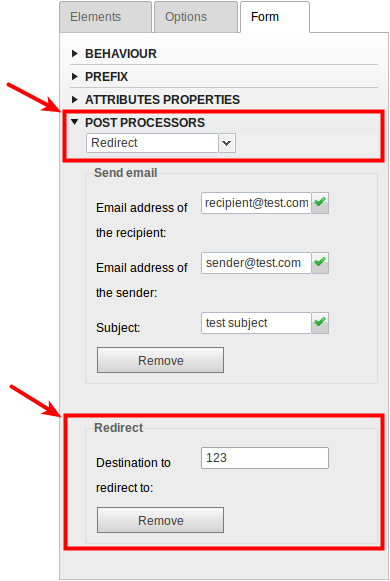
\includegraphics[width=0.65\linewidth]{Images/BackendChanges/FormRedirectPostProcessor.png}
    			\end{figure}
    		\end{column}

    	\end{columns}

\end{frame}

% ------------------------------------------------------------------------------
% Module: List
% ------------------------------------------------------------------------------
% http://forge.typo3.org/issues/49810

\begin{frame}[fragile]
	\frametitle{Изменение во внутреннем интерфейсе}
	\framesubtitle{Модуль Список/List}

	\begin{itemize}
		\item Дополнительные столбцы "UID" и "PID" в режиме списка для не администраторов/admins
	\end{itemize}

	\begin{figure}
		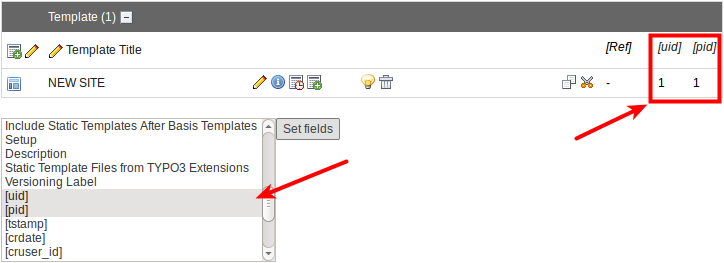
\includegraphics[width=0.95\linewidth]{Images/BackendChanges/AdditionalColumnsInListModule.png}
	\end{figure}

\end{frame}

% ------------------------------------------------------------------------------
% File Abstraction Layer
% ------------------------------------------------------------------------------
% http://forge.typo3.org/issues/50827
% http://forge.typo3.org/issues/51097

\begin{frame}[fragile]
	\frametitle{Изменение во внутреннем интерфейсе}
	\framesubtitle{File Abstraction Layer}

	\begin{itemize}
		\item Если при индексации обнаружен файл с ошибкой, выводится сообщение и устанавливается флаг для записи в БД
		\item Это отображается и в модуле "Отчеты"/"Reports"
		\item Если же файл снова появляется, сообщение и флаг сбрасываются
	\end{itemize}

	\begin{columns}[T]

		\begin{column}{.5\textwidth}
			\begin{figure}
				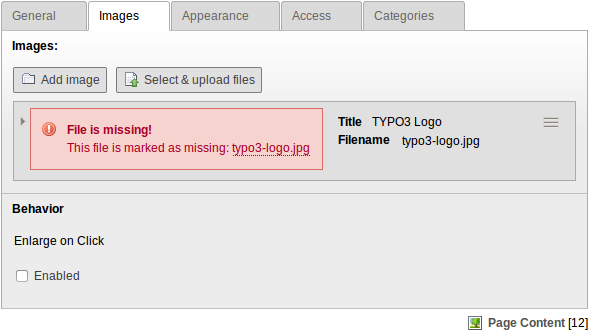
\includegraphics[width=0.95\linewidth]{Images/BackendChanges/FalMissingFileContentElement.png}
			\end{figure}
		\end{column}

		\begin{column}{.5\textwidth}
			\begin{figure}
				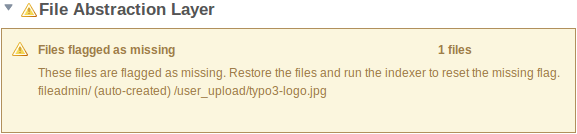
\includegraphics[width=0.95\linewidth]{Images/BackendChanges/FalMissingFileReportsModule.png}
			\end{figure}
		\end{column}

	\end{columns}

\end{frame}

% ------------------------------------------------------------------------------
% Menu/Sitemap: Categories-based Menus
% ------------------------------------------------------------------------------
% http://forge.typo3.org/issues/51161

\begin{frame}[fragile]
	\frametitle{Изменение во внутреннем интерфейсе}
	\framesubtitle{Меню категорий (1)}

	\begin{itemize}
		\item Элемент содержимого "Меню/Карта сайта"/"Menu/Sitemap" теперь может создавать меню категорий
	\end{itemize}

	\begin{figure}
		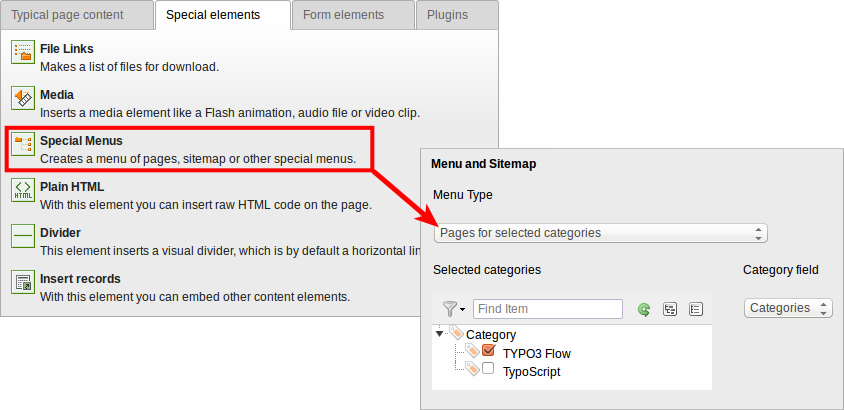
\includegraphics[width=0.8\linewidth]{Images/BackendChanges/CategoryBasedMenus.png}
	\end{figure}

\end{frame}

% ------------------------------------------------------------------------------
% Menu/Sitemap: Category-based Menus
% (slide added in March 2014)
% ------------------------------------------------------------------------------


\begin{frame}[fragile]
	\frametitle{Изменение во внутреннем интерфейсе}
	\framesubtitle{Меню категорий (2)}

	\begin{itemize}
		\item Другой тип нового меню: "\underline{Элементы содержимого} из выбранных категорий"
	\end{itemize}

	\begin{figure}
		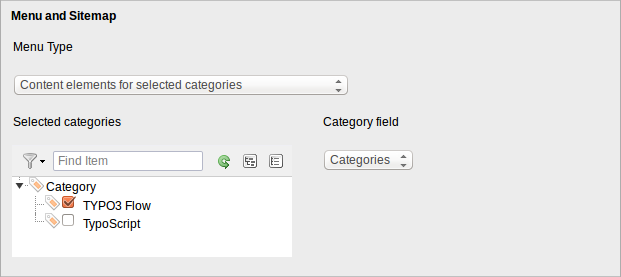
\includegraphics[width=0.6\linewidth]{Images/BackendChanges/ContentElementsForSelectedCategories.png}
	\end{figure}

\end{frame}

% ------------------------------------------------------------------------------
% Sorting Categories
% ------------------------------------------------------------------------------
% http://forge.typo3.org/issues/51590

\begin{frame}[fragile]
	\frametitle{Изменение во внутреннем интерфейсе}
	\framesubtitle{Упорядочивание категорий}

 	\begin{itemize}
		\item Теперь категории можно упорядочить\newline
			\small(в TYPO3 < 6.2, категории всегда выводились по алфавиту)\normalsize
	\end{itemize}

	\begin{figure}
		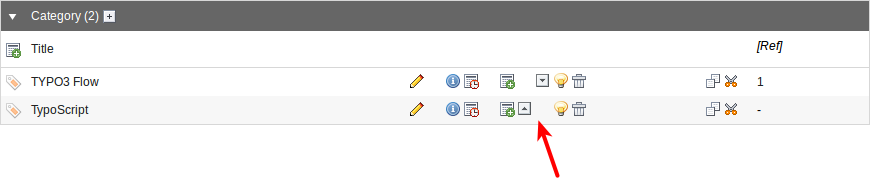
\includegraphics[width=0.95\linewidth]{Images/BackendChanges/CategorySorting.png}
	\end{figure}

\end{frame}

% ------------------------------------------------------------------------------
% Category Visibility
% ------------------------------------------------------------------------------
% http://forge.typo3.org/issues/52718

\begin{frame}[fragile]
	\frametitle{Изменение во внутреннем интерфейсе}
	\framesubtitle{Видимость категорий}

 	\begin{itemize}
		\item Для внутренних пользователей/групп можно ограничить видимость категорий
		users/groups
	\end{itemize}

	\begin{figure}
		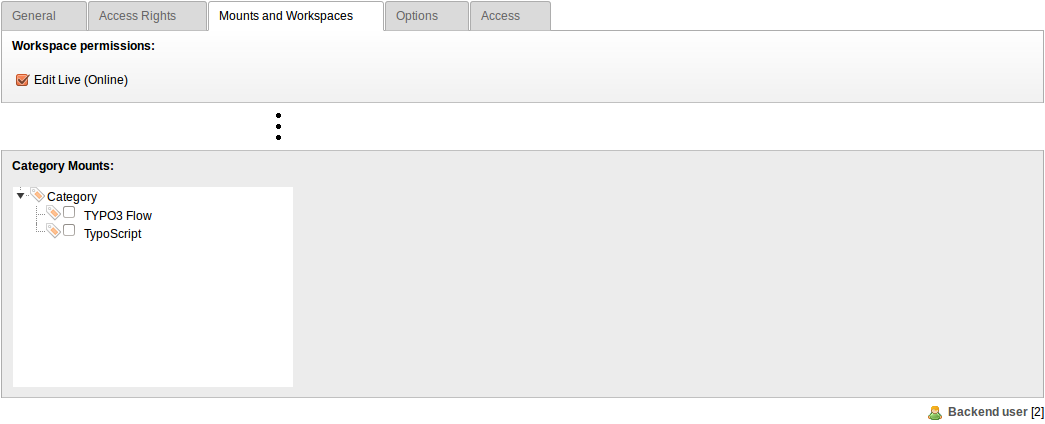
\includegraphics[width=0.95\linewidth]{Images/BackendChanges/CategoryVisibility.png}
	\end{figure}

\end{frame}

% ------------------------------------------------------------------------------
% "New Content" icon always visible
% ------------------------------------------------------------------------------
% http://forge.typo3.org/issues/48938
% http://forge.typo3.org/issues/51480

\begin{frame}[fragile]
	\frametitle{Изменение во внутреннем интерфейсе}
	\framesubtitle{Удобство}

 	\begin{itemize}
		\item Если столбец пуст, всегда выводиться значок "добавить содержимое"/"new content"\newline
			\small(это помогает редакторам понять, что они могут сделать)\normalsize
	\end{itemize}

	\begin{figure}
		\includegraphics[width=0.95\linewidth]{Images/BackendChanges/NewContentIconAlwaysVisible.png}
	\end{figure}

\end{frame}

% ------------------------------------------------------------------------------
% Module "Functions": Hide In Menus
% ------------------------------------------------------------------------------
% http://forge.typo3.org/issues/51017

\begin{frame}[fragile]
	\frametitle{Изменение во внутреннем интерфейсе}
	\framesubtitle{Функции}

    \begin{itemize}
		\item При создании нескольких страниц в модуле "функции"/"functions", новый флажок позволяет редакторам скрыть
		эти страницы в меню
		\smallОчень полезно при создании множества страниц за раз\normalsize
	\end{itemize}

	\begin{figure}
		\includegraphics[width=0.85\linewidth]{Images/BackendChanges/CreateMultiplePagesHideInMenu.png}
	\end{figure}

\end{frame}

% ------------------------------------------------------------------------------
% Extension Manager: Upload Extensions
% ------------------------------------------------------------------------------
% http://forge.typo3.org/issues/51776
% http://forge.typo3.org/issues/51437

\begin{frame}[fragile]
	\frametitle{Изменение во внутреннем интерфейсе}
	\framesubtitle{Управление расширениями}

 	\begin{itemize}
		\item Загрузка расширений посредством функции "Получить расширение"/"Get Extensions"
	\end{itemize}

	\begin{figure}
		\includegraphics[width=0.95\linewidth]{Images/BackendChanges/UploadExtension.png}
	\end{figure}

\end{frame}

% ------------------------------------------------------------------------------
% Recycler
% ------------------------------------------------------------------------------
% http://forge.typo3.org/issues/52324

\begin{frame}[fragile]
	\frametitle{Изменение во внутреннем интерфейсе}
	\framesubtitle{Корзина}

 	\begin{itemize}
		\item Записи в корзине можно упорядочить по времени\newline
			\small(что помогает пользователям решить, какую запись нужно восстановить)\normalsize
	\end{itemize}

	\begin{figure}
		\includegraphics[width=0.95\linewidth]{Images/BackendChanges/RecyclerSortRecord.png}
	\end{figure}

\end{frame}

% ------------------------------------------------------------------------------
% File/Directory Permissions
% ------------------------------------------------------------------------------

\begin{frame}[fragile]
	\frametitle{Изменение во внутреннем интерфейсе}
	\framesubtitle{Разрешения для Файлов/Директорий}

    \begin{itemize}
		\item Гораздо более детальная настройка разрешений для файлов/директория для внутренних пользователей/групп
			\begingroup\color{typo3red}\textbf{(1)}\endgroup
		\item Возможно, начиная с TYPO3 6.0, но только через UserTSconfig
			\begingroup\color{typo3red}\textbf{(2)}\endgroup
	\end{itemize}

	\begin{figure}
		\includegraphics[width=0.75\linewidth]{Images/BackendChanges/FileAndDirectoryPermissions.png}
	\end{figure}

\end{frame}

% ------------------------------------------------------------------------------
% OpenID
% ------------------------------------------------------------------------------

\begin{frame}[fragile]
	\frametitle{Изменение во внутреннем интерфейсе}
	\framesubtitle{OpenID (1)}

 	\begin{itemize}
		\item OpenID для авторизации внутренних пользователей можно настроить через мастер
		\item Для этого потребуется установить EXT:openid (системное расширение)
	\end{itemize}

	\begin{figure}
		\includegraphics[width=0.95\linewidth]{Images/BackendChanges/OpenIdWizard.png}
	\end{figure}

\end{frame}

% ------------------------------------------------------------------------------
% OpenID
% ------------------------------------------------------------------------------

\begin{frame}[fragile]
	\frametitle{Изменение во внутреннем интерфейсе}
	\framesubtitle{OpenID (2)}

 	\begin{itemize}
		\item OpenID для авторизации внутренних пользователей можно настроить через мастер
		\item Для этого потребуется установить EXT:openid (системное расширение)
	\end{itemize}

	\begin{figure}
		\includegraphics[width=0.8\linewidth]{Images/BackendChanges/OpenIdLogin.png}
	\end{figure}

 	\begin{itemize}
		\item Дополнительно об OpenID:\newline
			\small\url{http://openid.net}\normalsize
	\end{itemize}


\end{frame}

% ------------------------------------------------------------------------------
% Workspaces
% ------------------------------------------------------------------------------
% http://forge.typo3.org/issues/50223
% http://forge.typo3.org/issues/50224

\begin{frame}[fragile]
	\frametitle{Изменение во внутреннем интерфейсе}
	\framesubtitle{Рабочие области/Workspaces}

 	\begin{itemize}
		\item Редакторы/пользователи могут определять кого извещать, без ограничения со стороны системы
		\item Вкладка "Все"/"All" теперь видна для \underline{всех} пользователей
	\end{itemize}

	\begin{figure}
		\includegraphics[width=0.95\linewidth]{Images/BackendChanges/WorkspacesTabAll.png}
	\end{figure}

\end{frame}

% ------------------------------------------------------------------------------



% ------------------------------------------------------------------------------
% Chapter 4: TypoScript
% ------------------------------------------------------------------------------

% ------------------------------------------------------------------------------
% TYPO3 CMS 6.2 LTS - What's New - Chapter "TypoScript" (English Version)
%
% @author	Michael Schams <schams.net>
% @license	Creative Commons BY-NC-SA 3.0
% @link		http://typo3.org/download/release-notes/whats-new/
% @language	English
% ------------------------------------------------------------------------------
% Chapter: TypoScript
% ------------------------------------------------------------------------------
\section{TSconfig \& TypoScript}
\begin{frame}[fragile]
	\frametitle{TSconfig \& TypoScript}

	\begin{center}\huge{Rozdział 4:}\end{center}
	\begin{center}\huge{\color{typo3darkgrey}\textbf{TSconfig \& TypoScript}}\end{center}

\end{frame}

% ------------------------------------------------------------------------------
% Include TypoScript
% ------------------------------------------------------------------------------
% http://forge.typo3.org/issues/34621

\begin{frame}[fragile]
	\frametitle{TSconfig \& TypoScript}
	\framesubtitle{Dołączanie TypoScript-u}

	\begin{itemize}
		\item Dołącz wszystkie pliki TypoScript-u z folderu (rekurencyjnie)

			\lstinline!<INCLUDE_TYPOSCRIPT: source="DIR:directory">!
			\lstinline!<INCLUDE_TYPOSCRIPT: source="DIR:EXT:myextension/res/setup">!

		\item Kolejność w której dołączane są pliki:\newline
			alfabetycznie, najpierw pliki a później foldery
		\item Ograniczenia plików, które będą dołączone przez dodanie \texttt{rozszerzenia="..."}

			\lstinline!<INCLUDE_TYPOSCRIPT: source="DIR:directory" extensions="ts">!

		\item Domyślnie, tylko pliki z rozszerzeniami ts, t3, t3s, t3c, txt mogą być dołączone
		\item Lista ta jest konfigurowalna (Instalator):\newline
			\texttt{\$TYPO3\_CONF\_VARS['SYS']['tsfile\_ext']}
	\end{itemize}

\end{frame}

% ------------------------------------------------------------------------------
% Include TypoScript
% ------------------------------------------------------------------------------
% http://forge.typo3.org/issues/52018

\begin{frame}[fragile]
	\frametitle{TSconfig \& TypoScript}
	\framesubtitle{Dołączanie TypoScript-u}

	\begin{itemize}
		\item Ścieżki względne mogą być wpisane w \texttt{INCLUDE\_TYPOSCRIPT},\newline
			jeśli włączanie jest wywołane rekurencyjnie z pliku
		\item Pierwsze dołączenie \textbf{musi być} bezwzględne
		\item \texttt{./} odzwierciedla aktualny folder ostatniego dołączenia
		\item \texttt{../} odzwierciedla folder rodzica folderu ostatniego dołączenia
		\item Przykłady:

			\lstinline!<INCLUDE_TYPOSCRIPT: source="FILE:directory/typoscript/setup.ts">!
			\lstinline!<INCLUDE_TYPOSCRIPT: source="FILE:./filename.ts">!
			\lstinline!<INCLUDE_TYPOSCRIPT: source="FILE:../filename.ts">!
			\lstinline!<INCLUDE_TYPOSCRIPT: source="FILE:../directory/filename.ts">!

	\end{itemize}

\end{frame}

% ------------------------------------------------------------------------------
% stdWrap for strPad
% ------------------------------------------------------------------------------
% http://forge.typo3.org/issues/43604

\begin{frame}[fragile]
	\frametitle{TSconfig \& TypoScript}
	\framesubtitle{strPad}

	\begin{itemize}
		\item Opcja \texttt{stdWrap} została dodana do właściwości \texttt{strPad} 

			\begin{lstlisting}
				page = PAGE
				page.10 = TEXT
				page.10 {
				  value = Hello World!
				  strPad {
				    length = 5
				    length {
				      current = 1
				      setCurrent.data = TSFE:page|uid
				      setCurrent.wrap = | + 80
				      prioriCalc = 1
				    }
				    padWith = .
				  }
				}
			\end{lstlisting}

	\end{itemize}

\end{frame}

% ------------------------------------------------------------------------------
% stdWrap for _DEFAULT_PI_VARS
% ------------------------------------------------------------------------------
% http://forge.typo3.org/issues/22045
% http://forge.typo3.org/issues/49314

\begin{frame}[fragile]
	\frametitle{TSconfig \& TypoScript}
	\framesubtitle{\_DEFAULT\_PI\_VARS}

	\begin{itemize}
		\item \texttt{stdWrap} zostało dodane do \texttt{\_DEFAULT\_PI\_VARS}
		\item \texttt{\_DEFAULT\_PI\_VARS} jest używane do ustawiania domyślnej wartości dla piVars (zmienne GET/POST jako rozszerzenie)

		\item TYPO3 < 6.2
			\begin{lstlisting}
				plugin.tt_news._DEFAULT_PI_VARS {
				  year = 2013
				}
			\end{lstlisting}

		\item TYPO3 >= 6.2
			\begin{lstlisting}
				plugin.tt_news._DEFAULT_PI_VARS {
				  year.stdWrap.data = date:Y
				}
			\end{lstlisting}

	\end{itemize}

\end{frame}

% ------------------------------------------------------------------------------
% Debug Register and Page
% ------------------------------------------------------------------------------
% http://forge.typo3.org/issues/49478

\begin{frame}[fragile]
	\frametitle{TSconfig \& TypoScript}
	\framesubtitle{Debugowanie wyjścia}

	\begin{columns}[T]

		\begin{column}{.6\textwidth}
			\begin{itemize}
				\item Debugowanie wyjścia dla rejestru i zmiennych na stronie:\newline
					\texttt{\$GLOBALS['TSFE']->register}\newline
					\texttt{\$GLOBALS['TSFE']->page}

				\item Przykłady:

					\begin{lstlisting}
						10 = LOAD_REGISTER
						10.variable = value
					\end{lstlisting}

					\begin{lstlisting}
						20 = TEXT
						20.data = debug:register
					\end{lstlisting}

					\begin{lstlisting}
						30 = TEXT
						30.data = debug:page
					\end{lstlisting}

			\end{itemize}
		\end{column}

		\begin{column}{.4\textwidth}
			\begin{figure}\vspace*{-0.4cm}
				\includegraphics[width=0.6\linewidth]{Images/TypoScript/DebugRegisterAndPage.png}
			\end{figure}
		\end{column}

	\end{columns}

\end{frame}

% ------------------------------------------------------------------------------
% File Links: "register:titleText" and "register:altText"
% ------------------------------------------------------------------------------
% http://forge.typo3.org/issues/44182

\begin{frame}[fragile]
	\frametitle{TSconfig \& TypoScript}
	\framesubtitle{Linki do plików}

	\begin{itemize}
		\item Odnośniki do plików oferują opis, tytuł tekstu i alternatywną etykietę dla każdego pliku.
			Wszystkie trzy mogą być dostępne z rejestru:

			\begin{itemize}
				\item \texttt{register:description}
				\item \texttt{register:titleText}
				\item \texttt{register:altText}
			\end{itemize}

		\item Przykład:

			\begin{lstlisting}
				# filelinks
				tt_content.uploads.20 {
				  # link description instead of filename
				  labelStdWrap.data = register:description
				  # output alternative text
				  itemRendering.20.data = register:titleText
				}
			\end{lstlisting}

	\end{itemize}

\end{frame}

% ------------------------------------------------------------------------------
% stdWrap replacement: add optionSplit-support
% ------------------------------------------------------------------------------
% http://forge.typo3.org/issues/42287

\begin{frame}[fragile]
	\frametitle{TSconfig \& TypoScript}
	\framesubtitle{funkcja stdWrap : wymiana (1)}

	\begin{itemize}
		\item Opcja \texttt{replace} w \texttt funkcji-{stdWrap} \texttt{replacement}\newline
			wspiera teraz \texttt{optionSplit}

		\item Przykład 1:

			\begin{lstlisting}
				10 = TEXT
				10.value = TYPO3_inspires_people_to_share
				10.replacement.10 {
				  search = _
				  replace = 1 || 2 || 3
				  useOptionSplitReplace = 1
				}
			\end{lstlisting}

			Wyjście:\newline
				\texttt{TYPO31inspires2people3to3share}

	\end{itemize}

\end{frame}

% ------------------------------------------------------------------------------
% stdWrap replacement: add optionSplit-support
% ------------------------------------------------------------------------------
% http://forge.typo3.org/issues/42287

\begin{frame}[fragile]
	\frametitle{TSconfig \& TypoScript}
	\framesubtitle{funkcja stdWrap : wymiana (2)}

	\begin{itemize}
		\item Opcja \texttt{replace} w \texttt funkcji-{stdWrap} \texttt{replacement}\newline
			wspiera teraz \texttt{optionSplit}

		\item Przykład 2:

			\begin{lstlisting}
				10 = TEXT
				10.value = TYPO3 inspires people to share
				10.replacement.10 {
				  search = #(TYPO3|people|share)#i
				  replace = ${1} CMS || all ${1} || collaborate and ${1}
				  useOptionSplitReplace = 1
				  useRegExp = 1
				}
			\end{lstlisting}

			Wyjście:\newline
				\texttt{TYPO3 CMS inspiruje wszystkich ludzi do współpracy i dzielenia się}

	\end{itemize}

\end{frame}

% ------------------------------------------------------------------------------
% Register values in FilesContentObject
% ------------------------------------------------------------------------------
% http://forge.typo3.org/issues/49480

\begin{frame}[fragile]
	\frametitle{TSconfig \& TypoScript}
	\framesubtitle{cObject FILE}

	\begin{itemize}
		\item Dwa rejestry dodane do PLIKÓW cObject:\newline
			\texttt{FILE\_NUM\_CURRENT} and \texttt{FILES\_COUNT}

		\item Przykład:

			\lstset{
				basicstyle=\tiny\ttfamily
			}

			\begin{lstlisting}
				10 = FILES
				10 {
				  references {
				    table = tt_news
				    uid.field = uid
				    fieldName = media
				  }
				  renderObj = COA
				  renderObj {
				    10 = TEXT
				    10.value = Renders first file twice
				    10.if.isFalse.data = register:FILE_NUM_CURRENT
				    20 = TEXT
				    20.value = file {register:FILE_NUM_CURRENT} of {register:FILES_COUNT}
				    20.insertData = 1
				  }
				}
			\end{lstlisting}

	\end{itemize}

\end{frame}

% ------------------------------------------------------------------------------
% Category Menu In TypoScript
% ------------------------------------------------------------------------------
% http://forge.typo3.org/issues/51161

\begin{frame}[fragile]
	\frametitle{TSconfig \& TypoScript}
	\framesubtitle{Menu kategorii}

	\begin{itemize}
		\item Generowanie menu z kategoriami w TypoScript-cie

		\item Przykład:

			\lstset{
				basicstyle=\tiny\ttfamily
			}

			\begin{lstlisting}
				page.20 = HMENU
				page.20 {
				  special = categories
				  special {
				    # comma-separated list of categories
				    value = 1
				    # sort by title (stdWrap)
				    sorting = title
				    # sorting "asc" or "desc" (stdWrap)
				    order = desc
				    1 = TMENU
				    1.NO {
				      allWrap = <li> | </li>
				    }
				  }
				}
			\end{lstlisting}

	\end{itemize}

\end{frame}

% ------------------------------------------------------------------------------
% cObject RECORDS with category support
% (slide added in March 2014)
% ------------------------------------------------------------------------------

\begin{frame}[fragile]
	\frametitle{TSconfig \& TypoScript}
	\framesubtitle{Kategoria dostępu}

	\begin{itemize}
		\item Właściwość \texttt{categories} zezwala na dostęp do kategorii \newline
			dla REKORDÓW cObject

		\item Przykład:

			\lstset{
				basicstyle=\tiny\ttfamily
			}

			\begin{lstlisting}
				# menu of categorized content elements
				categorized_content = RECORDS
				categorized_content {
				  categories.field = selected_categories
				  categories.relation.field = category_field
				  tables = tt_content
				  conf.tt_content = TEXT
				  conf.tt_content {
				    field = header
				    typolink.parameter = {field:pid}#{field:uid}
				    typolink.parameter.insertData = 1
				    wrap = <li>|</li>
				  }
				  wrap = <ul>|</ul>
				}
			\end{lstlisting}

	\end{itemize}

\end{frame}

% ------------------------------------------------------------------------------
% Category Menu In TypoScript
% ------------------------------------------------------------------------------
% http://forge.typo3.org/issues/51782

\begin{frame}[fragile]
	\frametitle{TSconfig \& TypoScript}
	\framesubtitle{Pliki CSS i JavaScript}

	\begin{itemize}
		\item \texttt{splitChar} teraz może być zdefiniowany dla wszystkich właściwości \texttt{allWrap}
		\item "Wrap" działa teraz jak standardowa metoda \texttt{stdWrap.wrap}
		\item Domyślnie \texttt znacznik-{splitChar} to symbol \texttt{|}
		\item Zmiana ta dotyczy:

			\begin{itemize}
				\item \texttt{includeCSS}
				\item \texttt{includeJSlibs}
				\item \texttt{includeJSFooterlibs}
				\item \texttt{includeJS}
				\item \texttt{includeJSFooter}
			\end{itemize}

	\end{itemize}

\end{frame}

% ------------------------------------------------------------------------------
% Conditions: userFunc Accepts Multiple Arguments
% ------------------------------------------------------------------------------
% http://forge.typo3.org/issues/47159

\begin{frame}[fragile]
	\frametitle{TSconfig \& TypoScript}
	\framesubtitle{Warunki}

	\begin{itemize}
		\item Warunki \texttt{userFunc} akceptują teraz wiele argumentów

		\item TYPO3 < 6.2
			\begin{lstlisting}
				[userFunc = user_function(argument1)]
			\end{lstlisting}

		\item TYPO3 >= 6.2
			\begin{lstlisting}
				[userFunc = user_function(argument1, argument2, ...)]
			\end{lstlisting}

		\item Przykład:
			% \texttt{[userFunc = user\_match(checkSubnet, 192.168)]}

			\lstinline![userFunc = user_match(checkSubnet, 192.168)]!

			\begin{lstlisting}
				function user_match($command, $subnet) {
				  switch($command) {
				    case 'checkSubnet':
				      if (strstr(getenv('REMOTE_ADDR'), $subnet)) { ... }
				  }
				}
			\end{lstlisting}

	\end{itemize}

\end{frame}

% ------------------------------------------------------------------------------
% Conditions: Application Context
% ------------------------------------------------------------------------------
% http://forge.typo3.org/issues/39441
% http://forge.typo3.org/issues/50132

\begin{frame}[fragile]
	\frametitle{TSconfig \& TypoScript}
	\framesubtitle{Warunki}

	\begin{itemize}
		\item Kontekst aplikacji może być określony w warunkach
		\item Symbol "\texttt{+}" i "\texttt{*}" oraz wyrażenia regularne sa wspierane
		\item Przykład:

			\lstset{
				basicstyle=\tiny\ttfamily
			}

			\begin{lstlisting}
				[applicationContext = Development/Debugging, Development/Profiling]
				  # TYPO3 site in development stage
				[global]

				[applicationContext = Production*]
				  # TYPO3 site in production stage
				  # for example "Production/Live" or "Production/Staging"
				[global]

				[applicationContext = /^TestServer\d+$/]
				  # TYPO3 site on TestServer1 or TestServer2 or TestServer3, etc.
				[global]
			\end{lstlisting}

	\end{itemize}

\end{frame}

% ------------------------------------------------------------------------------
% Conditions: IP Supports Keyword devIP
% ------------------------------------------------------------------------------
% http://forge.typo3.org/issues/50092

\begin{frame}[fragile]
	\frametitle{TSconfig \& TypoScript}
	\framesubtitle{Warunki}

	\begin{itemize}

		\item Podczas korzystania z warunku IP \texttt{devIP} może być używany do sprawdzenia czy IP klienta zgadza się z wartością przypisaną \texttt{devIpMask} w instalatorze
		\item Przykład:

%			\lstset{
%				basicstyle=\tiny\ttfamily
%			}

			\begin{lstlisting}
				[IP = devIP]
				  page.10 = TEXT
				  page.10.value = Hello Developer!
				[global]
			\end{lstlisting}

	\end{itemize}

\end{frame}

% ------------------------------------------------------------------------------
% Records Without Default Translation
% ------------------------------------------------------------------------------
% http://forge.typo3.org/issues/24005

\begin{frame}[fragile]
	\frametitle{TSconfig \& TypoScript}
	\framesubtitle{Rekordy Bez Domyślnej Translacji}

	\begin{itemize}

		\item Nowa opcja \texttt{includeRecordsWithoutDefaultTranslation}
			pobiera rekordy bez lokalizacji rodzica\newline
			(ale \texttt{languageField} dopasowuje aktualny język)

		\item Przykład:

			\begin{lstlisting}
				pageContent = CONTENT
				pageContent {
				  table = tt_content
				  select.includeRecordsWithoutDefaultTranslation = 1
				  ...
				}
			\end{lstlisting}

	\end{itemize}

\end{frame}

% ------------------------------------------------------------------------------
% cObject FILES: begin/maxItems options
% ------------------------------------------------------------------------------
% http://forge.typo3.org/issues/52632

\begin{frame}[fragile]
	\frametitle{TSconfig \& TypoScript}
	\framesubtitle{PLIKI cObject}

	\begin{itemize}

		\item Pliki cObject wspierają teraz \texttt{begin} i \texttt{maxItems} jako właściwości

		\item Przykład:

			\lstset{
				basicstyle=\tiny\ttfamily
			}

			\begin{lstlisting}
				page.10 = FILES
				page.10 {
				  references {
				    table = pages
				    uid.data = page:uid
				    fieldName = media
				  }

				  # retrieve up to 5 files, beginning at the first (0):
				  begin = 0
				  maxItems = 5

				  renderObj = TEXT
				  renderObj {
				    data = file:current:size
				    wrap = <p>File size:<strong>|</strong></p>
				  }
				}
			\end{lstlisting}

	\end{itemize}

\end{frame}

% ------------------------------------------------------------------------------
% Exclude doktypes From Pagetree
% ------------------------------------------------------------------------------
% http://forge.typo3.org/issues/49279
% http://forge.typo3.org/issues/49356

\begin{frame}[fragile]
	\frametitle{TSconfig \& TypoScript}
	\framesubtitle{Wykluczenie "doktypes" z drzewa strony}

	\begin{itemize}

		\item Niektóre "doktypes" mogą być wyłączone z drzewa strony
		\item Plikiem konfiguracji jest UserTSconfig (dla użytkownika lub odpowiedniej grupy)
		\item Przykłady:

			\begin{lstlisting}
				# exclude "folder" pages
				options.pageTree.excludeDoktypes = 254

				# exclude "folder" and "standard" pages
				options.pageTree.excludeDoktypes = 254,1
			\end{lstlisting}

	\end{itemize}

\end{frame}

% ------------------------------------------------------------------------------
% Hide Modules In Backend
% ------------------------------------------------------------------------------

\begin{frame}[fragile]
	\frametitle{TSconfig \& TypoScript}
	\framesubtitle{Ukryte moduły w panelu administracyjnym}

	\begin{itemize}

		\item Moduły mogą być schowane w panelu administracyjnym
		\item Ukrycie modułu nie ma wpływu na dostęp do niego\newline
			(Używaj ACL by być użytkownikiem albo należeć do grupy z ograniczonym dostępem)
		\item Przykłady:

			\lstinline!options.hideModules = file, help!
			\lstinline!options.hideModules.web := addToList(func,info)!
			\lstinline!options.hideModules.system = BelogLog!

	\end{itemize}

\end{frame}

% ------------------------------------------------------------------------------
% Alternative Domain For Preview
% ------------------------------------------------------------------------------
% http://forge.typo3.org/issues/30889

\begin{frame}[fragile]
	\frametitle{TSconfig \& TypoScript}
	\framesubtitle{Podgląd domeny}

	\begin{itemize}

		\item Alternatywna domena może być ustawiona dla strony/portalu w PageTS
		\item Przydatne dla stron z wieloma domenami
		\item Przykład:

			\lstinline!TCEMAIN.viewDomain = example.com!

	\end{itemize}

\end{frame}

% ------------------------------------------------------------------------------
% Conditions in Backend Layouts
% ------------------------------------------------------------------------------
% http://forge.typo3.org/issues/47588

\begin{frame}[fragile]
	\frametitle{TSconfig \& TypoScript}
	\framesubtitle{Warunki w layout-ach panelu administracyjnego}

	\begin{itemize}

		\item Layout-y panelu administracyjnego wspierają warunki
		\item Przykład:

			\lstset{
				basicstyle=\tiny\ttfamily
			}

			\begin{lstlisting}
				backend_layout {
				  colCount = 2
				  rowCount = 1
				  rows {
				    1 {
				      columns {
				        1.name = Main
				        1.colPos = 0
				        2.name = Right
				        2.colPos = 1
				      }
				    }
				  }
				}

				[PIDupinRootline = 123]
				  # remove right column in branch of page ID 123
				  backend_layout.rows.1.columns.2 >
				[global]
			\end{lstlisting}

	\end{itemize}

\end{frame}


% ------------------------------------------------------------------------------
% Miscellaneous
% ------------------------------------------------------------------------------
% http://forge.typo3.org/issues/34597 (showForgotPassword)
% http://forge.typo3.org/issues/50138 (showForgotPassword)
%
% http://forge.typo3.org/issues/19732 (Content-Length)
%
% http://forge.typo3.org/issues/16386 (Indexed Search) - wow: submitted 7 years ago :-)

\begin{frame}[fragile]
	\frametitle{TSconfig \& TypoScript}
	\framesubtitle{Różne}

	\begin{itemize}

		\item Włączenie/wyłączenie linku "forgot password" jest opcjonalne \small\texttt{showForgotPassword}\normalsize\newline
			(użyteczne jeśli wiele formularzy logowania jest dołączonych przez EXT:felogin na jednej stronie)

		\item Domyślnie odpowiedź HTTP zawiera nagłówek \texttt{Content-length}

			\begin{itemize}
				\item Jeśli w Apache-u jest włączony pipeling przyspiesza to rendering
				\item Może to być konfigurowane przez \texttt{config.enableContentLengthHeader}
			\end{itemize}

		\item Lista wyników EXT:indexed\_search ma \texttt ustawienia-{stdWrap}\newline
			(opcja: \texttt{plugin.tx\_indexedsearch.resultlist\_stdWrap})

	\end{itemize}

\end{frame}

% ------------------------------------------------------------------------------



% ------------------------------------------------------------------------------
% Chapter 5: Package Management
% ------------------------------------------------------------------------------

% ------------------------------------------------------------------------------
% TYPO3 CMS 6.2 LTS - What's New - Chapter "Package Management" (German Version)
%
% @author	Michael Schams <schams.net>
% @license	Creative Commons BY-NC-SA 3.0
% @link		http://typo3.org/download/release-notes/whats-new/
% @language	German
% ------------------------------------------------------------------------------
% Chapter: Package Management
% ------------------------------------------------------------------------------

\section{Package Management}
\begin{frame}[fragile]
	\frametitle{Package Management}

	\begin{center}\huge{Kapitel 5:}\end{center}
	\begin{center}\huge{\color{typo3darkgrey}\textbf{Package Management}}\end{center}

\end{frame}

% ------------------------------------------------------------------------------
% Package Manager
% ------------------------------------------------------------------------------
% http://wiki.typo3.org/Blueprints/Packagemanager
% http://forge.typo3.org/issues/47018
% http://forge.typo3.org/issues/52737

\begin{frame}[fragile]
	\frametitle{Package Management}
	\framesubtitle{Package Manager}

	\begin{itemize}
		\item Der \textbf{Package Manager} von TYPO3 Flow wurde zu TYPO3 CMS portiert
		\item Planung wurde bereits während der TYPO3 CMS 6.1 Entwicklung begonnen
		\item Vereinheitlicht die Paket-Formate
		\item Extensions sind damit nur eine spezielle Art von "Packages"
		\item Hauptziele des Projekts:

			\begin{itemize}
				\item Saubere API für Package Management
				\item Unterstützung von Vendor Namespace
				\item Unterstützung von Composer Packages
				\item Unterstützung von Flow Packages
				\item Überarbeitung des Autoloaders
			\end{itemize}

	\end{itemize}

\end{frame}

% ------------------------------------------------------------------------------
% Package Manager Integration
% ------------------------------------------------------------------------------

\begin{frame}[fragile]
	\frametitle{Package Management}
	\framesubtitle{Integration des Package Managers}

	\begin{itemize}
		\item Entfernung des Schlüssels \small\texttt{\$TYPO3\_CONF['EXT']['extListArray']}\normalsize\space
			aus der Datei \small\texttt{typo3conf/LocalConfiguration.php}\normalsize

		\item Inhalt der Datei \small\texttt{LocalConfiguration.php}\normalsize\space wird umkopiert nach
			\smaller\texttt{typo3conf/LocalConfiguration.beforePackageStatesMigration.php}\normalsize

		\item Datei \small\texttt{typo3conf/PackageStates.php}\normalsize\space enthält:

			\begin{itemize}
				\item Status der Packages (aktiv/inaktiv)
				\item Positionen der Extensions im Filesystem
			\end{itemize}

		\item Extensions in folgenden Verzeichnissen werden automatisch erkannt:
	\end{itemize}

	\begin{columns}[T]
		\begin{column}{.5\textwidth}
			\advance\leftskip+1.6cm
			\small
				\texttt{typo3/sysext/}\newline
				\texttt{typo3/ext/}\newline
				\texttt{typo3/contrib/}\newline
			\normalsize
		\end{column}
		\begin{column}{.5\textwidth}
			\small
				\texttt{typo3conf/ext/}\newline
				\texttt{Packages/} \emph{(rekursiv)}\newline
			\normalsize
		\end{column}
	\end{columns}

\end{frame}

% ------------------------------------------------------------------------------
% Package Manager Integration
% ------------------------------------------------------------------------------

\begin{frame}[fragile]
	\frametitle{Package Management}
	\framesubtitle{Integration des Package Managers}

	\begin{itemize}

		\item Jede Extension erhält zwei zusätzliche Dateien:

			\begin{itemize}
				\item \texttt{composer.json}
				\item \texttt{Classes/Package.php}
			\end{itemize}

		\item Wenn die Extension "required" ist, wird jenes über ein
			\small\texttt{protected}\normalsize\space Flag in der Datei
			\small\texttt{composer.json}\normalsize\space gesetzt

		\item Wenn die Extension "required" ist, wird jendes über die Eigenschaft
			\small\texttt{protected \$protected}\normalsize\space in der Datei
			\small\texttt{Classes/Package.php}\normalsize\space gesetzt

		\item Fehlt die Datei \small\texttt{PackageStates.php}\normalsize, wird sie neu
			erstellt und enthält Extensions, bei denen die Eigenschaft auf \texttt{TRUE} steht

		\item Autoloader bekommt ein eigenes Caching-Backend

		\item Weitere Informationen:\newline
			\url{http://wiki.typo3.org/Blueprints/Packagemanager}

	\end{itemize}

\end{frame}

% ------------------------------------------------------------------------------
% Examples
% ------------------------------------------------------------------------------

\begin{frame}[fragile]
	\frametitle{Package Management}
	\framesubtitle{Integration des Package Managers}

	Beispiel: \texttt{typo3conf/PackageManager.php}

	\lstset{
		basicstyle=\tiny\ttfamily
		% basicstyle=\fontsize{5}{7}\selectfont\ttfamily
	}

	\begin{lstlisting}
		return array ('packages' =>
		    array (
		      'core' =>
		        array (
		          'manifestPath' => '',
		          'composerName' => 'typo3/cms/core',
		          'state' => 'active',
		          'packagePath' => 'typo3/sysext/core/',
		          'classesPath' => 'Classes/',
		        ),
		      'workspaces' =>
		        array (
		          'manifestPath' => '',
		          'composerName' => 'typo3/cms/workspaces',
		          'state' => 'inactive',
		          'packagePath' => 'typo3/sysext/workspaces/',
		          'classesPath' => 'Classes/',
		        ),
		      ...
		    ),
		    'version' => 4,
		);
	\end{lstlisting}

\end{frame}

% ------------------------------------------------------------------------------
% Examples
% ------------------------------------------------------------------------------

\begin{frame}[fragile]
	\frametitle{Package Management}
	\framesubtitle{Integration des Package Managers}

	Beispiel: \texttt{composer.json}

	\lstset{
		basicstyle=\tiny\ttfamily
	}

	\begin{lstlisting}
		{
		  "name": "typo3/cms-indexed-search",
		  "type": "typo3-cms-framework",
		  "description": "TYPO3 Core",
		  "homepage": "http://typo3.org",
		  "license": ["GPL-2.0+"],
		  "version": "6.2.0",
		  "require": {
		    "typo3/cms-core": "*"
		  },
		  "replace": {
		    "indexed_search": "*"
		  }
		}
	\end{lstlisting}

\end{frame}

% ------------------------------------------------------------------------------
% Miscellaneous
% ------------------------------------------------------------------------------

\begin{frame}[fragile]
	\frametitle{Package Management}
	\framesubtitle{Integration des Package Managers}

	\lstset{
		basicstyle=\smaller\ttfamily
	}

	\begin{itemize}
		\item Packages können auch zur Laufzeit aktiviert werden:
			\smaller\texttt{\$GLOBALS['TYPO3\_CONF\_VARS']['EXT']['runtimeActivatedPackages'] = array(}\space\textit{packageKey}\space\texttt{);}\normalsize

		\item Der Schlüssel wird unmittlbar nach der Initialisierung des Package Management aktiviert
	\end{itemize}

\end{frame}

% ------------------------------------------------------------------------------



% ------------------------------------------------------------------------------
% Chapter 6: In-Depth Changes
% ------------------------------------------------------------------------------

% ------------------------------------------------------------------------------
% TYPO3 CMS 6.2 LTS - What's New - Chapter "In-Depth Changes" (Spanish Version)
%
% @author	Sergio Catalá <sergio.catala@e-net.info>
% @author	Michel Mix <mmix@autistici.org>
% @license	Creative Commons BY-NC-SA 3.0
% @link		http://typo3.org/download/release-notes/whats-new/
% @language	Spanish
% ------------------------------------------------------------------------------
% Chapter: In-Depth Changes
% ------------------------------------------------------------------------------

\section{Cambios en Profundidad}
\begin{frame}[fragile]
	\frametitle{Cambios en Profundidad}

	\begin{center}\huge{Capítulo 6:}\end{center}
	\begin{center}\huge{\color{typo3darkgrey}\textbf{Cambios en Profundidad}}\end{center}

\end{frame}

% ------------------------------------------------------------------------------
% normalize.css
% ------------------------------------------------------------------------------
% http://forge.typo3.org/issues/47920

\begin{frame}[fragile]
	\frametitle{Cambios en Profundidad}
	\framesubtitle{Normalize.css}

	\begin{itemize}
		\item La interfaz de usuario del backend hace uso de \texttt{normalize.css},\newline
			que hace que los navegadores procesen todos los elementos más consistentemente y conforme a los estándares modernos
		\item Alternativa moderna, lista en HTML5, al tradicional reseteado de CSS
		\item Los objetivos de \texttt{normalize.css} son:

			\begin{itemize}
				\item Preservar valores predeterminados útiles del navegador en lugar de borrarlos
				\item Normalizar los estilos de una amplia gama de elementos HTML
				\item Corregir los errores e inconsistencias comunes del navegador
				\item Mejorar la usabilidad con sutiles mejoras
				\item Explicar el código usando comentarios y documentación detallada
			\end{itemize}

	\end{itemize}

\end{frame}

% ------------------------------------------------------------------------------
% displayCond options BIT and !BIT
% ------------------------------------------------------------------------------
% http://forge.typo3.org/issues/45514

\begin{frame}[fragile]
	\frametitle{Cambios en Profundidad}
	\framesubtitle{Opciones BIT y !BIT en TCA: displayCond}

	\lstset{
		basicstyle=\tiny\ttfamily
	}

	\begin{itemize}
		\item Comprobación con un campo de múltiples valores en \texttt{displayCond} (bit a bit)\newline
			\texttt{BIT}: bit está activo, \texttt{!BIT}: bit \underline{no} está activo
	\end{itemize}

	\begin{columns}[T]

		\begin{column}{.5\textwidth}

			\advance\leftskip+1cm
			Suponiendo este TCA:

			\lstset{xleftmargin=1cm}

			\begin{lstlisting}
				'content' => array(
				  'label' => '...',
				  'config' => array(
				    'type' => 'check',
				    'items' => array(
				      array('Contenido A', ''),
				      array('Contenido B', ''),
				      array('Contenido C', ''),
				    ),
				  )
				),
			\end{lstlisting}

		\end{column}
		\begin{column}{.5\textwidth}

			Ejemplos:

			\begin{lstlisting}
				'content_a' => array(
				  'label' => '...',
				  'displayCond' => 'FIELD:content:BIT:1',
				  'config' => array(
				    'type' => 'text',
				  )
				),

				'content_b' => array(
				  'label' => '...',
				  'displayCond' => 'FIELD:content:!BIT:2',
				  'config' => array(
				    'type' => 'text',
				  )
				),
			\end{lstlisting}
		\end{column}

	\end{columns}

\end{frame}

% ------------------------------------------------------------------------------
% Automatic language updates for extensions
% ------------------------------------------------------------------------------
% http://forge.typo3.org/issues/43703

\begin{frame}[fragile]
	\frametitle{Cambios en Profundidad}
	\framesubtitle{Actualizaciones de Idiomas}

	\begin{itemize}
		% \item Extbase Command Controller allows to update translations of extensions for selected languages
		\item Extbase Command Controller permite actualizaciones del idioma para las extensiones:

			\begin{lstlisting}
				$GLOBALS['TYPO3_CONF_VARS']['SC_OPTIONS']['extbase']
				  ['commandControllers'][] =
				  'TYPO3\\CMS\\Lang\\Command\\LanguageCommandController';
			\end{lstlisting}

		\item Llamada de ejemplo:

			\lstinline!typo3/cli_dispatch.phpsh extbase language:update de,en,fr!

		\item Lista separada por comas de configuraciones regionales (p.ej. \texttt{de,en,fr}) limita la actualización de estos idiomas
		\item Sin este argumento, se actualizan todos los idiomas que se encuentran en el módulo "Idiomas"

	\end{itemize}

\end{frame}

% ------------------------------------------------------------------------------
% Migrate system extension manuals to reStructured Text
% ------------------------------------------------------------------------------
% http://forge.typo3.org/issues/50052

\begin{frame}[fragile]
	\frametitle{Cambios en Profundidad}
	\framesubtitle{Extensiones del sistema: Manuales de ReST}

	\begin{itemize}
		\item Todos los manuales de extensiones del sistema se migran a reStructuredText
		\item Manuales de OpenOffice ya no se utilizan y se han eliminado
		\item ReST es un sistema analizador y una sintaxis de marcado de texto plano, fácil de leer, lo que ves es lo que obtienes
		\item Los archivos de ReST de extensiones del sistema se guardan en:\newline
			\texttt{typo3/sysext/<extensionkey>/Documentation/*}

		\item Más información:

			\begin{itemize}
				\item \url{http://es.wikipedia.org/wiki/ReStructuredText}
				\item \url{http://wiki.typo3.org/ReST}
			\end{itemize}

	\end{itemize}

\end{frame}

% ------------------------------------------------------------------------------
% Support custom translation servers for extensions
% ------------------------------------------------------------------------------
% http://forge.typo3.org/issues/50052

\begin{frame}[fragile]
	\frametitle{Cambios en Profundidad}
	\framesubtitle{Servidores Personalizados de Traducciones (1)}

	\begin{itemize}
		\item Se implementó soporte de servidores personalizados de traducciones para las extensiones
		\item Con el uso de XLIFF y una nueva Signal/Slot,\newline
			esto es pan comido (consulte la siguiente diapositiva para ver un ejemplo)
		\item Una posible solución para el servidor de traducción: \textbf{Pootle}

			\begin{itemize}
				\item herramienta de gestión de traducción en línea con una interfaz de traducción
				\item escrito en Python usando Django
				\item originalmente desarrollado y lanzado por \url{translate.org.za}
				\item licencia GNU GPL
			\end{itemize}

	\end{itemize}

\end{frame}

% ------------------------------------------------------------------------------
% Support custom translation servers for extensions
% ------------------------------------------------------------------------------
% http://forge.typo3.org/issues/50052

\begin{frame}[fragile]
	\frametitle{Cambios en Profundidad}
	\framesubtitle{Servidores de Traducciones Personalizados (2)}

	Ejemplo: \texttt{EXT:myextension/localconf.php}

	\lstset{
		basicstyle=\tiny\ttfamily
	}

	\begin{lstlisting}
		/**
		 * @var \TYPO3\CMS\Extbase\SignalSlot\Dispatcher $signalSlotDispatcher
		 */
		$signalSlotDispatcher =
		  \TYPO3\CMS\Core\Utility\GeneralUtility::makeInstance(
		    'TYPO3\\CMS\\Extbase\\SignalSlot\\Dispatcher');

		$signalSlotDispatcher->connect(
		  'TYPO3\\CMS\\Lang\\Service\\UpdateTranslationService',
		  'postProcessMirrorUrl',
		  'Company\\Extension\Slots\\CustomMirror',
		  'postProcessMirrorUrl'
		);
	\end{lstlisting}

\end{frame}

% ------------------------------------------------------------------------------
% Support custom translation servers for extensions
% ------------------------------------------------------------------------------
% http://forge.typo3.org/issues/50052

\begin{frame}[fragile]
	\frametitle{Cambios en Profundidad}
	\framesubtitle{Servidores de Traducciones Personalizados (3)}

	Ejemplo: \texttt{EXT:myextension/Classes/Slots/CustomMirror.php}

	\lstset{
		basicstyle=\tiny\ttfamily
	}

	\begin{lstlisting}
		<?php
		namespace Company\Extensions\Slots;
		class CustomMirror {

		  /**
		   * @var string
		   */
		  protected static $extKey = 'myextension';

		  public function postProcessMirrorUrl($extensionKey, &$mirrorUrl) {
		    if ($extensionKey === self::$extKey) {
		      $mirrorUrl = 'http://example.com/typo3-packages/';
		    }
		  }

		}
	\end{lstlisting}

\end{frame}

% ------------------------------------------------------------------------------
% Support custom translation servers for extensions
% ------------------------------------------------------------------------------
% http://forge.typo3.org/issues/50052

\begin{frame}[fragile]
	\frametitle{Cambios en Profundidad}
	\framesubtitle{Servidores de Traducciones Personalizados (4)}

	Estructura esperada del archivo/directorio en servidor:

	\begin{lstlisting}
		http://example.com/typo3-packages/
		 `-- <first-letter-of-extension-key>
		     `-- <second-letter-of-extension-key>
		         `-- <extension-key>-l10n
		             |-- <extension-key>-l10n-de.zip
		             |-- <extension-key>-l10n-fr.zip
		             |-- <extension-key>-l10n-it.zip
		             `-- <extension-key>-l10n.xml
	\end{lstlisting}

	Por ejemplo:

	\begin{lstlisting}
		http://example.com/typo3-packages/m/y/myextension-l10n/myextension-l10n.xml
	\end{lstlisting}

\end{frame}

% ------------------------------------------------------------------------------
% Support custom translation servers for extensions
% ------------------------------------------------------------------------------
% http://forge.typo3.org/issues/50052

\begin{frame}[fragile]
	\frametitle{Cambios en Profundidad}
	\framesubtitle{Servidores de Traducciones Personalizados (5)}

	Ejemplo: \texttt{<clave-de-extensión>-l10n.xml}

	\lstset{
		basicstyle=\tiny\ttfamily
	}

	\begin{lstlisting}
		<?xml version="1.0" standalone="yes" ?>
		  <TERlanguagePackIndex>
		    <meta>
		      <timestamp>1374841386</timestamp>
		      <date>2013-07-26 14:23:06</date>
		    </meta>
		    <languagePackIndex>
		    <languagepack language="es">
		      <md5>1cc7046c3b624ba1fb1ef565343b84a1</md5>
		    </languagepack>
		    <languagepack language="de">
		     <md5>f00f73ae5c43cb68392e6c508b65de7a</md5>
		    </languagepack>
		    <languagepack language="nl">
		     <md5>cd59530ce1ee0a38e6309544be6bcb3d</md5>
		    </languagepack>
		  </languagePackIndex>
		</TERlanguagePackIndex>
	\end{lstlisting}

\end{frame}

% ------------------------------------------------------------------------------
% Automatic import of t3d files for extensions
% ------------------------------------------------------------------------------
% http://forge.typo3.org/issues/51437

\begin{frame}[fragile]
	\frametitle{Cambios en Profundidad}
	\framesubtitle{Importación Automática de t3d}

	\begin{itemize}
		\item Las extensiones ahora pueden importar \textbf{paquetes t3d} iniciales\newline
			automáticamente durante la instalación de la extensión
		\item Archivos t3d contienen cosas tales como datos, relaciones, archivos, etc..
		\item El archivo t3d tiene que ser llamado \texttt{data.t3d} y situado en:\newline
			\texttt{EXT:myextension/Initialisation/}

		\item La importación ocurre sólo \underline{una vez}\newline
			(incluso si la extensión se instala de nuevo más tarde)

	\end{itemize}

\end{frame}

% ------------------------------------------------------------------------------
% Automatic import of files for extensions
% ------------------------------------------------------------------------------
% http://forge.typo3.org/issues/51446

\begin{frame}[fragile]
	\frametitle{Cambios en Profundidad}
	\framesubtitle{Importación Automática de Archivos}

	\begin{itemize}
		\item Las extensiones ahora pueden importar \textbf{archivos} iniciales\newline
			automáticamente durante la instalación de extensión
		\item Los archivos se copian a:\newline
			\texttt{fileadmin/<extensionkey>/}
		\item Los archivos tienen que situarse en:\newline
			\texttt{EXT:myextension/Initialisation/Files/...}

		\item La importación ocurre \underline{sólo una vez}\newline
			(incluso si la extensión se instala de nuevo más tarde)

	\end{itemize}

\end{frame}

% ------------------------------------------------------------------------------
% Use an extension as repository
% ------------------------------------------------------------------------------
% http://forge.typo3.org/issues/51835

\begin{frame}[fragile]
	\frametitle{Cambios en Profundidad}
	\framesubtitle{Utilice Una Extensión como Repositorio}

	\begin{itemize}
		\item A veces las extensiones dependen de versiones personalizadas de otras extensiones o de extensiones que no se han publicado en el TYPO3 Extension Repository (TER) oficial
		\item Para manejar esta cuestión, las extensiones ahora pueden venir con "otras" extensiones
		\item Éstas tienen que ser situadas (y desempaquetadas) en:\newline
			\texttt{EXT:myextension/Initialisation/Extensions/...}

		\item Durante la instalación de la extensión, se copian a:\newline
			\texttt{typo3conf/ext/}

		\item Tras esto, se resuelven las dependencias de la extensión
	\end{itemize}

\end{frame}

% ------------------------------------------------------------------------------
% CLI command to install/uninstall extensions
% ------------------------------------------------------------------------------
% http://forge.typo3.org/issues/51629

\begin{frame}[fragile]
	\frametitle{Cambios en Profundidad}
	\framesubtitle{Instalar/desinstalar las extensiones a través de CLI}

	\begin{itemize}
		\item Instalar y desinstalar las extensiones a través de la interfaz de línea de comandos (CLI)
		\item Ejemplos:
			\lstinline!typo3/cli_dispatch.phpsh extbase extension:install <extensionkey>!
			\lstinline!typo3/cli_dispatch.phpsh extbase extension:uninstall <extensionkey>!

		\item Nota: se requiere un usuario backend \textbf{\_cli\_lowlevel} para esto
	\end{itemize}

\end{frame}

% ------------------------------------------------------------------------------
% Enable/disable cascading deletion of child elements
% ------------------------------------------------------------------------------
% http://forge.typo3.org/issues/50391

\begin{frame}[fragile]
	\frametitle{Cambios en Profundidad}
	\framesubtitle{Eliminación en Cascada de Elementos Secundarios}

	\begin{itemize}
		\item El TCA ahora tiene una opción para activar/desactivar la eliminación en cascada de elementos secundarios
		\item La relación debe ser del tipo "\textbf{inline}"
		\item El valor predeterminado es \texttt{TRUE} (la eliminación de registros secundarios inline está activada)
		\item Ejemplo (desactivar la eliminación de elementos secundarios inline):

			\begin{lstlisting}
				...
				'type' => 'inline',
				'foreign_table' => ...,
				  'behaviour' => array(
				    'enableCascadingDelete' => 0
				  )
				  ...
				)
				...
			\end{lstlisting}

	\end{itemize}

\end{frame}

% ------------------------------------------------------------------------------
% Multiple category fields per table
% ------------------------------------------------------------------------------
% http://forge.typo3.org/issues/51921

\begin{frame}[fragile]
	\frametitle{Cambios en Profundidad}
	\framesubtitle{Campos Múltiples de Categoría por Tabla (1)}

	\begin{itemize}
		\item En TYPO3 < 6.2, sólo es posible hacer \underline{una} llamada \texttt{makeCategorizable()} por tabla
			(múltiples llamadas sobrescribirían declaraciones anteriores del campo categoría)
		\item Desde TYPO3 >= 6.2, múltiples campos de categoría por tabla son posibles
		\item Ejemplo:

			\begin{lstlisting}
				\TYPO3\CMS\Core\Utility\ExtensionManagementUtility::makeCategorizable(
				  $extensionKey,
				  $tableName,
				  $fieldName = 'categories',
				  $options = array(
				  	'label' => 'mi categoria'
				  )
				);
			\end{lstlisting}
	\end{itemize}

\end{frame}

% ------------------------------------------------------------------------------
% Multiple category fields per table
% ------------------------------------------------------------------------------
% http://forge.typo3.org/issues/51921

\begin{frame}[fragile]
	\frametitle{Cambios en Profundidad}
	\framesubtitle{Campos Múltiples de Categoría por Tabla (2)}

	\begin{itemize}
		\item Etiquetas personalizadas para cada campo de categoría se pueden establecer en matriz \texttt{\$options}

	\end{itemize}

\end{frame}

% ------------------------------------------------------------------------------
% Backend layout data providers
% ------------------------------------------------------------------------------
% http://forge.typo3.org/issues/37208

\begin{frame}[fragile]
	\frametitle{Cambios en Profundidad}
	\framesubtitle{Proveedores de Datos para el Diseño del Backend (1)}

	\begin{itemize}
		\item En TYPO3 < 6.2, diseños del backend se almacenan en la base de datos como registros regulares
		\item Desde TYPO3 >= 6.2, se pueden definir \emph{proveedores de datos}\newline
			\small(por ejemplo, para permitir las extensiones incluir sus propias definiciones de diseños del backend a partir de archivos estáticos)\normalsize

		\item Proveedores de datos tienen que implementar la interfaz:\newline
			\smaller\texttt{
				TYPO3\textbackslash\textbackslash
				CMS\textbackslash\textbackslash
				Backend\textbackslash\textbackslash
				View\textbackslash\textbackslash
				BackendLayout\textbackslash\textbackslash
				DataProviderInterface}\normalsize

		\item y pueden registrarse como:

			\begin{lstlisting}
				$GLOBALS['TYPO3_CONF_VARS']['SC_OPTIONS']
				  ['BackendLayoutDataProvider'][$_EXTKEY] = 'Classname';
			\end{lstlisting}


	\end{itemize}

\end{frame}

% ------------------------------------------------------------------------------
% Backend layout data providers
% ------------------------------------------------------------------------------
% http://forge.typo3.org/issues/37208

\begin{frame}[fragile]
	\frametitle{Cambios en Profundidad}
	\framesubtitle{Proveedores de Datos para el Diseño del Backend (2)}

	\begin{itemize}
		\item Nuevas funciones de la API para el manejo de proveedores de datos para el diseño del backend:

			\begin{lstlisting}
				'itemsProcFunc' => 'TYPO3\\CMS\\Backend\\View\\
				  BackendLayoutView->addBackendLayoutItems'
			\end{lstlisting}

			\begin{lstlisting}
				getBackendLayoutView()->getSelectedCombinedIdentifier($id);
				getBackendLayoutView()->getSelectedBackendLayout();
			\end{lstlisting}

		\item Nueva opción en la PageTSconfig para excluir diseños del backend:

			\begin{lstlisting}
				options.backendLayout.exclude = default_1, my_extension__headerLayout
			\end{lstlisting}

	\end{itemize}

\end{frame}

% ------------------------------------------------------------------------------
% Filter for multiple value selector
% ------------------------------------------------------------------------------
% http://forge.typo3.org/issues/49739

\begin{frame}[fragile]
	\frametitle{Cambios en Profundidad}
	\framesubtitle{Seleccionador de Valores Múltiples (1)}

	\begin{itemize}
		\item Filtre los elementos disponibles en un elemento de selección múltiple (por configuración TCA)
		\item Por ejemplo: active un campo de texto para un filtro de palabras individuales y predefina palabras de búsqueda que un usuario puede seleccionar de una lista desplegable

		\item Para utilizar esta nueva característica, ajuste TCA en consecuencia\newline
			(p. ej. en archivo \texttt{typo3conf/extTables.php}):

			\lstset{
				basicstyle=\tiny\ttfamily
			}

			\begin{lstlisting}
				$GLOBALS['TCA']['fe_users']['columns']['usergroup']['config']
				  ['enableMultiSelectFilterTextfield'] = TRUE;

				$GLOBALS['TCA']['fe_users']['columns']['usergroup']['config']
				  ['multiSelectFilterItems'] = array(

				  array('',     'mostrar todo'),  // sin filtro
				  array('test', 'test'),      // primer valor: filtro, segundo valor: etiqueta

				  array(
				    'TYPO3',
				    'LLL:EXT:myext/Resources/Private/Language/locallang_db.xlf:tx_myext.label.typo3'
				  ),
				);
			\end{lstlisting}

	\end{itemize}

\end{frame}

% ------------------------------------------------------------------------------
% Filter for multiple value selector
% ------------------------------------------------------------------------------
% http://forge.typo3.org/issues/49739

\begin{frame}[fragile]
	\frametitle{Cambios en Profundidad}
	\framesubtitle{Selector de Valores Múltiples (2)}

	\begin{itemize}
		\item Están disponibles dos opciones:

			\begin{itemize}
				\item Seleccionar valores predefinidos de la caja seleccionable
				\item Introducir clave de búsqueda/filtro en un campo de entrada
			\end{itemize}

		\item El resultado podría parecerse a:
	\end{itemize}

	\begin{figure}
		\includegraphics[width=1\linewidth]{Images/InDepthChanges/MultipleValueSelector.png}
	\end{figure}

\end{frame}

% ------------------------------------------------------------------------------
% Improved caching framework by introducing cache groups
% (slide added in March 2014)
% ------------------------------------------------------------------------------
% http://forge.typo3.org/issues/54991

\begin{frame}[fragile]
	\frametitle{Cambios en Profundidad}
	\framesubtitle{Grupos de Caché (1)}

	\begin{itemize}
		\item El núcleo de TYPO3 emplea dos tipos de cachés:

			\begin{itemize}
				\item \textbf{cachés relacionadas con el sistema}:
				caché de carga de clase, caché de configuración, l10n\_cache, extbase\_object, extbase\_reflection etc.
				\item \textbf{cachés relacionadas con el frontend}:
				caché cHash, caché de página, caché de sección de página
			\end{itemize}

		\item En TYPO3 < 6.2, \textit{limpiar todas las cachés} vacía \underline{todas} las cachés, lo que no es ideal

		\item En TYPO3 >= 6.2, el núcleo usa dos grupos de caché:\newline
			"\textbf{páginas}" con todas las cachés relacionadas con la página y "\textbf{sistema}", que es usada para las cachés de tiempo de compilación y configuración

	\end{itemize}

	\begin{figure}
		\includegraphics[width=0.5\linewidth]{Images/InDepthChanges/CacheGroups.png}
	\end{figure}

\end{frame}

% ------------------------------------------------------------------------------
% Improved caching framework by introducing cache groups
% (slide added in March 2014)
% ------------------------------------------------------------------------------
% http://forge.typo3.org/issues/54991

\begin{frame}[fragile]
	\frametitle{Cambios en Profundidad}
	\framesubtitle{Grupos de Caché (2)}

	\lstset{
		basicstyle=\tiny\ttfamily
	}

	\begin{itemize}

		\item Opción de configuración relevante:\newline
			\smaller(en ficheros: \texttt{LocalConfiguration.php}/\texttt{DefaultConfiguration.php})\normalsize

			\begin{lstlisting}
			'cache_hash' => array(
			  'frontend' => 'TYPO3\CMS\Core\Cache\Frontend\VariableFrontend',
			  'backend' => 'TYPO3\CMS\Core\Cache\Backend\Typo3DatabaseBackend',
			  'options' => array(),
			  'groups' => array('pages', 'all')
			),
			\end{lstlisting}

		\item El comando "\textit{Vaciar todas las caches}" no vacía más las cachés relacionadas con el sistema
			(sólo "Limpiar la Caché de Configuración" o la Herramienta de Instalación vacía estas cachés)
		\item Una nueva opción userTSconfig habilita a los no administradores para limpiar las cachés de sistema:\newline
			\smaller\texttt{options.clearCache.system = 1}\normalsize

		\breakingchange

	\end{itemize}

\end{frame}

% ------------------------------------------------------------------------------
% TCA: limit number of ticked checkboxes
% (slide added in March 2014)
% ------------------------------------------------------------------------------
% http://forge.typo3.org/issues/55187
% http://forge.typo3.org/issues/55188 (documentation: TCA reference)

\begin{frame}[fragile]
	\frametitle{Cambios en Profundidad}
	\framesubtitle{TCA: Número de Checkboxes Seleccionados}

	\lstset{
		basicstyle=\tiny\ttfamily
	}

	\begin{itemize}
		\item TCA permite la validación del número de checkboxes seleccionados

			\begin{itemize}
				\item \texttt{maximumRecordsChecked}:\newline
					número límite de registros a nivel de sistema
				\item \texttt{maximumRecordsCheckedInPid}:\newline
					número límite de registros a nivel de PID (ID padre)
			\end{itemize}

		\item Si un usuario BE excede el número máximo, el chequeo adicional se revierte hasta que otro registro es deschequeado

		\item Ejemplo:

			\begin{lstlisting}
				$tcaConfiguration = array(
				  'type' => 'check',
				  'eval' => 'maximumRecordsChecked',
				  'validation' => array(
				    'maximumRecordsChecked' => 5
				  )
				);
			\end{lstlisting}

	\end{itemize}

\end{frame}

% ------------------------------------------------------------------------------
% TCA: Introduce MM_oppositeUsage property
% (slide added in March 2014)
% ------------------------------------------------------------------------------
% http://forge.typo3.org/issues/56061
% http://forge.typo3.org/issues/56123 (documentation: TCA reference)

\begin{frame}[fragile]
	\frametitle{Cambios en Profundidad}
	\framesubtitle{TCA: Propiedad \texttt{MM\_oppositeUsage}}

	\lstset{
		basicstyle=\tiny\ttfamily
	}

	\begin{itemize}
		\item Al copiar un registro \texttt{sys\_category}, se crea una nueva referencia MM, pero sin configurar el "fieldname"
		\item Este valor se define básicamente a través de la entidad opuesta con \texttt{MM\_match\_fields}, pero no puede accederse a él
		\item Para manejar este problema, ha sido introducida una nueva propiedad \texttt{MM\_oppositeUsage} para el TCA:

			\begin{lstlisting}
				'config' => array(
				  'allowed' => '*',
				  'MM' => 'tx_myextension_first_second_mm',
				  'MM_oppositeUsage' => array(
				    'tt_content' => array('somefield'),
				    'tx_myextension_domain_model' => array('some_property'),
				  ),
				),
			\end{lstlisting}

	\end{itemize}

\end{frame}

% ------------------------------------------------------------------------------
% Miscellaneous
% ------------------------------------------------------------------------------
% http://forge.typo3.org/issues/49037 (Custom record list in element browser)
% http://forge.typo3.org/issues/36505 (Increase size of be_groups.subgroup field)
% http://forge.typo3.org/issues/49270 (Merge extensions TS/Template)

\begin{frame}[fragile]
	\frametitle{Cambios en Profundidad}
	\framesubtitle{Varios (1)}

	\begin{itemize}

		\item \textbf{Lista de registro personalizado:}\newline
			\small
				Una instancia de la lista de registro personalizado puede ser utilizada en el elemento navegador para reemplazar la lista de registros predeterminada del elemento navegador
			\normalsize

		\item \textbf{Más subgrupos:}\newline
			\small
				El atributo \texttt{subgroup} en la tabla de la Base de Datos \texttt{be\_groups} cambió de \texttt{varchar(250)} a \texttt{text}, lo que permite muchos más subgrupos (usuarios y grupos del backend)
			\normalsize
	\end{itemize}

\end{frame}

% ------------------------------------------------------------------------------
% Miscellaneous
% ------------------------------------------------------------------------------
% http://forge.typo3.org/issues/49037 (Custom record list in element browser)
% http://forge.typo3.org/issues/36505 (Increase size of be_groups.subgroup field)
% http://forge.typo3.org/issues/49270 (Merge extensions TS/Template)

\begin{frame}[fragile]
	\frametitle{Cambios en Profundidad}
	\framesubtitle{Varios (2)}

	\begin{itemize}

		\item \textbf{Extensiones TS/Template fusionadas:}\newline
			\small
				Técnicamente, "WEB > Template" se extendió entre varias extensiones (tstemplate\_ceditor, tstemplate\_info,
tstemplate\_objbrowser and tstemplate\_analyzer). Estas extensiones ahora se combinan en una sola extensión: "tstemplate"
			\normalsize

	\end{itemize}

\end{frame}

% ------------------------------------------------------------------------------
% Miscellaneous
% ------------------------------------------------------------------------------
% http://forge.typo3.org/issues/49721 (Add label_userFunc_options support to BackendUtility)
% http://forge.typo3.org/issues/50441 (Add a timestamp when downloading an extension)
% http://forge.typo3.org/issues/51352 (Force saltedpasswords for Backend)

\begin{frame}[fragile]
	\frametitle{Cambios en Profundidad}
	\framesubtitle{Varios (3)}

	\begin{itemize}

		\item \textbf{label\_userFunc\_option:}\newline
			\small
				Soporte de \texttt{label\_userFunc\_options} añadido a \texttt{BackendUtility}
			\normalsize

		\item \textbf{Nombre del archivo de extensión:}\newline
			\small
				Cuando se descarga una extensión en el Administrador de Extensiones, el nombre de fichero  contiene una marca de tiempo (año, mes, día y hora):\newline
				\texttt{<extensionKey>\_<version>\_<timestamp>.zip}\newline
				\texttt{myextension\_1.0.0\_201312102359.zip}
			\normalsize

		\item \textbf{EXT:saltedpasswords:}\newline
			\small
				Extensión EXT:saltedpasswords es una extensión requerida del sistema y ahora activada por defecto.
				Esto obliga a hashes salted para la autenticación del backend. La Herramienta de Instalación comprueba la configuración y la adapta si es necesario.
			\normalsize

	\end{itemize}

\end{frame}

% ------------------------------------------------------------------------------
% Miscellaneous
% ------------------------------------------------------------------------------
% http://forge.typo3.org/issues/51138 (Allow SignalSlots to modify arguments)
% http://forge.typo3.org/issues/31996 (Transfer query parameters in preview)

\begin{frame}[fragile]
	\frametitle{Cambios en Profundidad}
	\framesubtitle{Varios (4)}

	\begin{itemize}

		\item \textbf{SignalSlots para modificar argumentos:}\newline
			\small
				Los argumentos pasados a SignalSlots dispatcher se pueden modificar ahora y el dispatcher devuelve los argumentos (modificados) tal como los recibió para mantener intacto el encadenamiento.
			\normalsize

		\item \textbf{Previsualización del Espacio de Trabajo:}\newline
			\small
				Ahora se pasan los parámetros de cadena de consulta a la previsualización del espacio de trabajo. Esto era un problema en TYPO3 < 6.2, donde las extensiones a las que se le pasan parámetros personalizados no funcionan correctamente.
			\normalsize

		\item \textbf{Característica PlaceHolder TCEforms:}\newline
			\small
				Introducida en TYPO3 CMS 4.7, la característica PlaceHolder de TCEforms trabaja recursivamente ahora (p.ej. \texttt{\_\_row|uid\_foreign|field}).
			\normalsize
	\end{itemize}

\end{frame}

% ------------------------------------------------------------------------------
% Miscellaneous
% ------------------------------------------------------------------------------
% http://forge.typo3.org/issues/14730 (Support for proxy NTLM authentication)
% http://forge.typo3.org/issues/49667 (Enable double-resolution icons in SpriteGenerator)

\begin{frame}[fragile]
	\frametitle{Cambios en Profundidad}
	\framesubtitle{Varios (5)}

	\begin{itemize}

		\item \textbf{Iconos con resolución doble:}\newline
			\small
				SpriteManager soporta iconos de alta resolución ahora: genera un segundo sprite con iconos de tamaños dobles (un segundo archivo con el sufijo "@x2.png"). CSS3 asegura, que se carga el archivo de alta resolución en dispositivos compatibles\newline
				(esto no afecta al rendimiento en otros dispositivos).
			\normalsize

		\item \textbf{Autenticación proxy NTLM:}\newline
			\small
				Soporte para la autenticación proxy NTLM (\textbf{NT} \textbf{L}AN \textbf{M}anager: un conjunto de protocolos de seguridad de Microsoft) añadido. Esta característica se puede activar en la Herramienta de Instalación:\newline
			\normalsize
			\smaller
				\texttt{\$GLOBALS['TYPO3\_CONF\_VARS']['SYS']['curlProxyNTLM']}\newline
				\emph{(por cierto: esta característica fue solicitada hace más de 8 años :-)}
			\normalsize

	\end{itemize}

\end{frame}

% ------------------------------------------------------------------------------
% Miscellaneous
% (slide added in March 2014)
% ------------------------------------------------------------------------------
% http://forge.typo3.org/issues/14730 (Support for proxy NTLM authentication)

\begin{frame}[fragile]
	\frametitle{Cambios en Profundidad}
	\framesubtitle{Varios (6)}

	\begin{itemize}

		\item \textbf{cookieHttpOnly por defecto:}\newline
			\small
				Para hacer que la cookie de sesión sea sólo accesible a través del protocolo HTTP, ahora se activa \texttt{cookieHttpOnly} por defecto.\newline
				Esto significa que las cookies "fe\_typo\_user" y "be\_typo\_user" no estarán accesibles para lenguajes de scripting (p.ej. JavaScript), lo que endurece la protección contra ataques XSS (\textit{cross site scripting}). Sin embargo, algunos navegadores antiguos no soportan esta técnica.
			\normalsize

		\item \textbf{Limpiar Tabla de Base de Datos:}\newline
			\small
				Los siguientes atributos se han eliminado de la tabla de DB \texttt{tt\_content} (no usados desde TYPO3 4.0):
				\texttt{text\_align}, \texttt{text\_face}, \texttt{text\_size}, \texttt{text\_color}, \texttt{text\_properties}.
			\normalsize

	\end{itemize}

\end{frame}

% ------------------------------------------------------------------------------
% Miscellaneous
% (slide added in March 2014)
% ------------------------------------------------------------------------------
% https://forge.typo3.org/issues/55190 (Move Tidy functionality to a TER extension)

\begin{frame}[fragile]
	\frametitle{Cambios en Profundidad}
	\framesubtitle{Varios (7)}

	\begin{itemize}

		\item \textbf{Eliminada HTML Tidy:}\newline
			\small
				La funcionalidad \textit{HTML Tidy} ha sido eliminada del núcleo TYPO3. Puede ser fácilmente restaurada installando EXT:tidy del TER.
			\normalsize

		\item \textbf{Eliminada dontSetCookie:}\newline
			\small
				Debido al hecho de que la cookie "fe\_typo\_user" sólo se configura si se requiere (y no siempre), la opción \texttt{dontSetCookie} de la Herramienta de Instalación se convirtió en irrelevante y ha sido eliminada.
			\normalsize

		\item \textbf{Eliminados los scripts "Wizard":}\newline
			\small
				Eliminación de los siguiente scripts "wizard":
				\texttt{typo3/wizard\_add.php}, \texttt{typo3/wizard\_colorpicker.php}, \texttt{typo3/wizard\_edit.php}, \texttt{typo3/wizard\_forms.php}, \texttt{typo3/wizard\_list.php}, \texttt{typo3/wizard\_rte.php}, \texttt{typo3/wizard\_table.php}
			\normalsize

	\end{itemize}

\end{frame}

% ------------------------------------------------------------------------------



% ------------------------------------------------------------------------------
% Chapter 7: Application Programming Interface
% ------------------------------------------------------------------------------

% ------------------------------------------------------------------------------
% TYPO3 CMS 6.2 LTS - What's New - Chapter "Application Programming Interface" (English Version)
%
% @author	Michael Schams <schams.net>
% @license	Creative Commons BY-NC-SA 3.0
% @link		http://typo3.org/download/release-notes/whats-new/
% @language	English
% ------------------------------------------------------------------------------
% Chapter: Application Programming Interface
% ------------------------------------------------------------------------------

\section{Application Programming Interface}
\begin{frame}[fragile]
	\frametitle{Application Programming Interface}

	\begin{center}\huge{Chapter 7:}\end{center}
	\begin{center}\huge{\color{typo3darkgrey}\textbf{Application Programming Interface (API)}}\end{center}

\end{frame}

% ------------------------------------------------------------------------------
% Hook: tsfe::checkEnableFields
% ------------------------------------------------------------------------------
% http://forge.typo3.org/issues/48981

\begin{frame}[fragile]
	\frametitle{Application Programming Interface}
	\framesubtitle{Hook: \texttt{tsfe::checkEnableFields}}

	\begin{itemize}
		\item In TYPO3 < 6.2, "\emph{extend to subpages}" can not be used in own extensions that provide additional rules for page visibility\newline
			\small(list of fields to check is hard-coded in \texttt{tsfe::checkEnableFields()})\normalsize

		\item In TYPO3 >= 6.2, a new hook allows extensions to provide additional rules for page visibility when parent pages have "extend to subpages" activated.
		\item Class:\newline
			\smaller
				\texttt{\textbackslash
					TYPO3\textbackslash
					CMS\textbackslash
					Frontend\textbackslash
					Controller\textbackslash
					TypoScriptFrontendController}\normalsize

			\lstset{
				basicstyle=\smaller\ttfamily
			}

			\begin{lstlisting}
				$GLOBALS['TYPO3_CONF_VARS']['SC_OPTIONS']
				  ['tslib/class.tslib_fe.php']['hook_checkEnableFields']
			\end{lstlisting}

	\end{itemize}

\end{frame}

% ------------------------------------------------------------------------------
% Hook: checkFlexFormValue in DataHandler
% ------------------------------------------------------------------------------
% http://forge.typo3.org/issues/49699

\begin{frame}[fragile]
	\frametitle{Application Programming Interface}
	\framesubtitle{Hook: \texttt{checkFlexFormValue} in DataHandler}

	\begin{itemize}
		\item In TYPO3 < 6.2, when updating Flexform values, there is no check if an existing value in the database has actually been deleted
		\item This became a problem, e.g. when saving switchable controller actions (Extbase) in the Flexform: old actions that may not be present any longer have to be removed manually

		\item In TYPO3 >= 6.2, a new hook allows to adjust the old Flexform data right before it is merged with the new one
		\item Class:\newline
			\smaller
				\texttt{\textbackslash
					TYPO3\textbackslash
					CMS\textbackslash
					Core\textbackslash
					DataHandling\textbackslash
					DataHandler}\normalsize

			\lstset{
				basicstyle=\smaller\ttfamily
			}

			\begin{lstlisting}
				$GLOBALS['TYPO3_CONF_VARS']['SC_OPTIONS']
				  ['t3lib/class.t3lib_tcemain.php']['checkFlexFormValue']
			\end{lstlisting}

		\item Method:\newline
			\smaller
				\texttt{checkFlexFormValue\_beforeMerge()}

	\end{itemize}

\end{frame}

% ------------------------------------------------------------------------------
% Hook to customize header in module "Web > Page"
% ------------------------------------------------------------------------------
% http://forge.typo3.org/issues/52579

\begin{frame}[fragile]
	\frametitle{Application Programming Interface}
	\framesubtitle{Hook to customize header}

	\begin{itemize}
		\item In TYPO3 >= 6.2, a new hook allows modifying the header of a page in the page module (Module: "Web > Page")
		\item This hook is called before the content of the page is rendered
		\item Class:\newline
			\smaller
				\texttt{\textbackslash
					TYPO3\textbackslash
					CMS\textbackslash
					Backend\textbackslash
					Controller\textbackslash
					PageLayoutController}\normalsize

			\lstset{
				basicstyle=\smaller\ttfamily
			}

			\begin{lstlisting}
				$GLOBALS['TYPO3_CONF_VARS']['SC_OPTIONS']
				  ['cms/layout/db_layout.php']['drawHeaderHook']
			\end{lstlisting}

		\item Method:\newline
			\smaller
				\texttt{callUserFunction()}

	\end{itemize}

\end{frame}

% ------------------------------------------------------------------------------
% IRRE: Provide default values for created records
% ------------------------------------------------------------------------------
% http://forge.typo3.org/issues/46124

\begin{frame}[fragile]
	\frametitle{Application Programming Interface}
	\framesubtitle{IRRE: default values for created records}

	\begin{itemize}
		\item New TCA option allows to configure "inline" fields
		\item Key \texttt{foreign\_record\_defaults} allows to set (default) values in new created records

			\begin{lstlisting}
				'config' => array(
				  'type' => 'inline',
				  'foreign_table' => 'tt_content',
				  'foreign_record_defaults' => array(
				    'CType' => 'image'
				  ),
				)
			\end{lstlisting}

			\small
				Example above: \texttt{tt\_content} elements that are created for this IRRE field will be \textbf{image content elements} by default. Editor can set this to another type before saving.
			\normalsize
	\end{itemize}

\end{frame}

% ------------------------------------------------------------------------------
% Workspaces
% ------------------------------------------------------------------------------
% http://forge.typo3.org/issues/46124

\begin{frame}[fragile]
	\frametitle{Application Programming Interface}
	\framesubtitle{Workspaces (1)}

	\begin{itemize}
		\item In TYPO3 < 6.2, module "Workspaces" can be extended by overriding PHP and JavaScript components only
		\item In TYPO3 >= 6.2, it is now possible to extend the definition and behaviour of displayed columns in the module
		\item Some examples on the following slides...
	\end{itemize}

\end{frame}

% ------------------------------------------------------------------------------
% Workspaces
% ------------------------------------------------------------------------------
% http://forge.typo3.org/issues/46124

\begin{frame}[fragile]
	\frametitle{Application Programming Interface}
	\framesubtitle{Workspaces (2)}

	\lstset{
		basicstyle=\tiny\ttfamily
	}

	Example (file \texttt{ext\_localconf.php}):

	\begin{lstlisting}
		$GLOBALS['TYPO3_CONF_VARS']['SC_OPTIONS']
		  ['t3lib/class.t3lib_tcemain.php']['processCmdmapClass']['workspaces_logger'] =
		  'Vendor\\WorkspacesLogger\\Hook\\DataHandlerHook';
	\end{lstlisting}

	Example (file \texttt{ext\_tables.php}):

	\begin{lstlisting}
		\TYPO3\CMS\Workspaces\Service\AdditionalColumnService::getInstance()->register(
		  'WorkspacesLogger_StageChange',
		  'Vendor\\WorkspacesLogger\\DataProvider'
		);

		\TYPO3\CMS\Workspaces\Service\AdditionalResourceService::getInstance()->addJavaScriptResource(
		  'WorkspacesLogger',
		  'EXT:myextension/Resources/Public/JavaScript/StageChange.js'
		);
	\end{lstlisting}

\end{frame}

% ------------------------------------------------------------------------------
% Workspaces
% ------------------------------------------------------------------------------
% http://forge.typo3.org/issues/46124

\begin{frame}[fragile]
	\frametitle{Application Programming Interface}
	\framesubtitle{Workspaces (3)}

	Example (file \texttt{Vendor\textbackslash
		WorkspacesLogger\textbackslash
		Hook\textbackslash
		DataHandlerHook}):

	\lstset{
		basicstyle=\tiny\ttfamily
	}

	\begin{lstlisting}
		<?php
		namespace Vendor\WorkspacesLogger\Hook;
		use TYPO3\CMS\Core\SingletonInterface;

		class DataHandlerHook implements SingletonInterface {

		  const TABLE_Name = 'tx_workspaceslogger_event';
		  const EVENT_SetStage = 91;

		  /**
		   * hook that is called when no prepared command was found
		   */
		  public function processCmdmap($command, $table, $id, $value, &$commandIsProcessed,
		    \TYPO3\CMS\Core\DataHandling\DataHandler $tcemainObj) {
		    ...
		    $action = (string) $value['action'];
		    if ($command === 'version' && $action === 'setStage' && $commandIsProcessed) {
		      ...
		    }
		  }
		}
	\end{lstlisting}

\end{frame}

% ------------------------------------------------------------------------------
% PSR-3 compatible Logger
% ------------------------------------------------------------------------------
% http://forge.typo3.org/issues/48880

\begin{frame}[fragile]
	\frametitle{Application Programming Interface}
	\framesubtitle{PSR-3 compatible Logger}

	\begin{itemize}
		\item The TYPO3 CMS 6.2 logging API is now PSR-3 compatible
		\item PSR-3 aims to set a standard for logging in PHP (standard of the PHP Framework Interop Group)

		\item The main goal of PSR-3 is
			"\emph{to allow libraries to receive a LoggerInterface object and write logs to it in a simple and universal way.}"

		\item Logger interface contains shorthand log methods such as\newline
			\texttt{debug()}, \texttt{warning()}, \texttt{notice()}, \texttt{alert()}, \texttt{error()}, etc.

		\item Further resources:\newline
			\url{http://www.php-fig.org/psr/3/}

	\end{itemize}

\end{frame}

% ------------------------------------------------------------------------------
% API to CSRF protect Ajax calls in Backend
% (slide added in March 2014)
% ------------------------------------------------------------------------------
% http://forge.typo3.org/issues/56345
% http://forge.typo3.org/issues/56347 (documentation)

\begin{frame}[fragile]
	\frametitle{Application Programming Interface}
	\framesubtitle{CSRF Protected Ajax Calls}

	\lstset{
		basicstyle=\tiny\ttfamily
	}

	\begin{itemize}
		\item Ajax calls in the TYPO3 backend can be protected against CSRF (\textit{cross-site request forgery}) by registering their handlers

			\begin{lstlisting}
				\TYPO3\CMS\Core\Utility\ExtensionManagementUtility::registerAjaxHandler(
				  'TxMyExt::process',
				  '\Vendor\MyExt\AjaxHandler->process'
				);
			\end{lstlisting}

		\item URL for a given Ajax ID contains a CSRF protection token, which will be checked in the \texttt{ajax.php} dispatcher

			\begin{lstlisting}
				$ajaxUrl = \TYPO3\CMS\Core\Utility\BackendUtility::getAjaxUrl('TxMyExt::process');
			\end{lstlisting}

		\item These settings can then be accessed in the JavaScript context of the page

			\begin{lstlisting}
				var ajaxUrl = TYPO3.settings.MyExt.ajaxUrl;
			\end{lstlisting}

	\end{itemize}

\end{frame}

% ------------------------------------------------------------------------------
% Miscellaneous
% ------------------------------------------------------------------------------
% http://forge.typo3.org/issues/49144 (MathUtility: Add canBeInterpretedAsFloat)
% http://forge.typo3.org/issues/52707 (Introduce a PHP Enumeration type)
% http://forge.typo3.org/issues/52762 (Add type converter for core types like Enumeration)

\begin{frame}[fragile]
	\frametitle{Application Programming Interface}
	\framesubtitle{Miscellaneous}

	\begin{itemize}
		\item New method \texttt{canBeInterpretedAsFloat()} in class: \texttt{MathUtility}\newline
			\small(This is an analogue of: \texttt{canBeInterpretedAsInteger()})\normalsize
		\item New enumeration type (without a relation to 3rd party PHP modules):\newline
			\texttt{\textbackslash
				TYPO3\textbackslash
				CMS\textbackslash
				Core\textbackslash
				Type\textbackslash
				Enumeration}\newline

			For example used in:\newline
			\texttt{\textbackslash
				TYPO3\textbackslash
				CMS\textbackslash
				Core\textbackslash
				Versioning\textbackslash
				VersionState}\newline

			...and then as:\newline
			\texttt{new VersionState(VersionState::DEFAULT\_STATE);}

	\end{itemize}

\end{frame}

% ------------------------------------------------------------------------------



% ------------------------------------------------------------------------------
% Chapter 8: Extbase & Fluid
% ------------------------------------------------------------------------------

% ------------------------------------------------------------------------------
% TYPO3 CMS 6.2 LTS - What's New - Chapter "Extbase & Fluid" (French Version)
%
% @author	Paul Blondiaux <pblondiaux@sodifrance.fr>
% @author	Philippe Herault <philippe.herault@plan-net.fr>
% @license	Creative Commons BY-NC-SA 3.0
% @link		http://typo3.org/download/release-notes/whats-new/
% @language	French
% ------------------------------------------------------------------------------
% Chapter: Extbase & Fluid
% ------------------------------------------------------------------------------

\section{Extbase \& Fluid}
\begin{frame}[fragile]
	\frametitle{Extbase \& Fluid}

	\begin{center}\huge{Chapitre 8 :}\end{center}
	\begin{center}\huge{\color{typo3darkgrey}\textbf{Extbase \& Fluid}}\end{center}

\end{frame}

% ------------------------------------------------------------------------------
% ObjectManager->getScope()
% ------------------------------------------------------------------------------
% http://forge.typo3.org/issues/48766

\begin{frame}[fragile]
	\frametitle{Extbase \& Fluid}
	\framesubtitle{ObjectManager->getScope()}

	\lstset{
		basicstyle=\tiny\ttfamily
	}

	\begin{itemize}
		\item La méthode \texttt{ObjectManager->getScope()} détermine si une classe est de type \textbf{prototype} ou \textbf{singleton}

			\begin{lstlisting}
				/**
				 * @var \TYPO3\CMS\Extbase\Object\ObjectManagerInterface
				 * @inject
				 */
				protected $objectManager;

				$this->objectManager->getScope($propertyTargetClassName) === \TYPO3\CMS
				\Extbase\Object\Container\Container::SCOPE_PROTOTYPE

				$this->objectManager->getScope($propertyTargetClassName) === \TYPO3\CMS
				\Extbase\Object\Container\Container::SCOPE_SINGLETON
			\end{lstlisting}

	\end{itemize}

\end{frame}

% ------------------------------------------------------------------------------
% Page type for URIs with format
% ------------------------------------------------------------------------------
% http://forge.typo3.org/issues/27498

\begin{frame}[fragile]
	\frametitle{Extbase \& Fluid}
	\framesubtitle{Type de page pour les URIs}

	\lstset{
		basicstyle=\tiny\ttfamily
	}

	\begin{itemize}
		\item Lors du rendu d'un format spécial, l'attribut personnalisé type de page n'est plus nécessaire

			\smaller\textbf{TYPO3 < 6.2 :}\normalsize
			\begin{lstlisting}
				<f:link.action arguments="{blog: blog}" pageType="{settings.plaintextPageType}"
				  format="txt">[plaintext]</f:link.action></li>
			\end{lstlisting}

		\item La nouvelle option TypoScript \texttt{formatToPageTypeMapping} permet une association globale :

			\begin{lstlisting}
				plugin.tx_myextension {
				  view.formatToPageTypeMapping {
				    txt = 99
				    pdf = 123
				  }
				}
			\end{lstlisting}

			\smaller\textbf{TYPO3 >= 6.2 :}\normalsize
			\begin{lstlisting}
				<f:link.action arguments="{blog: blog}"
				  format="txt">[plaintext]</f:link.action></li>
			\end{lstlisting}

	\end{itemize}

\end{frame}

% ------------------------------------------------------------------------------
% Object Type Converter
% ------------------------------------------------------------------------------
% http://forge.typo3.org/issues/48548

\begin{frame}[fragile]
	\frametitle{Extbase \& Fluid}
	\framesubtitle{Object Type Converter (1)}

	\begin{itemize}
		\item Associe des tableaux source à des objets non-persistant
		\item Utile lorsque l'on a besoin d'objets transitoires construits depuis les arguments de la requête
		\item Quelques exemples sur les diapositives suivantes...

	\end{itemize}

\end{frame}

% ------------------------------------------------------------------------------
% Object Type Converter
% ------------------------------------------------------------------------------
% http://forge.typo3.org/issues/48548

\begin{frame}[fragile]
	\frametitle{Extbase \& Fluid}
	\framesubtitle{Object Type Converter (2)}

	\lstset{
		basicstyle=\tiny\ttfamily
	}

	\smaller\textbf{Requête GET}\normalsize
	\begin{lstlisting}
		http://example.com/index.php?id=299
		  &tx_myextension[action]=list
		  &tx_myextension[controller]=Entity
		  &tx_myextension[demand][title]=foo
		  &tx_myextension[demand][relation]=1
	\end{lstlisting}

	\smaller\textbf{Entity controller : \texttt{initializeListAction()}}\normalsize
	\begin{lstlisting}
		use [Vendor]\myextension\Domain\Dto\Demand;
		public function initializeListAction() {
		  /**
		   * @var PropertyMappingConfiguration $demandConfiguration
		   */
		  $demandConfiguration = $this->arguments['demand']->getPropertyMappingConfiguration();
		  $demandConfiguration->allowAllProperties()->forProperty('relation')->allowAllProperties()->
		    setTypeConverterOption(
		      'TYPO3\\CMS\\Extbase\\Property\\TypeConverter\\PersistentObjectConverter',
		      PersistentObjectConverter::CONFIGURATION_CREATION_ALLOWED,
		      TRUE
		  );
		}
	\end{lstlisting}

\end{frame}

% ------------------------------------------------------------------------------
% Object Type Converter
% ------------------------------------------------------------------------------
% http://forge.typo3.org/issues/48548

\begin{frame}[fragile]
	\frametitle{Extbase \& Fluid}
	\framesubtitle{Object Type Converter (3)}

	\lstset{
		basicstyle=\tiny\ttfamily
	}

	\smaller\textbf{Entity controller : \texttt{listAction()}}\normalsize
	\begin{lstlisting}
		use [Vendor]\myextension\Domain\Dto\Demand;
		/**
		 * @var PropertyMappingConfiguration $demandConfiguration
		 */
		public function listAction(Demand $demand = NULL) {
		  $entities = $this->entityRepository->findAll();
		  $this->view->assign('entities', $entities);
		}
	\end{lstlisting}

	\smaller\textbf{Modèle : \texttt{[Vendor]\textbackslash myextension\textbackslash Domain\textbackslash Dto\textbackslash Demand.php}}\normalsize
	\begin{lstlisting}
		namespace [Vendor]\myextension\Domain\Dto;
		use [Vendor]\myextension\Domain\Model\Relation;
		class Demand {
		  protected $relation;
		  /**
		   * @param \TYPO3Friends\MapperExample\Domain\Model\Relation $relation
		   */
		  public function setRelation($relation) {
		    $this->relation = $relation;
		  }
		}
	\end{lstlisting}

\end{frame}

% ------------------------------------------------------------------------------
% Chaining of set* functions
% ------------------------------------------------------------------------------
% http://forge.typo3.org/issues/47684

\begin{frame}[fragile]
	\frametitle{Extbase \& Fluid}
	\framesubtitle{Enchaînement des fonctions set*}

	\lstset{
		basicstyle=\tiny\ttfamily
	}

	\begin{itemize}
		\item Les méthodes de manipulation \texttt{set*} peuvent maintenant être \emph{enchaînées} dans l'API QuerySettings
		\item Inclut de nouvelles options introduites par TYPO3 CMS 6.0 :\newline
			\texttt{setIncludeDeleted} et \texttt{setIgnoreEnableFields}

			\begin{lstlisting}
				$query->getQuerySettings()
				  ->setRespectStoragePage(FALSE)
				  ->setRespectSysLanguage(FALSE)
				  ->setIgnoreEnableFields(TRUE)
				  ->setIncludeDeleted(TRUE);
			\end{lstlisting}
	\end{itemize}

\end{frame}

% ------------------------------------------------------------------------------
% returnRawQueryResult as argument
% ------------------------------------------------------------------------------
% http://forge.typo3.org/issues/51145

\begin{frame}[fragile]
	\frametitle{Extbase \& Fluid}
	\framesubtitle{returnRawQueryResult en tant qu'argument}

	\lstset{
		basicstyle=\smaller\ttfamily
	}

	\begin{itemize}
		\item returnRawQueryResult n'est plus une configuration des requêtes,\newline
			mais un argument de la méthode : \texttt{execute()}
			\newline

			\smaller\textbf{TYPO3 < 6.2 :}\normalsize\newline
			\lstinline!$query->getQuerySettings()->setReturnRawQueryResult(TRUE);!
			\newline

			\smaller\textbf{TYPO3 >= 6.2 :}\normalsize\newline
			\lstinline!$query->execute(TRUE);!

	\end{itemize}

\end{frame}

% ------------------------------------------------------------------------------
% Recursive validation
% ------------------------------------------------------------------------------
% http://forge.typo3.org/issues/6893

\begin{frame}[fragile]
	\frametitle{Extbase \& Fluid}
	\framesubtitle{Validation récursive}

	\begin{itemize}
		\item Extbase utilise désormais la validation récursive (comme dans TYPO3 Flow)
		\item Cela signifie que lorsque des objets incorporés sont créés par le Property-Mapper,
			les objets dans les différentes propriétés sont validés comme l'objet englobant\newline
			(dans TYPO3 CMS < 6.2, seul l'objet englobant était validé)
		\item En outre, les validateurs autorisent désormais les valeurs vides
	\end{itemize}

	\breakingchange

	\smaller\begin{center} Afin de rendre obligatoire une propriété, vous \underline{devez} ajouter \textbf{NotEmptyValidator} explicitement !\end{center}\normalsize

\end{frame}

% ------------------------------------------------------------------------------
% Application Context
% ------------------------------------------------------------------------------
% http://forge.typo3.org/issues/49988

\begin{frame}[fragile]
	\frametitle{Extbase \& Fluid}
	\framesubtitle{Application Context}

	\begin{itemize}
		\item Accéder au contexte d'application actuel dans Extbase\newline
			(configuré par la variable d'environnement \texttt{TYPO3\_CONTEXT} ou dans l'Install Tool)\newline

			\lstinline!\TYPO3\CMS\Core\Core\Bootstrap::getInstance()->getContext();!
			\lstinline!\TYPO3\CMS\Core\Utility\GeneralUtility::getContext();!

	\end{itemize}

\end{frame}

% ------------------------------------------------------------------------------
% ViewHelper: Image
% ------------------------------------------------------------------------------
% http://forge.typo3.org/issues/47552

\begin{frame}[fragile]
	\frametitle{Extbase \& Fluid}
	\framesubtitle{ViewHelper : image}

	\begin{itemize}
		\item ViewHelper Fluid \textbf{Image} avec l'attribut \texttt{title} optionnel\newline

			\smaller\textbf{Exemple :}\normalsize\newline
			\lstinline!<f:image src="background.jpg" alt="Text" />!
			\newline

			\smaller\textbf{TYPO3 < 6.2 :}\normalsize\newline
			\lstinline!<img src="background.jpg" alt="Text" title="Text" />!
			\newline

			\smaller\textbf{TYPO3 >= 6.2 :}\normalsize\newline
			\lstinline!<img src="background.jpg" alt="Text" />!

	\end{itemize}

\end{frame}

% ------------------------------------------------------------------------------
% ViewHelpers: textfield and textarea
% ------------------------------------------------------------------------------
% http://forge.typo3.org/issues/45960
% http://forge.typo3.org/issues/48689 (Added autofocus attribute to textfield and textarea)

\begin{frame}[fragile]
	\frametitle{Extbase \& Fluid}
	\framesubtitle{ViewHelpers : textfield et textarea}

	\begin{itemize}
		\item Les arguments \texttt{autofocus} et \texttt{placeholder} (argument HTML5 valide) pour les ViewHelpers Fluid \textbf{form.textarea} et \textbf{form.textfield}\newline

			\smaller\textbf{Exemple (« placeholder ») :}\normalsize
			\begin{lstlisting}
				<f:form.textfield
				  id="powermail_field_{field.marker}"
				  ...
				  placeholder="{field.title -> vh:string.RawAndRemoveXss()}"
				  ...
				  name="field[{field.uid}]"
				  required="{field.mandatory}" />
			\end{lstlisting}

	\end{itemize}

\end{frame}

% ------------------------------------------------------------------------------
% ViewHelper: switch
% ------------------------------------------------------------------------------
% http://forge.typo3.org/issues/48653

\begin{frame}[fragile]
	\frametitle{Extbase \& Fluid}
	\framesubtitle{ViewHelper : switch}

	\lstset{
		basicstyle=\smaller\ttfamily
	}

	\begin{itemize}
		\item Nouveau ViewHelper Fluid \textbf{switch} générant le contenu suivant une valeur ou une expression donnée
		\item Se comporte comme l'énoncé \texttt{switch()} en PHP

			\begin{lstlisting}
				<f:switch expression="{person.gender}">
				  <f:case value="male">Mr.</f:case>
				  <f:case value="female">Mrs.</f:case>
				  <f:case default="TRUE">Mrs. or Mr.</f:case>
				</f:switch>
			\end{lstlisting}

		\item \textbf{\underline{Note :}} l'usage excessif de ce ViewHelper est l'indicateur d'une mauvaise conception ! L'exemple ci-dessus pourrait aussi être réalisé en utilisant les partials « \texttt{title.male.html} », « \texttt{title.female.html} » et ce qui suit :

			\begin{lstlisting}
				<f:render partial="title.{person.gender}" />
			\end{lstlisting}

	\end{itemize}

\end{frame}

% ------------------------------------------------------------------------------
% ViewHelper: fileSize
% ------------------------------------------------------------------------------
% http://forge.typo3.org/issues/49139

\begin{frame}[fragile]
	\frametitle{Extbase \& Fluid}
	\framesubtitle{ViewHelper : fileSize}

	\begin{itemize}
		\item Convertit la taille d'un fichier (entier) en chaîne lisible\newline
	\end{itemize}
	
	\begin{columns}[T]

		\begin{column}{.5\textwidth}
			\advance\leftskip+0.8cm
			\smaller
				\textbf{Exemple 1} (fileSize = 1263616):\newline
				\texttt{fileSize -> f:format.bytes()}\newline
				\newline
				Sortie : « 1234 KB »
			\normalsize
		\end{column}
		\begin{column}{.5\textwidth}
			\smaller
				\textbf{Exemple 2} (fileSize = 1263616):\newline
				\texttt{fileSize -> f:format.bytes(}\newline
				\texttt{
				decimals: 2,\newline
				decimalSeparator: '.',\newline
				thousandsSeparator: ','\newline
				)}\newline
				\newline
				Sortie : « 1,234.00 KB »
			\normalsize
		\end{column}

	\end{columns}

\end{frame}

% ------------------------------------------------------------------------------
% ViewHelper: format.date
% (slide added in March 2014)
% ------------------------------------------------------------------------------

\begin{frame}[fragile]
	\frametitle{Extbase \& Fluid}
	\framesubtitle{ViewHelper : format.date}

	\lstset{
		basicstyle=\smaller\ttfamily
	}

	\begin{itemize}
		\item La valeur par défaut du ViewHelper \textbf{format.date} est la valeur configurée dans l'Install Tool

			\lstinline!$GLOBALS['TYPO3_CONF_VARS']['SYS']['ddmmyy']!

		\item Si cette valeur n'est pas configurée, "\texttt{Y-m-d}" est utilisé (year, month, day)

	\end{itemize}

\end{frame}

% ------------------------------------------------------------------------------
% ViewHelper: Backend Container
% ------------------------------------------------------------------------------
% http://forge.typo3.org/issues/49749

\begin{frame}[fragile]
	\frametitle{Extbase \& Fluid}
	\framesubtitle{ViewHelper : Backend Container}

	\lstset{
		basicstyle=\smaller\ttfamily
	}

	\begin{itemize}
		\item Le ViewHelper Fluid backend container (\texttt{be.container}) retravaillé :\newline
			\smaller\texttt{typo3/sysext/fluid/Classes/ViewHelpers/Be/ContainerViewHelper.php}\normalsize\newline

			\smaller\textbf{Déprécié :}\normalsize
			\begin{itemize}
				\item \texttt{\$addCssFile} (remplacé par \texttt{\$includeCssFiles})
				\item \texttt{\$addJsFile} (remplacé par \texttt{\$includeJsFiles})
			\end{itemize}

			\smaller\textbf{Nouveau :}\normalsize
			\begin{itemize}
				\item \texttt{\$loadJQuery}
				\item \texttt{\$includeCssFiles}
				\item \texttt{\$includeJsFiles}
				\item \texttt{\$addJsInlineLabels}
			\end{itemize}

	\end{itemize}

\end{frame}

% ------------------------------------------------------------------------------
% ViewHelper: button.icon
% ------------------------------------------------------------------------------

\begin{frame}[fragile]
	\frametitle{Extbase \& Fluid}
	\framesubtitle{ViewHelper : button.icon}

	\lstset{
		basicstyle=\smaller\ttfamily
	}

	\begin{itemize}
		\item Le ViewHelper Fluid \textbf{button.icon} est finalisé (était « expérimental »)
		\item Crée une icône bouton (optionnellement avec un lien)

			\begin{lstlisting}
				<f:be.buttons.icon uri="{f:uri.action(action:'new')}"
				  icon="actions-document-new" title="Create new Foo" />

				<f:be.buttons.icon
				  icon="actions-document-new" title="Create new Foo" />
			\end{lstlisting}

		\item L'attribut \texttt{icon} accepte plus de 310 valeurs !\newline

			\smaller
				Rechercher :\newline
				\texttt{\$GLOBALS['TBE\_STYLES']['spriteIconApi']['coreSpriteImageNames']}\newline
				...dans le fichier :\newline
				\texttt{typo3/systext/core/ext\_tables.php}
			\normalsize

	\end{itemize}

\end{frame}

% ------------------------------------------------------------------------------
% Option addQueryStringMethod
% ------------------------------------------------------------------------------
% http://forge.typo3.org/issues/11441
% http://forge.typo3.org/issues/35281

\begin{frame}[fragile]
	\frametitle{Extbase \& Fluid}
	\framesubtitle{Option addQueryStringMethod (1)}

	\begin{itemize}
		\item L'option \texttt{addQueryString} supporte seulement les arguments \textbf{GET}\newline
			(qui sont ensuite ajoutés au lien généré)
		\item Les arguments \textbf{POST} (utilisés par les Widgets) ne fonctionnent pas avec cette option
		\item La nouvelle option \texttt{addQueryStringMethod} résout ce problème et permet de définir quelle méthode doit être prise en compte :\newline
			GET (par défaut), POST, GET/POST ou POST/GET

	\end{itemize}

\end{frame}

% ------------------------------------------------------------------------------
% Option addQueryStringMethod
% ------------------------------------------------------------------------------
% http://forge.typo3.org/issues/11441
% http://forge.typo3.org/issues/35281

\begin{frame}[fragile]
	\frametitle{Extbase \& Fluid}
	\framesubtitle{Option addQueryStringMethod (2)}

	\begin{itemize}
		\item Plusieurs ViewHelper Fluid supportent cette nouvelle option :

			\begin{itemize}\smaller
				\item \texttt{link.action}
				\item \texttt{link.page}
				\item \texttt{uri.action}
				\item \texttt{uri.page}
				\item \texttt{widget.link}
				\item \texttt{widget.uri}
				\item \texttt{widget.paginate}
			\end{itemize}

	\end{itemize}

\end{frame}

% ------------------------------------------------------------------------------
% Fluid: Fallback path for templates
% ------------------------------------------------------------------------------

\begin{frame}[fragile]
	\frametitle{Extbase \& Fluid}
	\framesubtitle{Fluid : Chemin alternatif pour les Template}

	\lstset{
		basicstyle=\tiny\ttfamily
	}

	\begin{itemize}
		\item Fluid supporte maintenant des chemins alternatifs pour les templates, partials et layouts :\newline
			\smaller\texttt{templateRootPaths}, \texttt{partialRootPaths}, \texttt{layoutRootPaths}\normalsize
		\item L'indice le plus élevé en premier, ensuite itère sur les indices inférieurs, jusqu'à ce qu'un template soit trouvé

			\begin{lstlisting}
				plugin.tx_myextension {
				  view {
				    templateRootPath = EXT:myextension/Resources/Private/Templates/
				  }
				}

				plugin.tx_myextension {
				  view {
				    templateRootPath >
				    templateRootPaths {
				      10 = fileadmin/myextension/Templates/
				      20 = EXT:myextension/Resources/Private/Templates/
				    }
				  }
				}
			\end{lstlisting}

	\end{itemize}

\end{frame}

% ------------------------------------------------------------------------------



% ------------------------------------------------------------------------------
% Chapter 9: Upgrade TYPO3 CMS 4.5 to 6.2 LTS
% ------------------------------------------------------------------------------

% ------------------------------------------------------------------------------
% TYPO3 CMS 6.2 LTS - What's New - Chapter "Upgrade" (Spanish Version)
%
% @author	Sergio Catalá <sergio.catala@e-net.info>
% @author	Michel Mix <mmix@autistici.org>
% @license	Creative Commons BY-NC-SA 3.0
% @link		http://typo3.org/download/release-notes/whats-new/
% @language	Spanish
% ------------------------------------------------------------------------------
% Chapter: Upgrade to TYPO3 CMS 6.2 LTS
% ------------------------------------------------------------------------------

\section{Actualizar a TYPO3 CMS 6.2 LTS}
\begin{frame}[fragile]
	\frametitle{Actualizar a TYPO3 CMS 6.2 LTS}

	\begin{center}\huge{Capítulo 9:}\end{center}
	\begin{center}\huge{\color{typo3darkgrey}\textbf{Actualizar a TYPO3 CMS 6.2 LTS}}\end{center}

\end{frame}

% ------------------------------------------------------------------------------
% General Upgrade Instructions
% ------------------------------------------------------------------------------

\begin{frame}[fragile]
	\frametitle{Actualizar a TYPO3 CMS 6.2 LTS}
	\framesubtitle{Instrucciones de Actualización Generales}

	\begin{itemize}

		\item Instrucciones de actualización:\newline
			\smaller\url{http://wiki.typo3.org/Upgrade#Upgrading_to_6.2}\normalsize
		\item La guía oficial de TYPO3 "TYPO3 Instalación y Actualización":
			\smaller\url{http://docs.typo3.org/typo3cms/InstallationGuide}\normalsize
		\item Aproximación general:
			\begin{itemize}
				\item Revise si el sistema cumple con los requisitos mínimos\small(PHP, MySQL, etc.)\normalsize
				\item Revise \textbf{deprecation\_*.log} de la antigua instancia TYPO3
				\item Actualice todas las extensiones a la última versión\newline
					\small(chequee la compatibilidad TYPO3 6.2)\normalsize
				\item Vea el capítulo "Herramienta de Instalación" en esta presentación
			\end{itemize}
	\end{itemize}

\end{frame}

% ------------------------------------------------------------------------------
% Upgrade from TYPO3 CMS 4.5 LTS
% ------------------------------------------------------------------------------

\begin{frame}[fragile]
	\frametitle{Actualizar a TYPO3 CMS 6.2 LTS}
	\framesubtitle{Actualizar desde TYPO3 CMS 4.5 LTS}

	\begin{itemize}
		\item Muchos sitios de TYPO3 irán de LTS a la próxima versión LTS
		\item Proyecto Smooth Migration:

			\begin{itemize}
				\item Tiene como objetivo realizar una migración de 4.5 a 6.2 lo más suave posible
				\item Documentación, identificación de problemas en las extensiones, etc.
				\item \smaller\url{http://forge.typo3.org/projects/typo3cms-smoothmigration}\normalsize
			\end{itemize}

		\item EXT:typo3-upgradereport:

			\begin{itemize}
				\item Desarrollada principalmente por Steffen Ritter
				\item Instale en una instancia de TYPO3 CMS 4.5 LTS y ejecute las pruebas
				\item Participe en el desarrollo
				\item \smaller\url{https://github.com/nxpthx/typo3-upgradereport}\normalsize
			\end{itemize}
	\end{itemize}

\end{frame}

% ------------------------------------------------------------------------------
% What's New for Editors
% ------------------------------------------------------------------------------

\begin{frame}[fragile]
	\frametitle{Actualizar a TYPO3 CMS 6.2 LTS}
	\framesubtitle{Qué hay Nuevo para Editores}

	\begin{itemize}
		\item Resume los cambios principales entre TYPO3 CMS 4.5 y 6.2
		\item Público objetivo: predominantemente editores (los usuarios menos técnicos o no técnicos)
		\item También pretende ayudar a las agencias:

			\begin{itemize}
				\item en la preparación para responder a solicitudes de asistencia
				\item en la realización de talleres, seminarios, cursos, etc.
			\end{itemize}

		\item Descargue el documento "\textbf{Qué Hay Nuevo para Editores}":\newline
			\smaller\url{http://typo3.org/download/release-notes/whats-new}\normalsize
	\end{itemize}

\end{frame}

% ------------------------------------------------------------------------------



% ------------------------------------------------------------------------------
% Chapter 10: Myth Buster
% ------------------------------------------------------------------------------

% ------------------------------------------------------------------------------
% TYPO3 CMS 6.2 LTS - What's New - Chapter "MythBuster" (English Version)
%
% @author	Michael Schams <schams.net>
% @license	Creative Commons BY-NC-SA 3.0
% @link		http://typo3.org/download/release-notes/whats-new/
% @language	English
% ------------------------------------------------------------------------------
% Chapter: MythBuster
% ------------------------------------------------------------------------------

\section{MythBuster}
\begin{frame}[fragile]
	\frametitle{MythBuster}

	\begin{center}\huge{Chapter 10:}\end{center}
	\begin{center}\huge{\color{typo3darkgrey}\textbf{TYPO3 CMS 6.2 LTS - MythBuster}}\end{center}

\end{frame}

% ------------------------------------------------------------------------------
% MythBuster
% ------------------------------------------------------------------------------

\begin{frame}[fragile]
	\frametitle{MythBuster}
	\framesubtitle{Myths About TYPO3 CMS 6.2}

	\begin{itemize}
		\item TYPO3 CMS 6.2 LTS will be the last TYPO3 CMS release
			\tabto{9cm}\color{red}\textbf{\textrightarrow not true!}\color{black}

			\smaller
				Truth is, that despite the release of \href{http://neos.typo3.org}{TYPO3 Neos}, the development of TYPO3 CMS will continue and we will see further releases in the future.
			\normalsize

		\item The TYPO3 core was completely rewritten in 6.x
			\tabto{9cm}\color{red}\textbf{\textrightarrow not true!}\color{black}

			\smaller
				Truth is, that we introduced the concept of PHP namespaces with TYPO3 CMS 6.0, which results in new class names. However, a compatibility layer ensures, developers can still use the old class names in their extensions.
			\normalsize

		\item Extensions developed for 4.5 will not work on 6.2
			\tabto{9cm}\color{red}\textbf{\textrightarrow not true!}\color{black}

			\smaller
				Truth is, that the core API has not changed completely and features backwards compatibility, if in accordance with our \href{http://forge.typo3.org/projects/typo3v4-core/wiki/CoreDevPolicy}{deprecation strategy}. The core of TYPO3 CMS 6.2 still supports most extensions that were written for 4.5 with no or little modifications.
			\normalsize

	\end{itemize}

\end{frame}

% ------------------------------------------------------------------------------
% MythBuster
% ------------------------------------------------------------------------------

\begin{frame}[fragile]
	\frametitle{MythBuster}
	\framesubtitle{Myths About TYPO3 CMS 6.2}

	\begin{itemize}
		\item TemplaVoila cannot be used in TYPO3 6.2 anymore
			\tabto{9cm}\color{red}\textbf{\textrightarrow not true!}\color{black}

			\smaller
				Truth is, the community is working on a compatible version, which will enable you to use TemplaVoila in TYPO3 CMS 6.2. However, TemplaVoila will not be developed further and integrators are encouraged to investigate alternatives for future projects.
			\normalsize

		\item \texttt{tslib\_pibase}-based extensions do not work
			\tabto{9cm}\color{red}\textbf{\textrightarrow not true!}\color{black}

			\smaller
				Truth is, class \texttt{tslib\_pibase} still exists in 6.2, but has a new name due to namespace conventions: \texttt{\textbackslash TYPO3\textbackslash CMS\textbackslash Frontend\textbackslash Plugin\textbackslash AbstractPlugin}.\newline
				A class alias ensures, the old name still works (compatibility layer).
			\normalsize

		\item There is no way to migrate DAM records to 6.2 with FAL
			\tabto{9cm}\color{red}\textbf{\textrightarrow not true!}\color{black}

			\smaller
				Fact is, DAM does not work with TYPO3 6.x. However, FAL is meant to provide an API that makes it possible to recreate whatever was possible with DAM. There is also a \href{https://github.com/fnagel/t3ext-dam_falmigration}{DAM-to-FAL-migration extension} available.
			\normalsize

	\end{itemize}

\end{frame}

% ------------------------------------------------------------------------------
% MythBuster
% ------------------------------------------------------------------------------

\begin{frame}[fragile]
	\frametitle{MythBuster}
	\framesubtitle{Myths About TYPO3 CMS 6.2}

	\begin{itemize}
		\item You can upgrade 4.5 to 6.2 with an upgrade wizard
			\tabto{9cm}\color{red}\textbf{\textrightarrow not true!}\color{black}

			\smaller
				Rumors say, that the "Smooth Migration" project provides a big upgrade wizard which automatically upgrades TYPO3 4.5 to 6.2. Truth is, that the project aims to provide information, documentation, detect incompatibilities, etc. to support integrators in the migration process.
			\normalsize

		\item TYPO3 6.2 requires much better hardware
			\tabto{9cm}\color{red}\textbf{\textrightarrow not true!}\color{black}
			% \tabto{8.2cm}\color{red}\textbf{\textrightarrow partly true :-)}\color{black}

			\smaller
				Rumors say, that 6.2 is 10 times slower than 4.5. Truth is, that in most cases the performance is similar to previous versions. The \href{http://typo3.org/about/typo3-the-cms/system-requirements/}{minimum requirements} for running TYPO3 have not changed. However, due to the nature of the architectural changes and new modern technologies, system administrators should consider to hardware upgrade (keep in mind: TYPO3 4.5 was released in January 2011, almost 3 years ago).
			\normalsize

	\end{itemize}

\end{frame}

% ------------------------------------------------------------------------------



% ------------------------------------------------------------------------------
% Chapter 11: Sources and Authors
% ------------------------------------------------------------------------------

% ------------------------------------------------------------------------------
% TYPO3 CMS 6.2 LTS - What's New - Chapter "Sources" (French Version)
%
% @author	Paul Blondiaux <pblondiaux@sodifrance.fr>
% @author	Philippe Herault <philippe.herault@plan-net.fr>
% @license	Creative Commons BY-NC-SA 3.0
% @link		http://typo3.org/download/release-notes/whats-new/
% @language	French
% ------------------------------------------------------------------------------
% Chapter: Sources
% ------------------------------------------------------------------------------

\section{Sources and Authors}
\begin{frame}[fragile]
	\frametitle{Sources et auteurs}

	\begin{center}\huge{Chapitre 11 :}\end{center}
	\begin{center}\huge{\color{typo3darkgrey}\textbf{Sources et auteurs}}\end{center}

\end{frame}

% ------------------------------------------------------------------------------
% Sources (1)
% ------------------------------------------------------------------------------

\begin{frame}[fragile]
	\frametitle{Sources et auteurs}
	\framesubtitle{Sources (1)}

	\textbf{Actualités TYPO3 :}
		\begin{itemize}\smaller
			\item \url{http://typo3.org/news}
		\end{itemize}

	\textbf{Notes de sortie :}
		\begin{itemize}\smaller
			\item \url{http://wiki.typo3.org/TYPO3_6.2}
			\item \url{http://typo3.org/download/release-notes/typo3-6-2-release-notes/}
			\item \texttt{NEWS.txt} et \texttt{ChangeLog}
		\end{itemize}

	\textbf{Dépôts Git TYPO3 :}
		\begin{itemize}\smaller
			\item \url{https://git.typo3.org/Packages/TYPO3.CMS.git}
			\item \url{https://git.typo3.org/TYPO3CMS/CoreProjects/MVC/extbase.git}
			\item \url{https://git.typo3.org/TYPO3CMS/CoreProjects/MVC/fluid.git}
		\end{itemize}

\end{frame}

% ------------------------------------------------------------------------------
% Sources (2)
% ------------------------------------------------------------------------------

\begin{frame}[fragile]
	\frametitle{Sources et auteurs}
	\framesubtitle{Sources (2)}

	\textbf{TYPO3 Bug-/Issuetracker :}
		\begin{itemize}\smaller
			\item \url{http://forge.typo3.org/projects/typo3v4-core/issues}
		\end{itemize}

	\textbf{Autres ressources :}
		\begin{itemize}\smaller

			\item Responsive Image Community Group\newline
				\url{http://responsiveimages.org}

			\item Package Manager (Blueprint)\newline
				\url{http://wiki.typo3.org/Blueprints/Packagemanager}

			\item Normalize.css\newline
				\url{http://necolas.github.io/normalize.css/}

			\item Norme de journalisation PHP PSR-3\newline
				\url{http://www.php-fig.org/psr/psr-3/}

			\item Projet « LTS Smooth Migration » \newline
				\url{http://forge.typo3.org/projects/typo3cms-smoothmigration}

			\item Rapports de mise à jour de TYPO3 CMS 4.5 à 6.2
				\url{https://github.com/nxpthx/typo3-upgradereport}

		\end{itemize}

\end{frame}

% ------------------------------------------------------------------------------
% Authors
% ------------------------------------------------------------------------------

\begin{frame}[fragile]
	\frametitle{Sources et auteurs}

	\centerline{\textbf{Diapositives TYPO3 CMS What's New :}}
	\centerline{Patrick Lobacher (Recherche et collecte d'informations)}
	\centerline{Michael Schams (Version anglaise/allemande et chef de projet)}

	\begin{center}
		\centerline{\textbf{Traduction par :}}
		\centerline{Andrey Aksenov, Paul Blondiaux, Sergio Catala,}
		\centerline{Philippe Hérault, Sinisa Mitrovic, Michel Mix,}
		\centerline{Roberto Torresani, Ric van Westhreenen, Christiaan Wiesenekker}
	\end{center}

	\smaller\begin{center}\url{http://typo3.org/download/release-notes/whats-new}\end{center}\normalsize

	\smaller\begin{center}Sous licence Creative Commons BY-NC-SA 3.0\end{center}\normalsize
	\begin{figure}\vspace*{-0.2cm}
		\includegraphics[width=1.4cm]{Images/SourcesAndAuthors/CreativeCommons-BY-NC-SA.png}
	\end{figure}

\end{frame}

% ------------------------------------------------------------------------------



% ------------------------------------------------------------------------------
% an empty frame to enforce entries in the table of contents
%
% \section{Empty Frame}
% \begin{frame}
% \end{frame}
%
% ------------------------------------------------------------------------------
\end{document}

